% CREATED BY DAVID FRISK, 2016
% MODIFIED BY JAKOB JARMAR, 2016
% A few changes by Birgit Grohe, 2017 and 2018
% Adjustments with the help of Gustav Örtenberg 2019

% IMPORT SETTINGS
\documentclass[12pt,a4paper,twoside,openright]{report}
% BASIC SETkNGS
\usepackage{moreverb}								% List settings
\usepackage{textcomp}								% Fonts, symbols etc.
\usepackage{lmodern}								% Latin modern font
\usepackage{helvet}									% Enables font switching
\usepackage[T1]{fontenc}							% Output settings
\usepackage[english]{babel}							% Language settings
\usepackage[utf8]{inputenc}							% Input settings
\usepackage{amsmath}								% Mathematical expressions (American mathematical society)
\usepackage{amssymb}								% Mathematical symbols (American mathematical society)
\usepackage{graphicx}								% Figures
\usepackage{subfig}									% Enables subfigures
\numberwithin{equation}{chapter}					% Numbering order for equations
\numberwithin{figure}{chapter}						% Numbering order for figures
\numberwithin{table}{chapter}						% Numbering order for tables
\usepackage{minted}						    		% Enables source code listings
%\usepackage{chemfig}								% Chemical structures
\usepackage[top=3cm, bottom=3cm,
			inner=3cm, outer=3cm]{geometry}			% Page margin lengths			
\usepackage{eso-pic}								% Create cover page background
\newcommand{\backgroundpic}[3]{
	\put(#1,#2){
	\parbox[b][\paperheight]{\paperwidth}{
	\centering
	\includegraphics[width=\paperwidth,height=\paperheight,keepaspectratio]{#3}}}}
\usepackage{float} 									% Enables object position enforcement using [H]
\usepackage{parskip}								% Enables vertical spaces correctly 
\usepackage{datetime} %date formatting tools


% OPTIONAL SETTINGS (DELETE OR COMMENT TO SUPRESS)

% Disable automatic indentation (equal to using \noindent)
\setlength{\parindent}{0cm}                         


% Caption settings (aligned left with bold name)
\usepackage[labelfont=bf, textfont=normal,
			justification=justified,
			singlelinecheck=false]{caption} 		

		  	
% Activate clickable links in table of contents  	
\usepackage{hyperref}								
\hypersetup{colorlinks, citecolor=black,
   		 	filecolor=black, linkcolor=black,
    		urlcolor=black}


% Define the number of section levels to be included in the t.o.c. and numbered	(3 is default)	
\setcounter{tocdepth}{5}							
\setcounter{secnumdepth}{5}	


% Chapter title settings
\usepackage{titlesec}		
\titleformat{\chapter}[display]
  {\Huge\bfseries\filcenter}
  {{\fontsize{50pt}{1em}\vspace{-4.2ex}\selectfont \textnormal{\thechapter}}}{1ex}{}[]


% Header and footer settings (Select TWOSIDE or ONESIDE layout below)
\usepackage{fancyhdr}								
\pagestyle{fancy}  
\renewcommand{\chaptermark}[1]{\markboth{\thechapter.\space#1}{}} 


% Select one-sided (1) or two-sided (2) page numbering
\def\layout{2}	% Choose 1 for one-sided or 2 for two-sided layout
% Conditional expression based on the layout choice
\ifnum\layout=2	% Two-sided
    \fancyhf{}			 						
	\fancyhead[LE,RO]{\nouppercase{ \leftmark}}
	\fancyfoot[LE,RO]{\thepage}
	\fancypagestyle{plain}{			% Redefine the plain page style
	\fancyhf{}
	\renewcommand{\headrulewidth}{0pt} 		
	\fancyfoot[LE,RO]{\thepage}}	
\else			% One-sided  	
  	\fancyhf{}					
	\fancyhead[C]{\nouppercase{ \leftmark}}
	\fancyfoot[C]{\thepage}
\fi


% Enable To-do notes
\usepackage[textsize=tiny]{todonotes}   % Include the option "disable" to hide all notes
\setlength{\marginparwidth}{2.5cm} 


% Supress warning from Texmaker about headheight
\setlength{\headheight}{15pt}		


% ############################################
% ############# my packages ##################
% ############################################

%Theorem and Def
\usepackage{amsthm}
\newtheorem{thm}{Theorem}
\newtheorem{Mydef}{Definition}
\newtheorem{Ass}{Assumption}

% write Ds font in math mode
\usepackage{dsfont}

\usepackage{parskip}

\usepackage{caption}
\usepackage[Construction]{algorithm}

 \usepackage{tikz} 
 
 %Tables
 \usepackage{booktabs}
 \usepackage{arydshln}
 
 \usepackage{bm}

\newcommand{\oneLineTitle}{Aggregated Set Membership Proofs}
\newcommand{\multiLineTitle}[1]{Aggregated Set Membership Proofs \\[#1] }
% The term [#1] indicates that there will be 1 rowbreak to split the title into two pieces, first part before \\[#1] and second part after. If you have a very long title and need to split it up into 3 rows, just use \\[#1] multiple times.

\newcommand{\oneLineSubtitle}{Aggregated Signature-Based Set Membership Proofs and implementation in Client and Server Verifiable Additive Homomorphic Secret Sharing }


\begin{document} 


% COVER PAGE, TITLE PAGE AND IMPRINT PAGE
\pagenumbering{roman}			% Roman numbering (starting with i (one)) until first main chapter
% CREATED BY DAVID FRISK, 2016
% MODIFIED BY JAKOB JARMAR, 2016
% A few changes by Birgit Grohe, 2017 and \the\year
% Adjustments with the help of Gustav Örtenberg 2019

% COVER PAGE
\begin{titlepage}
\newgeometry{top=3cm, bottom=3cm,
			left=2.25 cm, right=2.25cm}	% Temporarily change margins		
			
% Cover page background 
\AddToShipoutPicture*{\backgroundpic{-4}{56.7}{figure/auxiliary/frontpage_gu_eng_vec_m2.pdf}}
\addtolength{\voffset}{2cm}

% Cover picture (replace with your own or delete)		
\begin{figure}[H]
\centering
\vspace{1cm}	% Adjust vertical spacing here
%\includegraphics[width=0.9\linewidth]{figure/somepicture}
\end{figure}

% Cover text
\mbox{}
\vfill
\renewcommand{\familydefault}{\sfdefault} \normalfont % Set cover page font

\textbf{\Huge \multiLineTitle{0.2cm}} 
\\[0.5cm]

{\Large \oneLineSubtitle}\\[0.5cm]

%{\Large A Subtitle that can be Very Much Longer if Necessary}\\[0.5cm]

Master's thesis in Computer science and engineering \setlength{\parskip}{1cm}

{\Large Hanna Ek} \setlength{\parskip}{2.9cm}

Department of Computer Science and Engineering \\
\textsc{Chalmers University of Technology} \\
\textsc{University of Gothenburg} \\
Gothenburg, Sweden \the\year

\renewcommand{\familydefault}{\rmdefault} \normalfont % Reset standard font
\end{titlepage}


% BACK OF COVER PAGE (BLANK PAGE)
\newpage
\restoregeometry
\thispagestyle{empty}
\mbox{}


% TITLE PAGE
\newpage
\thispagestyle{empty}
\begin{center}
	\textsc{\large Master's thesis \the\year}\\[4cm]		% Report number is currently not in use
	\textbf{\Large \multiLineTitle{0.2cm}} \\[1cm]
	{\large \oneLineSubtitle}\\[1cm]
	{\large Hanna Ek}
	
	\vfill	
	% Logotype on titlepage	
	\begin{figure}[H]
	\centering
	% Remove the following line to remove the titlepage logotype
	
\includegraphics[width=0.25\pdfpagewidth]{figure/auxiliary/ChGULogoHog.pdf}
	\end{figure}	\vspace{5mm}	
	
	Department of Computer Science and Engineering\\
	%\emph{Division of Division name}\\
	%Name of research group (if applicable)\\
	\textsc{Chalmers University of Technology} \\
	\textsc{University of Gothenburg} \\
	Gothenburg, Sweden \the\year \\
\end{center}


% IMPRINT PAGE (BACK OF TITLE PAGE)
\newpage
\thispagestyle{plain}
\vspace*{4.5cm}
\oneLineTitle\\
\oneLineSubtitle\\
Hanna Ek \setlength{\parskip}{1cm}

\copyright ~ Hanna Ek, \the\year. \setlength{\parskip}{1cm}

Supervisor: Georgia Tsaloli and Katerina Mitrokotsa, Department of Computer Science and Engineering \\
%Advisor: Name, Company or Institute (if applicable)\\
Examiner: Katerina Mitrokotsa, Department of Computer Science and Engineering \setlength{\parskip}{1cm}

Master's Thesis \the\year\\	% Report number currently not in use 
Department of Computer Science and Engineering\\
%Division of Division name\\
%Name of research group (if applicable)\\
Chalmers University of Technology and University of Gothenburg\\
SE-412 96 Gothenburg\\
Telephone +46 31 772 1000 \setlength{\parskip}{0.5cm}

\vfill
% Caption for cover page figure if used, possibly with reference to further information in the report
Cover: Description of the picture on the cover page (if applicable)


Typeset in \LaTeX \\
%Printed by [Name of printing company]\\
Gothenburg, Sweden \the\year



% ABSTRACT
\newpage
% CREATED BY DAVID FRISK, 2016
\oneLineTitle\\
\oneLineSubtitle\\
Hanna Ek\\
Department of Computer Science and Engineering\\
Chalmers University of Technology and University of Gothenburg\setlength{\parskip}{0.5cm}

\thispagestyle{plain}			% Supress header 
\setlength{\parskip}{0pt plus 1.0pt}
\section*{Abstract}
Abstract text about your project in  Computer Science and Engineering.

% KEYWORDS (MAXIMUM 10 WORDS)
\vfill
Keywords: VAHSS, Range Proofs, honest data providers, cryptography,  thesis.

\newpage				% Create empty back of side
\thispagestyle{empty}
\mbox{}

% ACKNOWLEDGEMENTS
\newpage
% CREATED BY DAVID FRISK, 2016
\thispagestyle{plain}			% Supress header
\section*{Acknowledgements}
Here, you can say thank you to your supervisor(s), company advisors and other people that supported you during your project.

\vspace{1.5cm}
\hfill
Hanna Ek, Gothenburg, \monthname \space \the\year

\newpage				% Create empty back of side
\thispagestyle{empty}
\mbox{}


% TABLE OF CONTENTS
\newpage
\tableofcontents

% OTHER FRONTMATTER
% List of figures (add to table of contents)
\cleardoublepage
\addcontentsline{toc}{chapter}{\listfigurename} 
\listoffigures
% List of tables (add to table of contents)
\cleardoublepage
\addcontentsline{toc}{chapter}{\listtablename}  
\listoftables


% START OF MAIN DOCUMENT
\cleardoublepage
\setcounter{page}{1}
\pagenumbering{arabic}			% Arabic numbering starting from 1 (one)
\setlength{\parskip}{0pt}
\setlength{\parindent}{20pt}

% INTRODUCTION
\chapter{Introduction}
\begin{comment}
This chapter presents the section levels that can be used in the template. 

\begin{table}[H]
\centering
\begin{tabular}{ll} \hline\hline
Name & Command\\ \hline
Chapter & \textbackslash\texttt{chapter\{\emph{Chapter name}\}}\\
Section & \textbackslash\texttt{section\{\emph{Section name}\}}\\
Subsection & \textbackslash\texttt{subsection\{\emph{Subsection name}\}}\\
Subsubsection & \textbackslash\texttt{subsubsection\{\emph{Subsubsection name}\}}\\
%Paragraph & \textbackslash\texttt{paragraph\{\emph{Paragraph name}\}}\\
%Subparagraph & \textbackslash\texttt{paragraph\{\emph{Subparagraph name}\}}\\ \hline\hline
\end{tabular}
\end{table}


\subsection*{Idea}
Data collection ---> security --> fast ---> VHASS ---> mallisious clients. Range proofs eliminate the amount of impact a evil client can have on the final output. History and background using sourcers. 



Many companies collect data from their users in order to learn their clients behaviour, habit and preferences and use this for example  to target commercials or make their products/services more attractable. Sharing personal data is problematic, research show  that $87\%$ of the American citizen can be identified from XXX-data based on only their ZIP-code, XXX and XXX.
If we do not agree with the XXX a companies collects our data we could delete out account and stop using their services in order to prevent the company for getting access to our data. Following this method for protecting data leads to trouble in situations when the service a company provides is necessary. Consider the situation when applying for a loan in order to get an approval from the bank we will have to present some information regarding our salary. Here it is clear that we will have to provide some information to the bank, but it might be the we do not wish to share our exact salary, then we could use a range proof. This enables us to prove that our salary is withing a certain range without specifying the exact amount.  


Verifiable homomorphic secret sharing (VHASS) \cite{VHASS} is a protocol that verifies the servers computations is correct in homomorphic secret sharing protocol. 

\section{Previous work}
\cite{DRYNX}<- use for other similar approaches.


In this section the most relevant works which this paper builds upon will be briefly presented.
\subsection*{Verifiable additive homomorphic secret sharing}
This paper aims to extend the Verifiable additive homomorphic secret sharing (VHASS) construction presented in \cite{SumItUp} and further analysed in \cite{VHASS}, to also ensure honest clients. In this section we will give a brief review of their construction for VHASS  based on homomorphic hash functions to verify the servers computations. All details of this protocol can be found in the original paper \cite{SumItUp}.  

The aim of their protocol is to compute the sum $y=f(x_1,...,x_n)=\sum_{i=1}^n x_i$ of $n$ clients input denoted $x_i$ whiling keeping all $x_i$ secret and provide a proof $\sigma$ of the correctness of $y$. Each client split their secret $x_i$ between $m$ servers using homomorphic secret sharing, see section \ref{sec:secret_sharing}, such that no information about $x_i$ is obtained from any proper subset of the shares. The clients also computes and publishes $\tau_i=H(x_i+R_i)$, for a pseudorandom number $R_i$, $\tau_i$ will be used to verify the servers computations. Each servers computes the partial sum $y_j=\sum_{i=1}^n x_{ij}$ and a partial proof $\sigma_j$ and publishes $y_j$ and $\sigma_j$. Then any one can compute the sum of the clients input $y=\sum_{j=1}^m y_j$ and verify this sum is correct using $\sigma_j$ and $\tau_i$. This protocol assumes the clients are honest and does not provide any insurance that the clients input is correct and not malicious. 

\subsection*{Range Proofs}
Range proofs are used to verify that a value is withing a given range without reviling anything more about the value. 
Interactive / non-interactive. Move from general to wich one/ones we will cosider.

\end{comment}
% Generellt om anvädning av nätet 
The digitalisation of our society leads to a need of cryptographic protocols to obtain online security and privacy. In many   online applications users are required to provide some information to legitimise themselves. This could for example be to provide your membership number to verify that you are a member of a site. 

%Today almost everybody uses the internet daily for various purposes both social and business. This results in that there is an tremendous amount of data produced about our behaviour, interests  and habits. Additionally in many applications the users are required to share some (often private) information to get access to the content. 

In many application however it is sufficient to share more abstract information. Considering the example with the membership number. When proving that you are a member of a group instead of sharing your personal membership number, it would be sufficient to prove that you are one of the members, not specifying which one. %Another example is when performing a purchase or applying for a loan instead of revealing the precise amount of money you have on you account it would be sufficient to prove that is above a certain level or in a certain range.%Today almost everybody uses the internet daily for various purposes both social and business.  Consequently information that before digitalisation was shared orally or in writing between two parties offline, is now often send along public channels. This results in that there is an tremendous amount of data produced about our behaviour, interests  and habits. The traces of information we leave behind us are used in various contexts, some that help us and some that do not. For example the data can be used for training of social beneficial deep learning AI algorithms but it can also be used to violate our integrity. 
% Provide much data combining different sourses.
%Today almost everybody uses the internet daily, this results in that there is an tremendous amount of data produced about our behaviour, interests  and habits. Data that can be used to create an accurate characterisation of the user. Collect data can for example be used to learn peoples behaviour, habit and preferences that can in turn be used to target commercials or develop products that are more attractable to its target group. The data can also be used for machine learning, especially deep learning where training is done on  big data sets, 

% pricavy ?
% but it is also an invasion on privacy. 
%In advance not know what it might be used to, combined woth outer itcan leak sensitive information-. 
%It is a privacy concern. The data made available by us and about us  can be highly privacy invasion. Privacy concern. It might be hard not to generate data. For example when we buy something online, it is required to provide an insurance that we have the money required for the purshase. 

%Vi måste dela information, men kanske mer abstarct
%In many application it is sufficient to share more abstract information. Two illustrative examples are: When proving that you are a member of group instead of sharing your personal membership number, it would be sufficient to prove that you are one of a members. Another example is when performing a purchase or applying for a loan instead of revealing the precise amount of money you have on you account it would be sufficient to prove that is above a certain level or in a certain range.

% Alice and Bob
To illustrate the above idea consider two parties, Alice and Bob. Alice is a subscriber to Bobs paper. Alice wishes to convince Bob that she is a subscriber, but without revealing who she is. Bob has a list of all subscribers but without knowing who Alice is, he does not feel certain that she is on the list. Therefore Alice constructs a proof that her name is on the list. Bob receives this proof an checks its validity. Bob is now convinced that Alice's name is on the list, although Bob does not know which of the names it is, and allows Alice to get access to read the paper.  For the remaining Alice will be denote as the prover and Bob as the verifier.

A cryptographic construction that allows a prover to convince a verifier that a secret is in a set without revealing the secret is \textit{set membership proofs}.  %Another construction that is very similar to set memberships are range proofs, that instead of proving that a secret belongs to a list proofs that the secret is in an allowed range. 
%Kostsamt, speciellt för verifieraren
Constructing set membership proofs are computationally expensive. Consequently a lot of research has been done to reduce the computation required to construct and verify set membership proofs. Usually the constructions are optimised considering  one prover  and one verifier, as in the example above with Alice and Bob. Considering instead the setting: one verifier is responsible to verify multiple provers. An example of such a construction could be verification of clients in a VAHSS protocol \cite{SumItUp}. In such an applications, using set membership proofs, the computational complexity of the verification grows linearly with the number of provers. This is due to that the verifier has to verify all received proofs separately.  %TODO one more sentence.

A method for reducing the computation required by the the verifier, is to aggregated the proofs beforehand, such that the verifier only needs to verify the aggregated proof. The aggregated proof should be such that its validity should convince the verifier that all individual proofs are valid. 

The aim of this paper is to investigate the possibilities to aggregate set membership, in order to reduce the computational complexity for verification of multiple set membership proofs. 


%Many such work well when considering one prober one veifier %TODO bridge to next
%An example of such an application is \texitit{Verifiable Additive Homomorphic Secret Sharing} (VHASS). In VAHSS multiple parties share data to a set of servers which outputs the sum of the data, without leaking information about individual data, \cite{SumItUp}.  Although the individual data shares from the parties should not be reveal a proof of their honesty might be required. To verify that the information shared by the parties  is correct each party provides a set membership proofs. These proofs would then need to be verified by a verifier.  

%An concrete example of when such an application could be extracting medical information about a group of people without leaking classified information about clients but still ensuring that the received information is correct. 


%is an application where multiple parties (data providers) each shares data such that a statistics of the joint set of data can be computed, without revealing the the value of any individual data.  A concrete example could be extracting medical information about a group of people without leaking classified information about clients. Although the individual data providers do not wish to reveal their individual information a proof of their honesty could be required.  To verify that the information shared by the data providers is correct set membership proofs or range proofs can be used.

%A concrete protocol as the one described adove is \texitit{Verifiable Additive Homomorphic Secret Sharing} (VHASS), where multiple parties share data to one or several servers which outputs the sum of the data, without leaking information about individual data, \cite{SumItUp}. 

%Returning to the example with Alice and Bob. Assuming Bob in the above example is responsible for verifying several parties instead of just Alice.. Then assuming that all parties have constructed individual set membership proofs or range proofs. Bob would then have to verify each proof separately. This results in that the computations required by the Bob to verify all proofs is linear in the number of proving parties.



%It is noted that by aggregation the proofs the computation concerning all proofs is moved from the verifier to the aggregating party, which might in turn be shared between several parties.  Consequently the computation for the verifier is independent of the number of partied being verified.

%The aim of this paper is to investigate the possibilities to aggregate set membership as described above. The problem formulation which this paper will consider is formally stated in the following section.


%Digitalisation of the society leads to a need of cryptographic protocols to obtain online security and privacy. 



%Many companies collect data from their users in order to learn their clients behaviour, habit and preferences and use this for example  to target commercials or make their products/services more attractable. Sharing personal data is problematic, research show  that $87\%$ of the American citizen can be identified from XXX-data based on only their ZIP-code, XXX and XXX.
%If we do not agree with the XXX a companies collects our data we could delete out account and stop using their services in order to prevent the company for getting access to our data. Following this method for protecting data leads to trouble in situations when the service a company provides is necessary. Consider the situation when applying for a loan in order to get an approval from the bank we will have to present some information regarding our salary. Here it is clear that we will have to provide some information to the bank, but it might be the we do not wish to share our exact salary, then we could use a range proof. This enables us to prove that our salary is withing a certain range without specifying the exact amount.  

\section*{Purpose}
%This paper will investigate the possibility to ensure honest clients in the VAHSS construction where the servers computations are verified using a homomorphic hash function. 
This primary purpose of this paper is to explore the possibilities to aggregate set membership proofs. This to have the computational complexity of the verification independent of the number of provers being verified.  At first a general description of an aggregate set membership proofs is seeked and then the goal is, given such a description to provide a concrete construction of an aggregated set membership proofs.

A secondary purpose is to implement an aggregated set membership proof in a VAHSS construction, to verify the clients. Then compare such an implementation in terms of runtime with using the the state of the art range proofs, Bulletproofs, to verify clients in a VAHSS construction. To obtain this goal a method for extending the VAHSS construction, \cite{SumItUp}, to verify clients is has to be obtained. 


\section*{Limitations}
A limitation is that the exploration of obtaining a concrete construction of an aggregated set membership proofs is limited to an investigation if one specific set membership proof can be aggregated. 

% Another limitations is... %TODO

%To concretize and limit the work two major restrictions has been made. First only one construction for  VAHSS is considered. Three different constructions for verifying servers computations in AHSS is presented in \cite{SumItUp}, based on homophobic hash functions, linear homophobic signatures and threshold signature sharing.  However only  the construction based on homomorphic hash functions will be considered in this paper. 

%The second limitation is that only range proofs and set membership proofs has been considered as possible methods for verifying the the clients input. Other potential methods could be to consider zero knowledge proofs such as zkSNARK and zkSTARK \cite{zkSnark} \cite{zkStark}. Although not investigated here these protocols are seen as potentials methods for verifying the clients in a AHSS construction.  

\section*{Contribution}
Given the purpose above the results obtained in this paper was:
\begin{itemize}
\item A General description of the a aggregated set membership proof construction and the completeness, soundness and zero-knowledge properties such a construction should satisfy. 

\item A construction and implementation of specific construction of an aggregated set membership proof. Specifically a partial aggregation of  the signature based set membership proof, presented in \cite{Efficient_proof_interval} is presented. The presented construction is proved to satisfy the stated  correctness, soundness and zero-knowledge  properties for an aggregated set membership proof.

\item The VAHSS construction using homomorphic hash functions to verify servers, presented i \cite{SumItUp}, is modified to additionally verifying clients. The clients are verified using either a range proof or a set membership proof. A construction such that aggregated set membership proofs can be used to verify the clients is presented and its security discussed. 
\item Implementing of all proposed construction in Golang and runtime  comparison for all construction results
\end{itemize}

\section*{Organisation}
In chapter \ref{ch:theory} the theoretical background is presented. First cryptographic principles is treated then a more detailed description of set membership proofs and range proofs is given. In chapter \ref{ch:generalAgg} a general description of aggregated set membership proofs is defined. Based on this definition chapter \ref{ch:AggSM} presents an aggregation of signature based set membership proofs. This construction is implemented and compared i runtime for different settings and to the state of the art Bulletproofs in chapter \ref{ch:results}. Chapter \ref{ch:VAHSS} presents a client and server VAHSS, where clients are verified using for instance aggregated signature based set membership proofs. In the last chapter chapter  \ref{ch:Conslusion},  a summary is given and some final conclusions. 

%  the next chapter both a theoretical and practical evaluation of range proofs is given, then a combination of range proofs and vahss is presented, i.e a server and client verifiable additive homomorphic secret sharing construction, and finally an implementation of this construction in Go is discussed. In the following chapter, chapter  \ref{ch:results}, runtime results from implementing the presented construction is given. Runtime impact of different parameters such as number clients and range size is also given. Finally in chapter  \ref{ch:Conslusion} the result obtained is discussed and some conclusions and still remaining questions are given. 

%\paragraph{Paragraph}
%\subparagraph{Subparagraph}



% THEORY
% CREATED BY DAVID FRISK, 2016
\chapter{Theory}
\label{ch:theory}
This chapter will present the theory behind the construction of  a client and server verifiable additive homomorphic secret sharing construction presented in chapter \ref{ch:Methods}. First  the preliminaries are described, including notation, theorems, definitions, assumptions  and cryptographic preliminaries and concepts. Then the VAHSS construction \cite{SumItUp} \cite{VAHSS}, which this reports aims to extend to verify clients input is explained.  Finally two range proof and a set membership constructions is presented. 


\section{Preliminaries}
%TODO INTRO

\subsection*{Notation and setup}
To make the text more comprehensible notation that is used throughout the paper is introduced and defined here.  

%Consider $n$ clients and $m$ servers, to simplify notation define the two sets $\mathcal{N}=\{1,...,n\}$ and $\mathcal{M} = \{1,...,m\}$. Let $c_i$ and $x_i$ for $i\in\mathcal{N}$ denote the clients (data providers) and their respective data. Denote the servers by $s_j$, where $\:j\in\mathcal{M}$.


Let $\mathds{F}=\mathds{Z}_p$ denote a finite field, where $p$ is a large prime and let $\mathds{G}$ denote a unique subgroup of order $q$.  Define $g\in\mathds{G}$ to be a group generator and $h\in\mathds{G}$ a group element such that  $log_g\:h$ is unknown and $h$ co-prime to $p$. 

The notation $y\in_R\mathds{Y}$, means that an element $y$ in chosen at random from the set $\mathds{Y}$.

\subsection*{Definitions, Theorems and Assumptions}
The discrete logarithm assumption and q-strong Diffie Hellman assumption define below does not hold in the presence of quantum computers. All cryptographic constructions presented in this paper relies on one or both of these two assumptions, hence the security is not guaranteed post quantum. 
\vspace{10pt}
\begin{Mydef}[\textbf{Pseudorandom Function (PRF)}]
Let $S$ be a  distribution over $\{0,1\}^l$ and $F_s\: :\: \{0,1\}^m\to\{0,1\}^n$ a family of functions indexed by a string $s$ in the support $S$. It is defined that $\{F_s\}$ is a pseudo random function family if, for every PPT adversary $\mathcal{A}$, there exists a negligable function $\varepsilon$ such that:
\begin{align*}
|\text{Pr}[\mathcal{A}^{F_s}(\cdot) = 1] - \text{Pr}[\mathcal{A}^{R}(\cdot) = 1] | \leq \varepsilon,
\end{align*}
where $s$ in distributed according to $S$ and $R$ is a function sampled uniformly at random from the set of all functions mapping from $\{0,1\}^n$ to $\{0,1\}^m$.
\end{Mydef}
\vspace{10pt}
\begin{Mydef}[\textbf{Euler's totient function}]
The function $\Phi(n)$ is defined as the counter of the number of integers that are relative primes to $n$ in the set $\{1,...,n\}$ . Note if $n$ is a prime number $\phi(n) = n-1$.
\end{Mydef}
\vspace{10pt}
\begin{thm}[\textbf{Euler's Theorem}]
\label{thm:euler}
For all integers $x$ and $n$ that are co-prime it holds that:
$x^{\Phi(n)} = 1\:( \text{mod n})$, where $\Phi(n)$ is Euler's totient function.
\end{thm}
\vspace{10pt}
From Theorem \ref{thm:euler} it follows that for arbitrary $y$ it holds that $x^{y\Phi(n)} = 1 \:( \text{mod n})$.
\vspace{10pt}

\begin{Ass}[\textbf{Discrete logarithmic assumption}]
\label{ass:DLA}
Let $\mathds{G}$ be a group of prime order $q$, a generator $g\in \mathds{G}$ and an arbitrary element $y \in\mathds{G}$, it is  infeasible to find $x \in \mathds{Z}_q$, such that $y=g^x$
\end{Ass}

\vspace{10pt}
\begin{Ass}[\textbf{q-strong Diffie Hellman Assumption}]
 Given a group $\mathds{G}$, a random generator $g\in \mathds{G}$ and powers $g^x,...,g^{x_q}$, for $x \in_R \mathds{F}$ and  $q= |\mathds{G}|$. It is then  infeasible for an adversary to find $(c, g^{\frac{1}{x+c}})$, where $c \in \mathds{F}$.
\end{Ass}




\subsection*{Homomorphic Secret Sharing}
Secret sharing, first mentioned in \cite{How_share_A_secret}, hides a secret $x$ by splitting it into shares, where any subset $\mathcal{S}$ of shares smaller than a threshold $\tau$, i.e $|\mathcal{S}|<\tau$, reviles no information about the original value of $x$.  Let a secret $x$ be split into $m$ shares denoted $x_i \text{ s.t } i\in\{1,...,m\}$, then in order to reconstruct the value $x$ at least $\tau$ shares has to be combined, this is called a $(\tau,m)$-threshold scheme. I  this paper the threshold will be equal to the number of shares,  $\tau=m$. and additive secret sharing scheme  will be considered. Additive secret sharing means that to reconstruct the secret at least $\tau$ shares are added, $x = \sum_{i=1}^\tau x_i$.

\subsection*{Homomorphic hash functions}
Let $\mathcal{H}$ be a cryptographic hash function, $\mathcal{H}:\mathds{F}\mapsto \mathds{G}$. Any such function should satisfy the following two properties:
\begin{itemize}
    \item \textbf{Collision-resistant} It should be hard to find $x,x'\in\mathds{F}$ such that $x\neq x'$ and $\mathcal{H}(x)=\mathcal{H}(x')$.
    \item \textbf{One-Way} It should be computationally hard to find $\mathcal{H}^{-1}(x)$.
\end{itemize}

A homomorphic hash function should also satisfy the following property:
\begin{itemize}
    \item \textbf{Homomorphism} For any $x,x'\in\mathds{F}$ it should hold that $\mathcal{H}(x\circ x') = \mathcal{H}(x)\circ\mathcal{H}(x')$. Where $\circ$ is either $"+"$ or $"*"$.
\end{itemize}

A such function satisfying the thee properties is $\mathcal{H}_1(x):\mathds{F}\mapsto\mathds{G}$ and $\mathcal{H}_1(x)= g^{x}$ \cite{HHF}. 


\subsection*{Pedersen Commitment scheme}
A commitment to a secret $x\in\mathds{F}$ is the \textit{Pedersen commitment scheme} defined as $\mathds{E}(x,R)=g^xh^R$, where $R\in_R\mathds{F}$,  originally presented in \cite{pedersen}. This commitment satisfies the following theorem;
\\
\begin{thm}
\label{thm:C=g^xh^R}
For any $x\in\mathds{F}$ and for $R\in_R\mathds{F}$, it follows that   $\mathds{E}(x,R)$ is uniformly distributed in $\mathds{G}$. If we have two commits satisfying $\mathds{E}(x,R)=\mathds{E}(x',R')$  $x\neq x'$ and  $x\neq x'$ then it must hold that $R\neq R' \:\text{mod}\:q$ and 
\begin{equation}
\label{eq:pedersen_binidng}
    log_g(h) = \frac{x-x'}{R'-R} \text{ mod }N.
\end{equation}
\end{thm}
\begin{proof}
The statements of the theorem follows from solving for $log_g(h)$ in $\mathds{E}(x,R)=\mathds{E}(x',R')$ 
\end{proof}

Theorem \ref{thm:C=g^xh^R} implies that if someone knows the discrete logarithm of $h$ with respect to $g$, i.e $log_g(h)$, this person is able to provide two equal commits, $\mathds{E}(x,R)=\mathds{E}(x',R')$ such that $x\neq x'$. However the $log_g h$ is assumed to be unknown hence it is not possible to construct two equal commits hiding different secrets. This means that the Pedersen commitment scheme is computational binding under the discrete logarithm assumption, it is also perfectly hiding of the secret $x$ \cite{pedersen}. 

Further note that Pedersen commitment is homomorphic. Hence for arbitrary messages $x_1,x_2\in\mathds{F}$, random values $R_1,R_2\in_R\mathds{F}$ and the commits $C_i=\mathds{E}(x_i,R_i),\:i\in\{1,2\}$, it holds that $C_1\cdot C_2 = \mathds{E}(x_1+x_2,R_1+R_2)$.

A final remark about the Pedersen commitment is the similarity between the hash function $\mathcal{H}_1$ and the Pedersen commitment $\mathds{E}$, the hash function can be seen as a generalisation of the Pedersen commitment. This will be used later when including verification of client to the VAHSS construction.

A Pedersen commitment scheme can also be defined for vectors and is then called \textit{Pedersen vector commitment}. Lets consider a $n$ dimensional vector $\mathbf{x}\in\mathbf{F}^n$, let $\mathbf{g}=(g_1,...,g_n) \in\mathds{G}^n$ and $h\in\mathds{G}$ where $\mathds{G}$ is a group of order $p$ as above. A commitment to the vector  $\mathbf{x}=(x_1,...,x_n)$  with the random value $R\in_R \mathds{F}$ is then defined as $\mathds{E}(\mathbf{x},R) = \mathbf{g}^\mathbf{x}h^R = h^R\prod_{i=1}^n g_i^{x_i}$ and the commitment is a value in the one-dimensional group $\mathds{G}$. 

\subsection*{Bilinear mapping}
\label{sec:bilinear}
Bilinear mapping (also commonly refereed to as bilinear pairing) maps two group elements from one group to an element in another group. In this paper admissible bilinear mapping fulfilling Definition \ref{def:AdmissibleBM} will be used. In the definition given here two elements from the same group are mapped to another group, generally the definition of admissible bilinear maps two elements from different groups to a third group, i.e $e: \: \mathds{G}_1\times \mathds{G}_1 \to \mathds{G}_T$, but in this paper it will always hold that $\mathds{G}_1=\mathds{G_2}$ and hence the definition is given on this form. 
\begin{Mydef}[\textbf{Admissible Bilinear Map}]
	\label{def:AdmissibleBM}
	Let $\mathds{G}_1,\mathds{G}_T$ be two multiplicative cyclic groups of prime order $p$ such that there exist an admissible bilinear map $e: \: \mathds{G}_1\times \mathds{G}_1 \to \mathds{G}_T$. Let $\mathds{G}_1^*=\mathds{G}_1\backslash \{1\}$.  Then the bilinear map $e$ fulfils:
	\begin{itemize}
		\item Bilinear: for any group element  $g\in\mathds{G}_1^*$ and $a,b \in \mathds{Z}_p$,
		\begin{align*}
			e(g^a,g^b) = e(g,g)^{ab}
		\end{align*}	
		\item Non-degenerated: $e(g,g)\neq 1$	 
		\item The bilinear map is efficiently computable
	\end{itemize}
\end{Mydef}

The bilinear property of the mapping $e$ will later be used to create digital signatures and the idea to  behind is explained briefly.  Bohen-Boyen presented a a signature scheme that exploits the bilinear property of the mapping $e$ to verify the signatures \cite{Bohen-Boyen}. Shorty the scheme is constructed as, the signer knows the secret key $x$ and distributed the public key $g^x$, then to sign a message $m$ computes $\sigma = g^{1/(x+m)}$, this signature is $q-secure$ to forgery under the q-Strong Diffie Hellman Assumption. Verification is done by checking that $e(\sigma,y\cdot g^m) = e(g,g)$, which holds due to the bilinearity of $e$. 


\subsection*{Zero knowledge proof}
Zero-knowledge proofs (ZKP) is a cryptographic primitive that was first presented in \cite{OG_ZKP}. The idea behind a ZKP is that after successfully performing a ZKP a certain statement about a secret $x$ has been verified to be true (or false) without having revealed any other information about the secret $x$ beyond the statement. Here non interactive ZKP that ensures proof of knowledge (PoK) is of interest. Before closer defining what this means lets consider the set up and environment of ZKP protocol. A ZKP consists of two parties a \textit{prover} and a \textit{verifier}, further assume both parties has access to the protocol parameters generated by a set up algorithm and a language $\mathcal{L}\in \text{ NP}$, additionally the prover know a secret $x\in \mathcal{L}$. The prover constructs a proof that $x$ belongs to $\mathcal{L}$, by using a witness $w$ of $x$, then the verifier can in polynomial time determine if the proof is valid or not. 
For a ZKP to be non-interactive means that there is no communication required between the prover and verifier during the construction of the proof and PoK means that the verifier is not only convinces there exist a witness $w$ but also that the prover knows such a witness. A ZKP should fulfil the thee properties defined in Definition \ref{def:ZKP}, these definitions informally means that, a correctly constructed proof of an instance $x\in\mathcal{L}$ should be accepted with probability $1$, an incorrect constructed proof of an instance $x\notin\mathcal{L}$ should have a negligible probability of being accepted and the verifier should learn nothing about the secret beyond the statement being proved.
 

\begin{Mydef}
\label{def:ZKP}
First define the two algorithms;  \texttt{Prove}$(x,w)$ to be the algorithm for generating a ZKP of instance $x\in\mathcal{L}$ and witness $w$, and  \texttt{Verify} to be the verification algorithm of the correctness of the ZKP. Such a ZKP scheme  should fulfil the three properties: 
\begin{itemize}
\item \textbf{Completeness} Given a witness $w$ satisfying the instance $x\in\mathcal{L}$, it should hold that \texttt{Verify}$($\texttt{Prove}$(x,w)) = 1$. 
\item \textbf{Soundness} If the witness $w$ does not satisfy the  instance $x\notin\mathcal{L}$, then the probability  Prob$[$\texttt{Verify}$($\texttt{Prove}$(x,w)) = 1] < \varepsilon$, for a sufficiently small $\varepsilon$. 
\item  \textbf{Zero-knowledge} A proof system is \textit{honest verifier zero-knowledge} if there exist a PPT algorithm \texttt{Simulator} having access to the same input as the algorithm \texttt{Verify} but not the provers input, such that output from the \textt{Simulator} and \texttt{Prove} is indistinguishable, i.e have the same distribution given that $x\in\mathcal{L}$.  
\end{itemize}
\end{Mydef}
 
This paper will consider zero knowledge range proof (ZKRP) and zero knowledge set membership proofs (ZKSM) where the statement that the prover convinces the verifier of is that the secret belongs to a predetermined range or set.


\subsection*{Fiat-Shamir heuristic}
 Fiat-Shamir heuristic \cite{Fiat-Shamir} can be used to convert an interactive protocol into non interactive, here it will be used to construct non-interactive ZKP. A non interactive  ZKP requires no communication between the prover and verifier during the construction of the proof. In Interactive constructions the verifier sends a challenge $c\in_R\mathds{F}$ to the prover that is included in the proof in order to convince the verifier that the prover did not cheat. The Fiat-Shamir heuristic replaces the random challenge sent by the verifier with the output of a hash-function of the partial-proof up to this point. The Fiat-Shamir heuristic converts an interactive ZKP to non-interactive while preserving security and full zero-knowledge relying on the random oracle model (ROM). 

\section{Verifiable additive homomorphic secret sharing}
\label{sec:VAHSS}
%Consider $n$ clients and $m$ servers, to simplify notation define the two sets $\mathcal{N}=\{1,...,n\}$ and $\mathcal{M} = \{1,...,m\}$. Let $c_i$ and $x_i$ for $i\in\mathcal{N}$ denote the clients (data providers) and their respective data. Denote the servers by $s_j$, where $\:j\in\mathcal{M}$.

This section will describe a verifiable additive homomorphic secret sharing (VAHSS) Lets assume  $n$ clients/data providers and $m$ servers, to simplify notation define the two sets $\mathcal{N}=\{1,...,n\}$ and $\mathcal{M} = \{1,...,m\}$. Let $c_i$ and $x_i$ for $i\in\mathcal{N}$ denote the clients (data providers) and their respective data. Denote the servers by $s_j$, $\:j\in\mathcal{M}$. The idea of VAHSS is that each client split their secret $x_i$ into $m$ shares, denoted $x_{ij}$ and sends one share to each server. The servers receives shares from all $n$ clients and computes the partial sum $y_j = \sum_{i=1}^n x_{ij} $ and publishes the result. The final sum is then computed by summing the partial sums, this gives $y = \sum_{j=1}^m y_j$, this can be computed by any party since the partial sums are public. In verifiable additive homomorphic secret sharing a proof $\sigma$ that verifies that $y= \sum_{j=1}^n y_j= \sum_{j=1}^m \big( \sum_{i=1}^n  x_{ij} \big) =  \sum_{i=1}^n \big( \sum_{j=1}^m  x_{ij} \big)  = \sum_{i=1}^n x_i$ is generated and published. This allows any party to verify the correctness of the severs computations. Remark that the individual secrets $x_i$ is never revealed in the protocol.


\subsection*{Construction}
A construction of VAHSS was presented in \cite{SumItUp} and implemented and tested in \cite{VAHSS}. The construction consists of the six PPT (probabilistic polynomial time) algorithms: \textbf{ShareSecret}, \textbf{PartialEval}, \textbf{PartialProof}, \textbf{FinalEval}, \textbf{FinalProof} and \textbf{Verify}. The clients/data providers executed the step \textbf{ShareSecret}, the servers \textbf{PartialEval} and \textbf{PartialProof} and the last three steps can run by anyone. A full description of the construction and all six algorithms is seen in Construction \ref{alg:VAHSS-HSS}.

To obtain a secret sharing protocol such that any true subset of shares reviles no information about the secret the construction makes use the following polynomial. For each client, $c_i$, let $\theta_{i1},...,\theta_{im}\in\mathds{F}\backslash\{0\}$ and $\lambda_{i1},...,\lambda_{im}\in\mathds{F}$ such that the following property for polynomial $p_i$ holds,
\begin{align}
\label{eq:pi(0)}
p_i(0) = \sum_{j=1}^m \lambda_{ij}p_i(\theta_{ij}).
\end{align}

Note that is the step \textbf{ShareSecret} the shares are put to $x_{ij}= \lambda_{ij}p_i(\theta_{ij})$ and the polynomial $p_i(X)$ is a $t$-degree polynomial defined as $p_i(X) = x_i + \sum_{k=1}^t a_kX^k$, thus $\sum_{j=1}^m x_{ij} = \sum_{j=1}^m \lambda_{ij}p_i(\theta_{ij})= p_i(0) = x_i$. Which shows that the proposed shares $x_{ij}$ does adds to the secret $x_i$ if all shares are in the sum and the secret is hidden else. 


%To verify servers honesty a proof, denoted $\sigma$, relying on homomorphic secret sharing is constructed. Each server, $s_j$ publishes a partial proof $\sigma_j$, and it will then be possible for any party to verify the correctness of the aggregation. A detailed description is seen in Construction \ref{alg:VAHSS-HSS}.


\begin{algorithm}
\caption{\textbf{: Verifiable additive homomorphic secret sharing}}
\label{alg:VAHSS-HSS}
\textbf{Goal:} Construct and share the sum $\sum_{i=1}^n x_i$, where $x_i$ is a secret value known by client $c_i$, where $i\in\mathcal{N}$ without any client needing to revealing their individual secret. The servers, used to sharing the secrets, computations are verified so they must be honest. 
\vspace{2pt}
\hline 
\vspace{2pt}
\begin{itemize}
  \item\textbf{ShareSecret $(1^\lambda,i,x_i)\xrightarrow[]{}(\tau_i,\{x_{ij}\}_{j\in\mathcal{M}})$}\\
Pick uniformly at random $\{a_i\}_{i\in\{1,..,t\}}\in\mathds{F}$ and a $t$-degree polynomial $p_i$ on the form $p_i(X) = x_i + a_1X+...+a_tX^t$. Let $\mathcal{H}:x\mapsto g^x$
% (g generator the multiplicative group of $\mathds{F}$)
, be a collision-resistant homomorphic hash function. Let $R_i\in\mathds{F}$ be the output of a PRF. Where it is required that  $R_n\in \mathds{F}$  satisfies
$R_n = \phi(N)\lceil \frac{\sum_{i=1}^{n-1}R_i}{\phi(N)}\rceil- \sum_{i=1}^{n-1}R_i $. Compute $\tau_i = \mathcal{H}(x_i+R_i)$, and put $x_{ij}=\lambda_{i,j}p_i(\theta_{ij})$.  Output $\tau_i$ and $x_{i,j}$ for $j\in\mathcal{M}$. 

\item\textbf{PartialEval $(j,\{x_{ij}\}_{i\in\mathcal{N}})\xrightarrow[]{}y_j$}\\
Compute and output $y_j = \sum_{i=1}^n x_{ij}$.

\item\textbf{PartialProof $(j,\{x_{ij}\}_{i\in\mathcal{N}})\xrightarrow[]{}\sigma_j$}\\
Compute and output $\sigma_j = \prod_{i=1}^n g^{x_{ij}} =  g^{\sum_{i=1}^n x_{ij}}= g^{y_j}=\mathcal{H}(y_j)$.

\item\textbf{FinalEval $(\{y_j\}_{j\in\mathcal{M}})\xrightarrow[]{}y$}\\
Compute and output $y = \sum_{j=1}^m y_{j}$.

\item\textbf{FinalProof $(\{\sigma_j\}_{j\in\mathcal{M}})\xrightarrow[]{}\sigma$}\\
Compute and output $\sigma = \prod_{j=1}^m \sigma_j = \prod_{j=1}^m g^{y_{j}} =  g^{\sum_{j=1}^m y_{j}}= g^{y}=\mathcal{H}(y)$.

\item\textbf{Verify $(\{\tau_i\}_{i\in\mathcal{N}},\sigma,y)\xrightarrow[]{}\{0,1\}$}\\
Compute and output $\sigma= \prod_{i=1}^n \tau_i \wedge \prod_{i=1}^n \tau_i = \mathcal{H}(y)$.
\end{itemize}
\end{algorithm}

%\subsection*{Correctness, Security and Verifiability}
A HSS/additive-HSS construction should satisfy  two requirements: \textit{Correctness} and \textit{Security}. A verifiable additive HSS should also satisfy \textit{Verifiability}. The exact definition of the three requirements for Construction \ref{alg:VAHSS-HSS} is given in \cite{SumItUp} and Theorem \ref{thm:VAHSS_CSV} states that the construction do fulfil these requirements. 
\begin{comment}
\begin{itemize}
    \item \textbf{Correctness} It must hold that Pr$\Big[\textbf{Verify}(\{\tau_i\}_{i\in\mathcal{N}},\sigma,y)=1\Big]=1$. This means that with probability $1$ the output $y$ from \textbf{FinalEval} is accepted given all parties where honest and the protocol were executed correctly.
    \item \textbf{Security} Let $T$ define the set of corrupted servers such that $|T|<m$, i.e at least one server is honest.  Denote a PPT adversary by $\mathcal{A}_1$ and let the Adv$(1^\lambda,\mathcal{A},T):= \text{Pr}[b' = b]-1/2$ be the advantage of $\mathcal{A}=\{\mathcal{A}_1,\mathcal{D}\}$ in guessing $b$ in the following experiment:
    \begin{enumerate}
        \item The adversary $\mathcal{A}_1$ gives $(i,x_i,x_i')$ to the challenger, where $i\in[n], x_i\neq x_i'$ and $|x_i|=|x_i'|$.
        \item The challenger picks a bit $b\in\{0,1\}$ uniformly at random chooses and computes $\textbf{ShareSecret}(1^\lambda,i,\hat{x}_i) = (\hat{\text{share}}_{i1},...,\hat{\text{share}}_{im},\tau_i)$, where $\hat{\textbf{x}}_i$ is  such that $\hat{x}_i = \begin{cases}x_i, \text{ if } b=0 \\ x_i' \text{ else} \end{cases}$. 
        \item Given the shares from the corrupted servers T and $\hat{\tau}_i$ the adversary distinguisger outputs a guess $b'\xleftarrow[]{}\mathcal{D}((\hat{\text{share}_{ij}})_{j|s_j\in T},\hat{\tau}_i)$.
    \end{enumerate}
    A VAHSS-construction is $t$-secure if for all $T\subset \{s_1,...,s_m\}$ with $|T|<t$ it holds that Adv$(1^\lambda,\mathcal{A},T)<\varepsilon(\lambda)$ for some negligible $\varepsilon(\lambda)$.
 \item \textbf{Verifiability} Let $\mathcal{A}$ denote any PPT  adversary and $T$ denote the set of corrupted servers with $T\leq m$. The verifiability property requires that any $\mathcal{A}$ who can modify the input shares to all servers $s_j\in T$ can cause a wrong value to be excepted as $y=f(x_1,...,x_n)$ with negligible probability.   
\end{itemize}
The VHASS in Construction \ref{alg:VAHSS-HSS} satisfies the correctness, security and verifiability requirements defined above, this is stated in Theorem \ref{thm:VAHSS_CSV} .
\end{comment}

\begin{thm}
\label{thm:VAHSS_CSV}
Construction \ref{alg:VAHSS-HSS} satisfies the correctness, security and verifiability requirements defined in \cite{SumItUp}.
\end{thm}
\begin{proof}
See section $4.1$ in \cite{VAHSS}.
\end{proof}



%%%%%%%%%%%%%%%%%%%%%%%%%%%%%%%%%%%%%%%%%%%%%%%%%%%%%%
%%%%%%%%%%%%%%%%%%%%%%%%%%%%%%%%%%%%%%%%%%%%%%%%%%%%%%
%%%%%%%%%%%%%%%%RANGE%%%%PROOF%%%%%%%%%%%%%%%%
%%%%%%%%%%%%%%%%%%%%%%%%%%%%%%%%%%%%%%%%%%%%%%%%%%%%%%
%%%%%%%%%%%%%%%%%%%%%%%%%%%%%%%%%%%%%%%%%%%%%%%%%%%%%%

%TODO fixa inledningen
\section{Constructions for verifying clients input}
\label{sec:RF_theory}
Range proofs allows a prover to convince a verifier that the value of a secret is in an allowed range. Zero knowledge range proofs (ZKRP) does this with out revealing any other information about the secret beyond the fact that the secret belongs to the range. Formally the  ZKRP presented in this paper are constructed to prove the following statement about a secret $x$:
\begin{align} \label{eq:RP_statement}
    \{(g,h\in\mathds{G},C;x,R\in\mathds{F})\::\:C= g^x h^R \wedge x \in \{\textit{"predetermined allowed range"}\}.
\end{align}
Zero knowledge set memberships proof (ZKSM) will also be considered, they prove that a secret belongs to a set, instead of a range, which does not need to be continuous. Formally  (ZKSM) prove the following statement:
\begin{align} \label{eq:SM_statement}
    \{(g,h\in\mathds{G},C;x,R\in\mathds{F})\::\:C= g^x h^R \wedge x \in \Phi\},
\end{align}
where $\Phi$ is some known set. 
 
Note that in the above statements  it is assumed that $x$ is the secret hidden in a Pedersen commitment, which is not a general requirement for range proofs and set membership proofs however only such proofs will be studied in this paper. The range which $x$ is proved to belong to in ZKRPs may vary between different constructions and will be more precisely defied below for the separate constructions. 

Let's denote two parties prover and verifier as  $\mathcal{P}$ respectively $\mathcal{V}$ and explain the statements in equations \eqref{eq:RP_statement}, \eqref{eq:SM_statement} informally: After successfully performing a range proof  $\mathcal{P}$ has convinced $\mathcal{V}$, that the secret $x$ in a Pedersen commitment $C$ is in an predetermined allowed range (or set) without $\mathcal{V}$ learning anything else about $x$.

There exists several constructions for range proofs and set membership proofs however this paper will only investigate two different construction. These constructions will then be investigated if they can be combined with the VAHSS-construction described above to ensure clients honesty in the protocol.

% Before presenting these two a XXX will be given to motivate the choice of these two ZKRP. (TODO )Square based range proofs \cite{Efficient_proof_interval} %what is is and why do not use. 
%Another construction which could be used to construct a prove that a value is in an allowed range is function secret sharing \cite{FSS} % explain what and why not use.

In the two subsections below the theory and construction of \textit{Set membership proofs \& Signature based range proofs}  and \textit{Bulletproofs} are presented. Both range proofs satisfies the three conditions \textit{completeness}, \textit{soundness} and \textit{zero-knowledge} stated in Definition \ref{def:ZKP} and proves a statement on the form given in equation \eqref{eq:RP_statement} or \eqref{eq:SM_statement}.

%\subsection{Square based}
%\cite{Effifient_proof_interval} Based on strong RSA-assumption --> not strong any more removed by %\cite{remove_strong_RSA}

%$\mathds{Z}_n, n=p\cdot q$

%The Fujisaki-Okamoto Commitment Scheme differense from pedersen? 

\subsection{Set membership proof and Signature-based  range proof}
First the zero knowledge set membership is described and then it will be extended to a ZKRP refereed to as \textit{signature-based range proof}, the idea of these two construction was originally presented in \cite{RANGE-SET}. Both the ZKSM and ZKRP constructions are modified compared to the original construction according to the Fiat-Shamir heuristic to be non-interactive.

The idea behind the ZKSM (and also the later derived ZKRP) is that for each element in the allowed set $\Phi$ there exist a public commitment, denoted $A_i, \: \forall i\in\Phi$.  These commitments are made public in the set-up phase by the verifier or some other party (not the prove). The prover who aims to prove that the secret hidden by a pre published Pedesen commitment, denoted $C$, is in the allowed set $\Phi$ chooses the commitment representing the the secret $x$, i.e $A_x$. Then hides this choice by raising $A_x$  to a random value $\tau\in_R\mathds{F}$, this gives $V = A_x^\tau$, and publishes $V$. Then the prover has to convince the verifier that  1) the published value $V$ is indeed equal to  $A_x^\tau$ where $A_x$ is from the allowed set  2) the secret in the Pedersen commitment $C$  is the same as the secret hidden by $V$.
%The first two constructions that will be considered here are based on the range proofs presented in \cite{RANGE-SET} and adjusted to a non-interactive construction described by \cite{ZKRP_Morais}. The transformation from a interactive protocol to a non interactive is done via the Fiat-Schit principle \cite{fiat-schmit}.  Non-interactive means that there communication between the prover and verifies while XXX Find. 
%Construction \ref{alg:ZKSM} is a non interactive set membership proof of a Pedersen commitment $C=g^\sigma h^R$, where $\sigma$ is the secret and $R\in_R\mathds{F}$ is chosen uniformly at random.
%The construction allows a prover, that knows the secret $x$, to convince the verifier, who has access to the commitment $C$, that $x\in\Phi$ for some predetermined set $\Phi$ without revealing any other information regarding the secret $x$.  
In Construction \ref{alg:ZKSM}  a detailed description of the ZKSM algorithms that both constructs the public commitments and convinces the verifier of the above statements is given.  The notation $e(\cdot,\cdot)$ in Construction \ref{alg:ZKSM} and \ref{alg:ZKRP} refers to an admissible bilinear mapping as defined previously in section \ref{sec:bilinear}.
%This construction fulfils the zero knowledge requirements described in \ref{sec:ZK} and is a non interactive zero knowledge set membership proof. 
\begin{algorithm}[]
\caption{\textbf{: Non interactive set membership proof}}
\textbf{Goal:} Given a Pedersen commitment $C=g^x h^R$ and a set $\Phi$, prove that the secret $x$ in the commitment belongs to the set $\Phi$ without revealing anything else about $x$.
\vspace{2pt} \hline \vspace{2pt}
\begin{itemize}
  \item\textbf{SetUp $(g,h,\Phi)\xrightarrow[]{}(y,\{A_{i}\}_{i\in\Phi})$}\\
Pick uniformly at random $\chi\in_R\mathds{F}$. Define $y=g^\chi$ and $A_i=g^{\frac{1}{\chi+i}} \:\forall i\in\Phi$, output $y$ and $\{A_i\}_{i\in\Phi}$.

\item\text{\textbf{Prove} $(g,h,C,\Phi)\xrightarrow[]{}\textit{ proof}_{SM}=(V,a,D,z_x,z_\tau,z_R)$}\\
Pick uniformly at random $\tau\in_R\mathds{F}$, choose from the set $\{A_i\}$ the element $A_x$ and calculate $V=A_x^\tau$. Pick uniformly random three values $s,t,m\in_R\mathds{F}$. Put $a=e(V,g)^{-s}e(g,g)^t$ ($e(\cdot,\cdot)$ is a bilinear mapping as described above), $D=g^sh^m$, and $c=\text{Hash}(a,D)$. Finally compute $z_x = s-x c$, $z_R = m-Rc$ and $z_\tau= t-\tau c$ then construct and publish $\textit{proof}_{SM} = (V,a,D,z_x,z_tau,z_R)$.

\item\text{\textbf{Verify} $(g,h,C,\textit{proof})\xrightarrow[]{}\{0,1\}$}
Check if $D\overset{?}{=}C^ch^{z_R}g^{z_x}\wedge a \overset{?}{=} e(V,y)^c e(V,g)^{-z_x}e(g,g)^{z_\tau}$. If the equality holds the prover has convinced the verifier that $x\in\Phi$ return $1$ otherwise return $0$.
\end{itemize}
\label{alg:ZKSM}
\end{algorithm}

The ZKSM construction can be turned into a efficient zero knowledge range proof by rewriting the secret $x$ in base $u$ such that,
\begin{align*}
    x = \sum_{j=0}^{l-1} x_ju^j.
\end{align*}
Optimal choice of the two parameters $u,l$ is described in \cite{RANGE-SET}. 
Using this notation it follows that if $x_j\in[0,u)\: \forall j\in\mathds{Z}_l$, then $x\in[0,u^l)$. A remark is that the subscript $j$ goes though the number $[0,l-1]$ and not $[0,l]$. This has been wrongly notated \cite{RANGE-SET,ZKRP_Morais} and therefore an explicit proof of this is given in Appendix \ref{appendix:range}. Construction \ref{alg:ZKRP} is a modification of construction \ref{alg:ZKSM} into a non interactive zero knowledge range proof using the above decomposition of the secret $x$.

\begin{algorithm}[]
\caption{\textbf{: Non interactive range proof}}
\textbf{Goal:} Given a Pedersen commitment $C=g^x h^R$ and two parameters $u,l$, prove that the secret $x=\sum_{j=0}^l x_j u^j$ belongs to the interval $[0,u^l)$ without revealing anything else about $x$.
\vspace{2pt}
\hline
\vspace{2pt}
\begin{itemize}
  \item\textbf{SetUp $(g,h,u,l)\xrightarrow[]{}(y,\{A_{i}\}_{i\in\mathds{Z}_u})$}\\
Pick uniformly at random $\chi\in_R\mathds{F}$. Define $y=g^\chi$ and $A_i=g^{\frac{1}{\chi+i}} \: \forall i\in\mathds{Z}_u$, output $y$ and $\{A_i\}$.

\item\text{\textbf{Prove} $(g,h,C,u,l)\xrightarrow[]{}\textit{ proof}_{RP}=(\{V_j\},\{a_j\},D,\{z_{x_j}\},\{z_{\tau_j}\},z_R)$}\footnote{$\forall j\in\mathds{Z}_l$}\\
 For every $j\in\mathds{Z}_l$: pick uniformly at random $\tau_j\in_R\mathds{F}$ and compute $V_j=A_{x_j}^{\tau_j}$. Then pick uniformly at random three more values $s_j,t_j,m_j\in_R\mathds{F}$ and compute $a_j=e(V_j,g)^{-s_j}e(g,g)^{t_j}$ for all $j\in\mathds{Z}_l$ and $D=\prod_{j\in\mathds{Z}_l}(g^{u^js_j})h^{m_j}$ Given this let $c=\text{Hash}(\{a_j\},D)$. Then for all $j\in\mathds{Z}_l$ compute $z_{x_j}=s_j-x_jc$,$z_{\tau_j}=t_j-\tau_jc$ and $z_R=m-Rc$, where $m=\sum_{j\in\mathds{Z}_l}m_j$. Finally output the proof: \textit{proof}$_{RP}=(\{V_j\},\{a_j\},D,\{z_{x_j}\},\{z_{\tau_j}\},z_R)$ 

\item\text{\textbf{Verify} $(g,h,C,\textit{proof})\xrightarrow[]{}\{0,1\}$}\\
Check if $D\overset{?}{=}C^ch^{z_R}\prod_{j\in\mathds{Z}_l}(g^{u^j z_{x_j}})\wedge a_j \overset{?}{=} e(V_j,y)^c e(V_j,g)^{-z_{x_j}}e(g,g)^{z_{\tau_j}}$ for all $j\in\mathds{Z}_l$.  If the equality holds the prover has convinced the verifier that $x\in [0,u^l)$ return $1$ otherwise return $0$.
\end{itemize}
\label{alg:ZKRP}
\end{algorithm}

This ZKRP construction can be generalised to  prove membership to an arbitrary interval $[a,b]$ where $a>0$ and  $\:b>a$, by showing  that $x\in[a,a+u^l)$ and $x\in[b-u^l,b)$, since then must hold that $x\in[a,b]$. Figure \ref{fig:interval} illustrates the intuition and correctness of the statement.  Proving $x\in[a,a+u^l)$ and $x\in[b-u^l,b)$ can easily be transferred into proving $x-a\in[0,u^l)$ and $x-b+u^l\in[0,u^l)$, since both $a,b$ are public. Therefore to prove a secret is in an arbitrary interval the steps \textbf{Prove} and \textbf{Verify} in construction \ref{alg:ZKRP} will have to be executed twice. Plus the  \textbf{Verify} algorithm has to be modified to include a \texttt{AND} operation to verify that  $x-a\in[0,u^l)$ \textit{and} $x-b+u^l\in[0,u^l)$.  In \cite{arbitary_range_opt} an optimised implementation is presented  reducing the complexity with a factor $2$. This rather small reduction is important when a verifier is required check the range of multiple clients secrets, which is the case in VAHSS where it is done once for each client. 

\begin{figure}[]
    \centering
    \begin{tikzpicture}
        \draw[dashed, blue, thick] (-2,0) -- (4,0);
        \draw[black, thick] (-2,-0.1) -- (-2,0.1);
        \draw[black, thick] (4,-0.1) -- (4,0.1);
        
        \draw[dashed, black, thick] (-5,1) -- (5,1);
        \draw[magenta, ultra thick] (-2,1) -- (2,1);
 
        
        \draw[dashed, red, thick] (-4,2) -- (2,2);
        
        \draw[black, thick] (-4,1.9) -- (-4,2.1);
        \draw[black, thick] (2,1.9) -- (2,2.1);
        
          
        \draw [black] (-4,1) circle (2pt) node[anchor=south] {$b-u^l$};

        \filldraw [black] (-2,1) circle (2pt) node[anchor=south] {$a$};

        \filldraw [black] (2,1) circle (2pt) node[anchor=south] {$b$};

        \draw [black] (4,1) circle (2pt) node[anchor=south] {$a+u^l$};
    \end{tikzpicture}
    \caption{Illustration of generalisation to arbitrary intervals $[a,b]$ for range proofs}
    \label{fig:interval}
\end{figure}


\subsection{Bulletproofs}
Bulletproof is a range proof, logarithmic in the size of the range. The proof relies on the inner product argument which allows a prove to convince a verifier that he knows the opening $\bm{s},\bm{q}\in\mathds{F}^n$ to a Pedersen vector commitment $P_v = \bm{g}^{\bm{s}}\bm{h}^{\bm{q}}$ such that the inner product of $\bm{s},\bm{q}$ is equal to a known value, $c$. This can be done with a proof of size $log\: n$, compare to the trivial solution of publishing $\bm{s},\bm{q}$ which is a proof of size $n$.

\subsubsection*{Notation and SetUp}
The description and construction of Bulletproofs uses some additional notation,  the notation used here is equivalent to the notation used in original Bulletproof paper, so for a detailed review of the notations please see this \cite{bulletProofs_theory} . 


% and will not be redefined instead the reader is encurraged to .  which will be presented here. First let lowercase bold font variables denote vectors, i.e $\mathbf{a}\in\mathds{F}^n$ is a vector with element $a_1,..,a_n \in \mathds{F}$, and uppercase bold font variables denote matrices, i.e $\mathbf{A}\in\mathds{F}^{n\times m}$ is a matrix and $a_{ij}$ the element of $\mathbf{A}$ at row $i$ and column $j$. Given this notation denote scalar multiplication with a vector as $\mathbf{b}=c\cdot \mathbf{a}\in\mathds{F}^n$, where $c\in\mathds{F}$ and  $b_i=c\cdot a_i, \: i\in\{1,...,n\}$. Denote the euclidean inner product of two vectors as $\langle \mathbf{a},\mathbf{b}\rangle$ and Hadamard product as $\mathbf{a}\circ \mathbf{b}$.

%Further consider vector polynomials $p(X)$ of degree $d$ on the form $p(X)=\sum_{i=0}^d \mathbf{p_i}\cdot X^i\in\mathds{F}^n[X]$, where the coefficients $\mathbf{p_i}\in\mathds{F}^n$. The inner product of two vector polynomials, $l(X),r(X)$ is defined as, 
%\begin{align*}
  %  \langle l(X),r(X)\rangle = \sum_{i=0}^d\sum_{j=0}^n \langle l_i,r_j\rangle \cdot X^{i+j}\in\mathds{F}[X].
%\end{align*}
%The following is equivalent: evaluating two polynomials at $x$ then taking the inner product versus taking the inner product polynomial at $x$.

%Let $\mathbf{a}||\mathbf{b}$ denote the concatenation of two vectors. Python notation will be used to denote sections of vectors such that $\mathbf{a}_{[:l]} = (a_1,...,a_l)$ and $\mathbf{a}_{[l:]} = (a_{l+1},...,a_n)$ for $l\in[1,n]$. 

%For $k\in\mathds{F}^*$ let $\mathbf{k}^n=(1,k,k^2,...,k^{n-1})$, i.e the vector containing the $n$ fist powers of $k$. 

%Let $\mathbf{g},\mathbf{h}\in\mathds{G}^n$ and remember that $\mathbf{a}\in\mathds{F}^n$ then define $C= \mathbf{g}^\mathbf{a} = \prod_{i=1}^ng_i^{a_i}\in\mathds{G}$, where $C$ can be interpreted as a commitment to the vector $\mathbf{a}$. In this section the two vectors $\mathbf{g},\mathbf{h}$ will be considered to be generators of the space $\mathds{G}^n$.


Remark that in this section $n$ will denotes the dimension of the room not the number of clients as earlier. Further remark that the dimension of the room is the length of the bit representation of the secret in the Pedersen vector commitment, potentially padded with zeros.

Both the construction of the inner product argument and the Bulletproof the parameters $g,h,\mathbf{g},\mathbf{h},u$ are assumed to be pre-shared and known by both verifier and prover. The assumptions about $g,h$ are before. Further the two vectors $\mathbf{g}, \mathbf{h} \in \mathds{G}^n$ are assumed to be independent generators of the space $\mathds{G}^n$. The variable $u\in\mathds{G}$ is such that there is no known discrete logarithm relation among $\mathbf{g},\mathbf{h}$. In order to ensure the fairness and correctness of the parameters $g,h,\mathbf{g},\mathbf{h},u$ they can be  assumed to be chosen by some trusted third party. Another possibility that drops the assumption of a trusted setup is to use the \textit{Nothing Up My Sleeve} (NUMS) strategy, \cite{ZKRP_Morais}.

\subsubsection*{Inner product argument}
\label{sec:inner_prod}
The Bulletproof construction is based on the inner product argument which will be closer presented in this section. The inner product argument is a argument of knowledge of $\textbf{s},\mathbf{q}$ in a  Pedersen vector commitment $P_v=\mathbf{g}^\mathbf{s}\mathbf{h}^\mathbf{q}$ satisfying a given inner product denoted $c$. 
%(To differ from the Pedersen vector commitment considered here and the Pedersen commitment in the range proofs the exponents in the commit are denoted $\mathbf{s},\mathbf{r}$ instead of $\sigma,R$, and the commitment by $P_v$) 
More formally the argument is a proof system of the statement,
\begin{align*}
    \{(\mathbf{g},\mathbf{h}\in\mathds{G}^n,\:P_v\in\mathds{G},\:c\in\mathds{F};\: \mathbf{s},\mathbf{q}\in\mathds{F}^n) : \: P_v=\mathbf{g}^\mathbf{s}\mathbf{h}^\mathbf{q}\wedge\: c =\langle\mathbf{s},\mathbf{q}\rangle\}
\end{align*}
Which can be shown to be equivalent to a proof of the statement,
\begin{align}
\label{eq:IPA}
    \{(\mathbf{g},\mathbf{h}\in\mathds{G}^n,\: u,P_v\in\mathds{G};\: \mathbf{s},\mathbf{q}\in\mathds{F}^n) : \: P_v=\mathbf{g}^\mathbf{s}\mathbf{h}^\mathbf{q}u^{\langle\mathbf{s},\mathbf{q}\rangle}\}.
\end{align}

A logarithmic sized proof of the above inner product statement is presented in Construction \ref{alg:inner_product}. The construction presented is modified compared to the one presented in \cite{bulletProofs_theory} to be non-interactive using the Fiat-Shamir heuristic.


\begin{algorithm}
\caption{\textbf{: Inner-product argument}}
\textbf{Goal:} Given a Pedersen vector  commitment $P_v=\bm{g}^{\bm{s}} \bm{h}^{\bm{q}}$ and a value $c$ prove that the two vectors $\bm{s},\bm{q}$ satisfies $\langle\bm{s},\bm{q}\rangle=c$.
\vspace{2pt}
\hline
\vspace{2pt}
\begin{itemize}
\item\text{\textbf{Prove} $(\mathbf{g},\mathbf{h},u,P_v,c,\mathbf{s},\mathbf{q})\xrightarrow[]{}\textit{proof}_{IP}$}\\
Let $y=\text{Hash}_{IP}(\mathbf{g},\mathbf{h},P_v,c) \in\mathds{F}^*$ and compute $P_v'= u^{y\cdot c}P$. Let $\mathbf{l},\mathbf{r}$ be two empty vectors. Run the recursive algorithm \textbf{GenerateProof}$(\mathbf{g},\mathbf{h},u^{x\cdot c},P_v,c,\mathbf{s},\mathbf{q},\mathbf{l},\mathbf{r})$ use the output $(g',h',u',P_v',s',q',\mathbf{l},\mathbf{r})$ to construct the inner product proof $\text{proof}_{IP} =(\mathbf{g},\mathbf{h},u',P_v,s',q',\mathbf{l},\mathbf{r} )$ and output $\textit{proof}_{IP}$. 
\item\text{\textbf{GenerateProof}$(\mathbf{g},\mathbf{h},u,P_v,\mathbf{s},\mathbf{q},\mathbf{l},\mathbf{r}) \xrightarrow[]{}  (g,h,u,P_v,s,q,\mathbf{l},\mathbf{r})$}
\begin{itemize}
    \item If the dimension of the vectors $\mathbf{g},\mathbf{h},\mathbf{s},\mathbf{q}$  drop the bold font and publish the proof $\textit{ proof}_{IP}=(g,h,P_v,u,s,q,\mathbf{l},\mathbf{r})$.
    \item  Otherwise:  Let $n'=n/2$ and define  $c_L=\langle \bm{s}_{[:,n']},\bm{q}_{[n',:]} \rangle$ and $c_R=\langle \mathbf{s}_{[n',:]},\mathbf{q}_{[:,n']} \rangle$. Then use these variables to calculate $L=\mathbf{g}_{[n':]}^{\mathbf{s}_{[:n']}} \mathbf{h}_{[:n']}^{\mathbf{q}_{[n':]}} u^{c_L}$ and $R=\mathbf{g}_{[:n']}^{\mathbf{s}_{[n':]}} \mathbf{h}_{[n':]}^{\mathbf{q}_{[:n']}} u^{c_R}$. Append  $L,R\in\mathds{G}$ to the vectors $\mathbf{l}$ resp $\mathbf{r}$. Now update $y=\text{Hash}_{BP}(L,R)$, and update $\mathbf{g}' = \mathbf{g}_{[:n']}^{y^{-1}}\mathbf{g}_{[n':]}^{y}$, $\mathbf{h}' = \mathbf{h}_{[:n']}^{y}\mathbf{h}_{[n':]}^{y^{-1}}$ and the commitment $P_v'=L^{y^2}PR^{y^{-2}}$. Finally update the vectors $\mathbf{s},\mathbf{q}$ to $\mathbf{s}' = \mathbf{s}_{[:n']}y+\mathbf{s}_{[n':]}y^{-1}$ and $\mathbf{q}' = \mathbf{q}_{[:n']}y^{-1}+\mathbf{q}_{[n':]}y$. Run the algorithm recursively, \textbf{GenerateProof}$(\mathbf{g}',\mathbf{h}',u,P_v',\mathbf{s}',\mathbf{q}',\mathbf{l},\mathbf{r})$ with the updated variables. Note that the vectors $\mathbf{g},\mathbf{h},\mathbf{s},\mathbf{q}$ now have the dimension $n'=n/2$, hence performing the recursion until one-dimensional vectors will require $log\:n$ iterations.
\end{itemize}
\item\text{\textbf{Verify} $(\textit{proof}_{IP} = (\mathbf{g},\mathbf{h},u,P_v,s,q,\mathbf{l},\mathbf{r}))\xrightarrow[]{}\{0,1\}$}\\
For $i\in\{0,log(n)\}$ put $n=n/2$ and $y=\text{Hash}(\bm{l}[i],\bm{r}[i])$, then update the vectors $\bm{g}$ and $\bm{h}$ as well as the  variable $P_v'$ according to, $\bm{g}'= \bm{g}_{[:,n]}^{y^{-1}} \bm{g}_{[n,:]}^{'y}$, $\bm{h}= \bm{h}_l{[:,n]}^{x}\bm{h}_{[n,:]}^{y^{-1}}$ and $ P_v' = L^{y^2}PR^{y^{-2}}  $. After iterating over all $i$ the dimension of the vectors $\bm{g},\bm{h}$ is one and we can drop the bold font. Compute  $c=\langle s, q\rangle$ and  accept if $P_v' =g^sh^ru^c$.
\end{itemize}
\label{alg:inner_product}
\end{algorithm}




%The setup phase of construction \ref{alg:inner_product} is intently left out since to avoid a trusted third party a \textit{Nothing up my sleeve} strategy will be used and is described separately in  section \ref{sec:NOMS}.
 
Remark that the inner product argument is sound but not zero-knowledge since information about two exponentials $\mathbf{s},\mathbf{q}$ is relieved.

\subsubsection*{Inner product rang proof}
Here the logarithmic sized range proof called \textit{Bulletproof}, based  on the inner product argument, is presented. This construction allows a prover, given a Pedersen commitment $C=g^x h^R$, of the secret $x$, to convince a verifier that the secret belongs to the interval $[0,2^n)$. By convincing the verifier that  $\bm{x}\in\{0,1\}^n$ is the binary representation of the secret $x$, or equivalently that $x= \langle \bm{x},\mathbf{2}^n\rangle $ and that the prover knows $\bm{x}$.
   % \item $\bm{\bar{x}}$ is the component-wise complement of $\bm{x}$. This is equivalent to show that $\bm{\bar{x}}$ satisfies the two conditions: $\bm{\bar{x}}\circ \bm{x}=\bm{0}^n$ and $\bm{\bar{x}} = \bm{x} -\bm{1}^n \: \text{mod }2$.
%\end{itemize}
This can be shown to be done by proving the following statement;
\begin{align}
    \big\langle \bm{x} -z\cdot \bm{1}^n, \bm{y}^n\circ (\bm{\bar{x}} + z \cdot\bm{1}^n) + z^2\cdot\bm{2}^n \big\rangle = z^2\cdot x+ \delta(y,z),
    \label{eq:range_non_zero}
\end{align}
where $\bar{\bm{x}}$ is the component-wise complement of $\bm{x}$ and $\delta(y,z) = (z-z^2)\cdot\langle\bm{1}^n,\bm{y}^n\rangle-z^3\langle \bm{1}^n,\bm{2}^n\rangle\in\mathds{F}$.
The values $z$ and $y$ are either chosen at random from the set $\mathds{F}$ by the verifier in an interactive construction or are the output of a hash function in a non-interactive construction. Here a non-interactive construction will be considered. 

Directly using  a inner product argument presented in Construction \ref{alg:inner_product} to prove the statement  in equation \eqref{eq:range_non_zero} would leak information about $x$, since information about the two vectors $\bm{x},\bm{\bar{x}}$ is revealed, i.e the binary representation of $x$. Hence two new vectors $\bm{s}_1,\bm{s}_2$ are introduced and will serve as blinding vectors and help construct a zero-knowledge range proof even if the inner product argument is not a zero knowledge construction. Given this idea, the inner product in \eqref{eq:range_non_zero} is tweaked to include the two blinding vectors and the new statement is to prove the inner product of is,
\begin{align*}
     t(X) &= \langle  l(X),r(X)\rangle = t_0 + t_1\cdot X + t_2\cdot X^2\\
    l(X) &= \bm{x} -z\cdot \bm{1}^n +\bm{s}_1\cdot X\\
    r(X) &= \bm{y}^n\circ (\bm{\bar{x}} + z \cdot\bm{1}^n + \bm{s}_2\cdot X)+ z^2\cdot\bm{2}^n,\\
\end{align*}
Note that $t_0 = z^2 \cdot x + \delta(y,z)$ which is equal to the right hand side of equation \eqref{eq:range_non_zero}. Further it holds that $t_1 = \langle \bm{x}-z\cdot \bm{1}^n , \bm{y}^n\circ \bm{s_R}\rangle + \langle\bm{s_L},\bm{y}^n\circ (\bm{a_R}+z\cdot\bm{1}^n) + z\cdot \bm{2}^n\rangle$ and $t_2 =\langle \bm{s_L}, \bm{y}^n \circ \bm{s_R}\rangle $. Given these vectors and innner product Construction \ref{alg:bullet} gives a non interactive zero knowledge range proof that the secret $x$ belongs to the interval $[0,2^n]$.

\begin{algorithm}[]
\caption{\textbf{: Bulletproof}}
\textbf{Goal:}  Given a Pedersen commitment $C=g^x h^R$ and a number $n$, prove that the secret $x$ in the commitment belongs to the range  $[0,2^n)$ without revealing anything else about $x$.
\vspace{2pt}
\hline
\vspace{2pt}
\begin{itemize}
\item\text{\textbf{Prove} $(g,h,\mathbf{g},\mathbf{h},P,n,x,R,u)\xrightarrow[]{}\textit{ proof}_{RP}$}\\
Let $\bm{x}$ denote the binary representation of the secret $x$ in the commitment $P$ and $\bar{\bm{x}}$ the component-wise complement such  that $\bm{x}\circ \bar{\bm{x}} = 0$. Construct the commitment $A= h^{\alpha} \bm{g}^{ \bm{x} } \bm{h}^{ \bar{\bm{x}} }$, where $\alpha \in_R \mathds{F}$. Then chose the two blinding vectors $\bm{s_R},\bm{s_L}\in_R\mathds{F}^n$ and the value $\rho\in_R\mathds{F}$ and compute the commitment $S=h^{\rho} \bm{g}^{\bm{s_L}} \bm{h}^{\bm{s_R}}$. Let $y=\text{Hash}(A,S)$, $z=\text{Hash}(A,S,y)$ and $\tau_1,\tau_2\in_R\mathds{F}$. Now the it is possible to construct $t_1,t_2$ defined above. Given this let $T_1=g^{t_1}h^{\tau_1}$ and $T_2=g^{t_2}h^{\tau_2}$, next let $X=\text{Hash}(T_1,T_2)$. Now construct the two vectors for the inner product argument: $\bm{l} = \bm{x}-z\cdot \bm{1}^n-\bm{s_L}\cdot X$, $\bm{r}= \bm{y}^n\circ(\bar{\bm{x}}+ z\cdot \bm{1}^n+\bm{s_R}\cdot X ) + z^2\ X $ and calculate the inner product $\hat{t} = \langle \bm{l},\bm{r}\rangle$. Finally compute $\tau_X = \tau_2 x^2 + \tau_1 X + z^2 R$ and $\mu = \alpha+ R\:X$.  Now use the inner product argument to prove that $\hat{t}$ is indeed the inner product of the two vectors $\mathbf{l},\mathbf{r}$ using the commitment $P_v = \bm{g}^{\bm{l}}\bm{h}^{\bm{r}}$, run the algorithm  \textbf{Prove}  defined Construction \ref{alg:inner_product} with the input $(\bm{g},\bm{h},u,P_v,\hat{t},\bm{l},\bm{r})$ to construct such a proof denoted  \textit{proof$_{IP}$}. Combine and publish  the proof: $\textit{proof}_{RP} = (\tau_X, \mu , \hat{t}, P, A, S, T_1, T_2 , P_v ,\textit{proof}_{IP}) $.

\item\text{\textbf{Verify} $(g,h,C,\textit{proof}_{RP})\xrightarrow[]{}\{0,1\}$}\\
Compute the three hash functions $y= \text{Hash}(A,S)$, $z= \text{Hash}(A,S,y)$ and $X= \text{Hash}(T_1,T_2)$. Then given  $y,z,X$ compute $h_i' = h_i ^{y^{-i+1}}$ for all $i\in\{1,...,n\}$, $P_l = P\cdot h\mu$ and $P_r = A\cdot S ^x \bm{g}^ {-z}\bm{h'}^{z\bm{y}^n+z^2\cdot \bm{2}^n}$. Then check if the following equalities hold: $P_l\overset{?}{=} P_r \wedge g^{\hat{t}}h^{\tau_X} \overset{?}{=}  P ^{z^2}\:g^{\delta(y,z)}\:T_1^x\:T_2^{x^2}$ and if the output of \textbf{Verify} in Construction \ref{alg:inner_product} on the input $(\text{proof}_{IP})$ is $1$. If all three criterion is fulfilled then the secret  $x$ in the commitment $P$ is in the range $[0,2^n]$.
\end{itemize}
\label{alg:bullet}
\end{algorithm}

%Bulletproofs can be modified to prove that a secret belongs to an arbitrary range, $[a,b]$, with a similar approach as presented for the signature based range proofs and illustrated in Figure \ref{fig:interval}. Remember that the range cannot be completely arbitrary it must hold that $a>0$ and $b>a$. A Bulletproof where one prover wishes to verify the range of several commitments can be optimised such that the  proof size does not growing multiplicatively in the number of commits but instead grows additive. More precisely lets a assume a prover wants to prove the range of $k$ commits a naive implementation would lead to a proof size of $k\cdot log_2 n $, but an optimised implementation reduces this to $log_2 n + 2 log_2 k$.  Hence for the case of arbitrary intervals  proof size is increased with the additive term $2log_2 2 = 2$. 


%Optimise when one proving much!
%Vad för hash function? 
%Se igenom notation både generell  o bullet



%GENERAL AGGREGATION
\chapter{Aggregated Set Membership Proofs}
\label{ch:generalAgg}
It is of high importance to keep the computational complexity for the verification of set membership proofs small, 
%The computational complexity for verification of set membership proofs is important to keep small,
 specially in applications where one verifier validates multiple provers. If set membership proofs, which are proofs of the statement:
\begin{align*}
    \{(g,h\in\mathds{G},C\in\mathds{G};x,R\in\mathds{F})\::\:C= g^x h^R \wedge x \in \Phi\},
\end{align*}
are used to verify multiple provers then the verifier would have to verify each prover individually. This leads to that the computational complexity for verification grows linearly in the number of provers and the verification algorithm quickly becomes a bottleneck in application where many provers participates. 

This motivates the question if set membership proofs can be aggregated, and thereby decreasing the computations required to verify multiple provers. 

A definition of aggregated set membership proofs is presented  in Definition \ref{def:GeneralAggregation}. An aggregated set membership proof is defined to be a  $5$-tuple of PPT algorithms,  (\textbf{SetUp}, \textbf{Prove}, \textbf{Aggregate}, \textbf{CalculateChallanges}, \textbf{Verify} ).


\vspace{10pt}
\begin{Mydef}[\textbf{Aggregated set membership proofs}]
\label{def:GeneralAggregation}
Aggregated set membership proofs are a zero-knowledge proof of the statement:
\begin{equation}
\begin{aligned} 
\label{eq:SMagg_statement}
    \big\{(g,h\in\mathds{G},\{C_i\}_{i\in\mathcal{S}}\in\mathds{G}^n;\:\{x_i\}_{i\in\mathcal{S}},\{R_i\}_{i\in\mathcal{S}}\in\mathds{F}^n)\:: 
\: &C=\prod_{i\in\mathcal{S}}C_i 
\\
 &\wedge \prod_{i\in\mathcal{S}}C_i  =   g^{\sum_{i\in\mathcal{S}}x_i} h^{\sum_{i\in\mathcal{S}}R_i} 
 \\
 &\wedge x_i \in \Phi \: \forall i\in\mathcal{S} \big\}.
\end{aligned}
\end{equation}
Where $C_i$ is a Pedersen commitment to the secret $x_i\in\mathds{F}$ and $R_i \in_R\mathds{F}$ are chosen at random, for all $i\in\mathcal{S}$.  

The statement implies that after successfully having performed an aggregated set membership proof protocol, it is proved that the aggregated Pedersen commitment, $C$, is a product of the Pedersen commitment,$\{C_i\}_{i\in\mathcal{S}}$ and that for all $i\in\mathcal{S}$ $C_i$ is a Pedersen commitment to a secret $x_i$ belonging to the set $\Phi$.

A construction of aggregated set membership proofs is a $5$-tuple of PPT-algorithms (\textbf{SetUp}, \textbf{Prove}, \textbf{Aggregate}, \textbf{CalculateChallanges}, \textbf{Verify}).
\\
\begin{itemize}
  \item\textbf{SetUp $(1^\lambda, \Phi)\xrightarrow[]{}(pp,sk)$}\\
On the input $1^\lambda$, where $\lambda$ is the security parameter and the set $\Phi$ the algorithm outputs a secret key, $sk$, and public parameters, $pp$. 

\item\text{\textbf{Prove} $(pp,i,C_i,x_i,\Phi) \xrightarrow[]{} \Sigma_i$}\\
On the input, the public parameters $pp$, $i\in\mathcal{S}$ denoting the index of the prover $p_i$, a secret $x_i$ and a Pedersen commitment $C_i$ of the secret.  The algorithm outputs a polynomial time verifiable zero-knowledge proof of the statement in equation \eqref{eq:SM_statement}, denoted $\Sigma_i$.

\item \text{\textbf{Aggregate} $ (pp,\{\Sigma_i\}_{i\in\mathcal{S}} \xrightarrow[]{} \Sigma_a$} \\
Given a set of set membership proofs  $\{ \Sigma_{i}\}_{i\in\mathcal{S}}$ the algorithm aggregates the proofs into one zero-knowledge proof of the statement in equation \eqref{eq:SMagg_statement} denoted $\Sigma_a$. 

\item \text{ \textbf{CalculateChallenges} $(\{C_i\}_{\in\mathcal{S}},\{\sigma_i\}_{i\in\mathcal{S}} ) \xrightarrow[]{} \{c_i\}_{i\in\mathcal{S}}$ }\\\
On the input $\{\Sigma_i\}_{i\in\mathcal{S}}$ the algorithm computes and outputs the challenges  $c_i = Hash(\Sigma_i)$ for all $i\in\mathcal{S}$.

\item\text{\textbf{Verify} $(pp, \Sigma_a, \{C_i\}_{i\in\mathcal{S}},\{c_i\}_{i\in\mathcal{S}}) \xrightarrow[]{} \{0,1\}$} \\
On input the aggregated set membership proof public parameters, $pp$, aggregated proof, $\Sigma_a$, the Pedersen commitments, $\{C_i\}_{i\in\mathcal{S}}$, and challenges ,$\{c_i\}_{i\in\mathcal{S}}$, the algorithm outputs either $1$ or $0$. 
\end{itemize}

\end{Mydef}
\vspace{10pt}

Aggregated set membership proofs consist of the following parties: provers, an aggregator and a verifier. A schematic figure of the interaction between the parties is seen in Figure \ref{fig:gen_workflow}. The provers, a group of many individual provers, individually run the algorithm \textbf{Prove} and publishes the computed proof. The aggregating party retrieves all proofs, runs the algorithm \textbf{Aggregate} and publishes the aggregated proof. Finally, the verifier validates the aggregated proof by running the algorithm \textbf{Verify}.  The aggregation can be split between multiple parties implying there are many aggregators, this is discussed more in the next chapter. The algorithms \textbf{SetUp} and \textbf{CalculateChallenges} is either performed by the verifier or by an independent trusted party.

 \begin{figure}
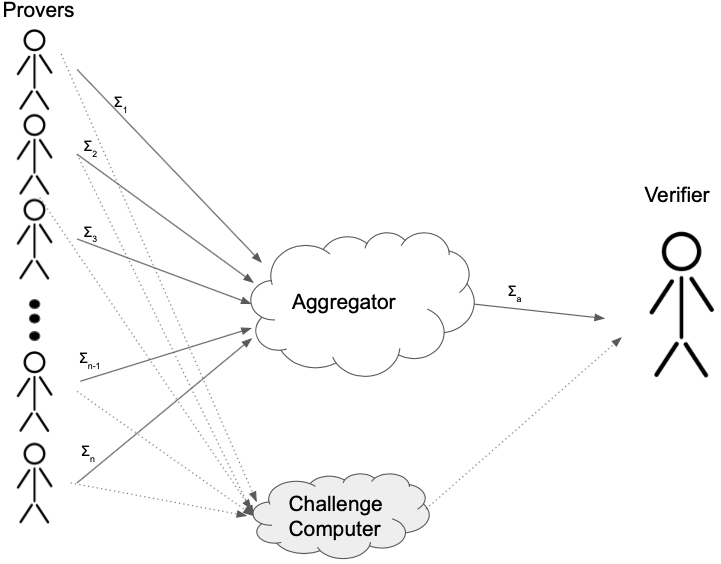
\includegraphics[width=\linewidth]{./figure/oneagg.png}
\caption{Schematic figure of the interaction between Provers, Aggregator and Verifier in aggregated set membership proofs. }
\label{fig:gen_workflow}
\end{figure} 


%TODO fix can this be here?  ONLY range proofs
%A remark is that to aggregate the commitments $C_i, \: i\in\mathcal{S}$ into $C = \prod_{i\in\mathcal{S}} Ci_i$. Then constructing  a range proof that the aggregated commitment $C = g^{\sum_{i=1}^n x_i}$ belongs to the range  $[n\cdot a,n\cdot b]$, does not prove that $x_i \in [a,b]$ for all $i \in\mathcal{N}$. In other word is does not satisfy the verification property in Theorem \ref{thm:VAHSS_RP_CSV}. The value $y=\sum_{i=1}^n x_i$ is publicly known so to construct a zero-knowledge range proof for $y $ provides no new information and given that $y\in [n\cdot a,n\cdot b]$ does not imply $x_i\in [a,b]$ for all $i\in\mathcal{N}$. 


The algorithms of aggregated set membership proofs, presented in Definition \ref{def:GeneralAggregation}, should fulfil the below completeness, soundness and zero-knowledge requirements:
\begin{itemize}
\item \textbf{Completeness} Given a witness $\Sigma_i$ satisfying the instance $x_i\in\Phi$, where $C_i$ is a Pedersen commitment of $x_i$, for all $i\in\mathcal{S}$, it should hold that
\\
 \texttt{Verify}$($\texttt{Aggregate}$(\{$\texttt{Prove}$(pp,i,C_i,\Phi)\}_{i\in\mathcal{S}}) )= 1$. 
\item \textbf{Soundness} If for any $i\in\mathcal{S}$ the  witness $\Sigma_i$ does not satisfy the  instance $x_i\notin\Phi$, then the probability  Prob$[ $\texttt{Verify}$($\texttt{Aggregate}$(\{$\texttt{Prove}$(pp,i,C_i,\Phi)\}_{i\in\mathcal{S}}) ) = 1] < \varepsilon$, for a sufficiently small $\varepsilon$. 
\item  \textbf{Zero-knowledge} 
A proof system is \textit{honest verifier zero-knowledge} if there exists a PPT algorithm \texttt{Simulator} having access to the same input as the algorithms \texttt{Verify} and \texttt{Aggregate} but not the provers input, such that output from the \texttt{Simulator} and \texttt{Prove} is indistinguishable, i.e have the same distribution given that $x\in\Phi$.  
\end{itemize}

These requirements can be seen as a modification of the requirements given in Definition \ref{def:ZKP} to aggregated set membership proof. Note that the zero-knowledge property should hold for the provers, not the aggregation.



%\subsection*{Many aggregation}
%TODO Decise if use

%AGGREGATION
\chapter{Aggregated Signature-Based Set Membership Proofs}
\label{ch:AggSM}
\label{sec:ConstructAggregation}
%TODO fix intro
%In the previous chapter, a definition of aggregated set membership proofs was presented and also the requirements it should fulfil. 
This chapter presents a construction of aggregated set membership proofs derived from the non-interactive signature-based set membership proofs, \cite{RANGE-SET}.   In section \ref{sec:SecurityAggregation} it is proved that the aggregation is sound and in section \ref{sec:CSZKAgg} the completeness, soundness and zero-knowledge requirements, stated in the chapter \ref{ch:generalAgg}, is proved to hold for the aggregated signature-based set membership proofs.
%It is seen that the verification algorithm in Construction \ref{alg:VAHSS-HSS-RP} will be time consuming, since each client is verified individually. Therefore a desired property for the above presented server and clients verifiable AHSS would be to aggregate the range proofs into one, since then the verifier would have to perform one range proof verification instead of one for each client as in Construction \ref{alg:VAHSS-HSS-RP}. This would decrease the runtime for the verification significantly, especially in implementations where many clients participate. 
%TODO require the aggregated to filfil def 4. 
%Aggregating the range proofs would require the proofs to be homomorphic, such that the verification remains valid also for an aggregated proof.

%Argument security of aggregation 
\section{Construction}
%The previous section proposed a design of the algorithm \textbf{Aggregate}, such that the  public signature based set memberships proofs could be partly aggregated. 
Construction \ref{alg:ZKSM-Agg} presents an aggregated signature-based set membership proof, derived from the non-interactive signature-based set membership proofs \cite{RANGE-SET}.

The algorithm \textbf{Aggregate}, in Construction \ref{alg:ZKSM-Agg}, partly aggregates a group of set membership proofs by constructing the aggregated proof,
$\Sigma_a $. The aggregated values $D_a,z_{x_a},z_{R_a}$ in $\Sigma_a$ are computed according to Equation \eqref{eq:aggDn}. 

\begin{equation}
\begin{aligned}
\label{eq:aggDn}
D_a &=\prod_{i\in\mathcal{S}}  D_i ^{\prod_{\substack{j\in\mathcal{S}\\ j\neq i}} c_j }  =  g ^ {\sum_{i\in\mathcal{S}} \Big(\prod_{\substack{j\in\mathcal{S}\\ j\neq i}}   c_j \Big)s_i} h^ {\sum_{i\in\mathcal{S}} \Big( \prod_{\substack{j\in\mathcal{S} \\ j\neq i}}   c_j \Big) m_i}
\\
z_{x_a} &= \sum_{i\in\mathcal{S}} \Big( \prod_{\substack{j\in\mathcal{S}\\ j\neq i}} c_j \Big) z_{x_i} = \sum_{i\in\mathcal{S}} \Big( \prod_{\substack{j\in\mathcal{S}\\ j\neq i}} c_j \Big)s_i - \big( \prod_{j\in\mathcal{S}} c_j \big) \sum_{i\in\mathcal{S}} x_i
\\
z_{R_a} &=  \sum_{i\in\mathcal{S}}  \Big( \prod_{\substack{j\in\mathcal{S}\\ j\neq i}} c_j \Big) z_{R_i} = \sum_{i\in\mathcal{S}} \Big( \prod_{\substack{j\in\mathcal{S}\\ j\neq i}} c_j \Big)m_i - \big( \prod_{j\in\mathcal{S}} c_j \big) \sum_{i\in\mathcal{S}} R_i 
\end{aligned}
\end{equation}

The set $\mathcal{S}$ denotes the index set of the provers and each prover $p_i$ $i\in\mathcal{S}$ publishes a set membership proof $\Sigma_i = (V_i,a_i,D_i,z_{x_i},z_{\tau_i},z_{R_i})$ constructed according to the algorithm \textbf{Prove}. %For all $i\in\mathcal{S}$ the proof $\Sigma_i$ published by the prover $p_i$ is on the form, $\Sigma_i = (V_i,a_i,D_i,z_{x_i},z_{\tau_i},z_{R_i})$.
The challenges, denoted $c_i$ for $i\in\mathcal{S}$, are computed according to the algorithm \textbf{CalculateChallenges}.

The above aggregation has the computational complexity $\mathcal{O}(|\mathcal{S}|^2)$. This is reduced to be linear in $|S|$, by considering the following optimization. Instead of computing the product $\prod_{\substack{j\in\mathcal{S},\: j\neq i}} c_j $ for each $i$, it is sufficient to compute the product $c=\prod_{\substack{j\in\mathcal{S}}} c_j $  once and then the truncated product can be obtained by noting that $ \prod_{\substack{j\in\mathcal{S},j\neq i}} c_j = c/c_i $. Thereby, for each $i\in\mathcal{S}$, it is sufficient to perform one division instead of computing the product $\prod_{\substack{j\in\mathcal{S},\:j\neq i}} c_j $.

Due to the aggregation, the equality $D_a=\prod_{i\in\mathcal{S}}C_i^{\prod_{i\in\mathcal{S}}c_i}h^{z_{R_a}}g^{z_{x_a}}$ is checked once instead of once for each proving party in the protocol. This can bee seen by comparing the algorithm \textbf{Verify} in Construction \ref{alg:ZKSM-Agg} with running the algorithm \textbf{Verify} in Construction \ref{alg:ZKSM} once for each prover. 

\begin{algorithm}[]
\caption{\textbf{: Aggregation of non interactive set membership proof}}
\textbf{Goal:}  Given the Pedersen commitments $C_i=g^{x_i} h^{R_i}$, for $i\in\mathcal{S}$. The construction  proves that all secrets $x_i$ belong to the set $\Phi$, without revealing anything else about the secrets.
\vspace{3pt}\hrule\vspace{2pt}
\begin{itemize}
  \item\text{\textbf{SetUp} $(1^\lambda,\Phi)\xrightarrow[]{}(sk,pp)$}\\
 Let g be a generator of the group $\mathds{G}$ and $h$ an element in the group such that $log_g(h)$ is unknown.  
Pick uniformly at random $\chi\in_R\mathds{F}$ and put $sk=\chi$. Define $y=g^\chi$ and $A_i=g^{\frac{1}{\chi+i}} \:\forall i\in\Phi$, output $pp=(g,h,y,\{A_i\}_{i\in\Phi})$.

\item\text{\textbf{Prove} $(pp,i,C_i,x_i,\Phi)\xrightarrow[]{}\Sigma_i$}\\
Pick uniformly at random $\tau_i\in_R\mathds{F}$, choose from the set $\{A_i\}$ the element $A_{x_i}$ and calculate $V_i=A_{x_i}^{\tau_i}$. Pick uniformly at random three values $s_i,t_i,m_i\in_R\mathds{F}$. Put $a_i=e(V_i,g)^{-s_i}e(g,g)^{t_i}$,  $D=g^{s_i}h^{m_i}$, $c=\text{Hash}(C_i,V_i,a_i,D_i)$ and compute $z_{x_i} = s_i-x_i c_i$, $z_{R_i} = m_i-R_ic_i$ and $z_{\tau_i}= t_i-\tau_i c_i$.  Finally construct and publish the proof $\Sigma_i = (V_i,a_i,D_i,z_{x_i},z_{\tau_i},z_{R_i})$.

\item \text{\textbf{Aggregate} $( pp,\{ \Sigma_i\}_{i\in\mathcal{S}} ) \xrightarrow[]{} \Sigma_a$} \\
Given a set of proofs  $\{\Sigma_i\}_{i\in\mathcal{S}}$. Aggregate the values $( \{D_i \}_{i\in\mathcal{S} }, \{ z_{x_i}\}_{i\in\mathcal{S} }, \{ z_{r_i}\}_{i\in\mathcal{S}  }) \mapsto$ $ D_a,z_{x_a},z_{R_a}$ according to equation \eqref{eq:aggDn}. Construct and publish the aggregated proof $\Sigma_a = (\{V_i\}_{i\in\mathcal{S} },\{a_i\}_{i\in\mathcal{S} },D_a,\{z_{x_i}\}_{i\in\mathcal{S} }, z_{x_a}, \{z_{\tau_i}\}_{i\in\mathcal{S} },z_{R_a})$.

\item \text{ \textbf{CalculateChallenges} $(\{C_i\}_{i\in\mathcal{S}},\{\Sigma_i\}_{i\in\mathcal{S}} ) \xrightarrow[]{} \{c_i\}_{i\in\mathcal{S}}$ }\\
For all $i\in\mathcal{S}$ parse the proof $\Sigma_i$, then compute the challenge $c_i = Hash(C_i,V_i,a_i,D_i)$. Finally output the set of all challenges $\{c_i\}_{i\in\mathcal{S}}$. 

\item\text{\textbf{Verify} $(pp,\Sigma_a,\{C_i\}_{i\in\mathcal{S}},\{c_i\}_{i\in\mathcal{S}}) \xrightarrow[]{} \{0,1\}$} \\
Compute the product of the challenges $c=\prod_{i\in\mathcal{S}} c_i$. Check if $D_a\overset{?}{=} \big( \prod_{i\in\mathcal{S}}C_i\big)^ch^{z_{Ra}}g^{z_{xa}}\wedge a_i \overset{?}{=} e(V_i,y)^c_i e(V_i,g)^{-z_{x_i}}e(g,g)^{z_{\tau_i}}$ for all $i\in\mathcal{S}$. If the equalities hold return $1$ otherwise return $0$.
\end{itemize}
\label{alg:ZKSM-Agg}
\end{algorithm} 


In Construction \ref{alg:ZKSM-Agg} the algorithm \textbf{Prove} is run by all provers, the algorithm \textbf{Aggregate} is run by the aggregating party and the algorithm \textbf{Verify} is performed by the verifier. The algorithm \textbf{SetUp} is assumed to be performed in advance by a trusted party.

In the aggregated signature-based set membership proof the challenges are given as input to the verification algorithm, unlike Construction \ref{alg:ZKSM} where they are computed in the verification algorithm. This raises the question, which party should be responsible for computing the challenges?  It is not desired that the party performing the aggregation computes the challenges since it creates opportunities for cheating.  For the same reason, the proving parties should not compute the challenges. The challenges are constructed according to the Fiat-Shamir heuristic. Two important characteristics of the Fiat-Shamir heuristic are that: the prover does not know the challenge when constructing the proof and that the verifier re-computes the challenge, to check that it is correctly computed.  If the challenges are computed by the aggregating party they are known when constructing the aggregated proof and if they are computed by the provers they are never checked. Thereby, the algorithm \textbf{CalculateChallenges} in Construction \ref{alg:ZKSM-Agg} is assumed to be performed by an honest party independent of both the proving parties and the aggregating party. 

Another alternative is to provide the entire proofs $\{\Sigma_i\}_{i\in\mathcal{S}}$ as input to the verification algorithm, enabling the verifier to compute the challenges. This would consequently increase the computations required by the verifier. For the rest of this paper, if nothing else is mentioned, it is assumed that the algorithm \textbf{CalculateChallenges} is performed according to Construction \ref{alg:ZKSM-Agg} by a trusted party. 

%Comparing the algorithm \textbf{VerifyAggregatedProof} with performing the algorithm \textbf{Verify} in set membership construction once for each clients, it is seen that the first equality check $D \overset{?}{=}( \prod_{i=1}^n C_i )^{c}h^{z_R}g^{z_x}$ is done once instead of once for $|\mathcal{S}|$ times. Construction \ref{alg:ZKSM-Agg} presents all algorithms ,  \textbf{Prove}, \textbf{Aggregate}, \textbf{CalulateChallenges} and \textbf{VerifyAggregatedProof}, needed to build the aggregated set membership proof. 



% , that verifier all individual set membership proof by performing only one verification, resulted in a that a method for aggregating parts of the set membership proof. This method is compiled in Construction \ref{alg:ZKSM-Agg}, where the set membership proof originally presented in \cite{Efficient_proof_interval} is modified to reduce the computational complexity in applications where multiple  proofs are verified simultaneously.

%This leads to that a verification algorithm for verifying the aggregated version of set membership proofs $RP_i$ for $i\in\mathcal{S}$ to be as the algorithm \textbf{VerifyAggregatedProof} in Construction \ref{alg:ZKSM-Agg}.  %TODO 
%\begin{itemize}
%\item\text{\textbf{VerifyAggregatedProof} $(g,h,\{C_i\}_{i\in\mathcal{S}},\{c_i\}_{i\in\mathcal{S}} ,\texit{proof}_{SM,a}) \xrightarrow[]{} \{0,1\}$} \\
%Compute the product of the challenges $c=\prod_{i\in\mathcal{S}} c_i$. Check if $D_a\overset{?}{=} \big( \prod_{i\in\mathcal{S}}C_i\big)^ch^{z_R_a}g^{z_x_a}\wedge a_i \overset{?}{=} e(V_i,y)^c_i e(V_i,g)^{-z_{x_i}}e(g,g)^{z_{\tau_i}}$ for all $i\in\mathcal{S}$. If the equalities holds the provers has convinced the verifier that $x_i\in\Phi$ for all $x_i$ such that $i\in\mathcal{S}$ return $1$ otherwise return $0$.
%\end{itemize}
 
 
\subsection*{Multiple aggregating parties}
To reduce the computational load of the aggregating party it is possible to split the aggregation between multiple parties. %The computational complexity for the algorithm \textbf{Aggregate} is linear in the number of proofs that are aggregated. 

Let the set $\mathcal{K}$ represent the set of parties performing the aggregation, and the set $\mathcal{S}_k$ represent the assigned set of set membership proofs to the $k^{th}$ aggregating party. The sets $\mathcal{S}_k$ for $k\in\mathcal{K}$ are such that $\bigcup_{k\in\mathcal{K}}\mathcal{S}_k = \mathcal{S}$ and $\mathcal{S}_i\bigcap \mathcal{S}_j= \emptyset$ for all $i,j\in\mathcal{K}$ such that $i\neq j$. 

An aggregated signature-based set membership proof, where the aggregation is split between several parties, is presented in appendix \ref{app:manyAggregatingParties} in Construction \ref{alg:ZKSM-Agg-Many}. The adjustments made compared to Construction \ref{alg:ZKSM-Agg} are: the algorithm \textbf{Aggregate} is performed by each party in the set $\mathcal{K}$ on the input $(pp,\{\Sigma_i\}_{i\in\mathcal{S}_k})$, outputting the aggregated proof $\Sigma_{a_k}$. The algorithm \textbf{Verify} is performed once on the input $(pp,\{\Sigma_{a_k}\}_{k\in\mathcal{K}},\{C_i\}_{i\in\mathcal{S}},\{c_i\}_{i\in\mathcal{S}} )$ and  is modified, compared to Construction \ref{alg:ZKSM-Agg}, such that it verifies multiple aggregated proofs. By letting the set of aggregating parties $\mathcal{K}$ consist of one element $k$, and $\mathcal{S}_k  = \mathcal{S}$ constructions \ref{alg:ZKSM-Agg} and \ref{alg:ZKSM-Agg-Many} are equivalent. 
%TODO elaborate


An illustrative figure of how the aggregation is split between the aggregating parties is seen in Figure \ref{fig:workflow}. Each prover generates a set membership proof, and then sends it to its assigned aggregating party. Then each aggregating party aggregates the received set membership proofs, according to the algorithm \textbf{Aggregate} in Construction \ref{alg:ZKSM-Agg-Many}, and sends the aggregated proof to the verifier. Finally the verifier validates all aggregated proofs.

In Figure \ref{fig:workflow} the computation of the challenges is done by an independent party, which introduces a new party to the scheme. To compute the challenges without introducing a new party the aggregating parties can compute the challenges.  However, as discussed previously the same party that aggregates a set of proofs should not compute the challenges for these proofs. To use the aggregating parties for the computations, assume that they are not collaborating and linked in a closed chain. Then each aggregating party computes the challenges for the set of proofs aggregated by the consecutive party in the chain.  
%As discussed previously it would be possible to have the verifier computing the challenges, by additionally giving the proofs $\{ \Sigma_i\}_{i\in\mathcal{N}}$ as input to the verification algorithm. 


 \begin{figure}
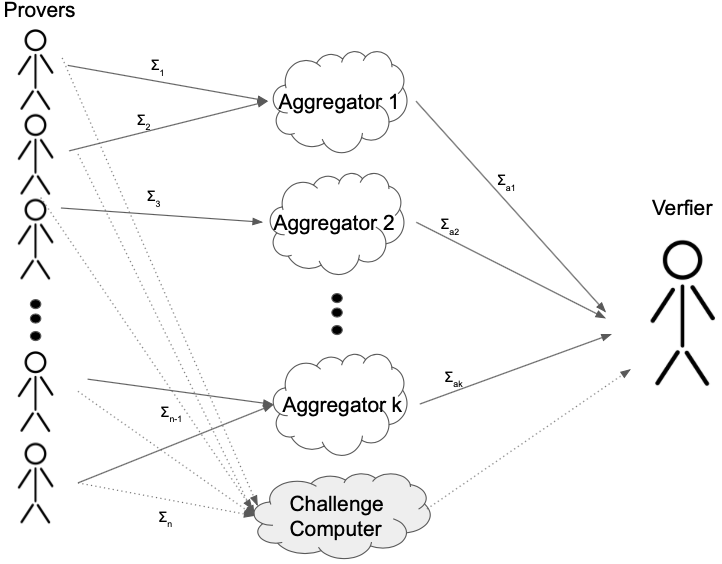
\includegraphics[width=\linewidth]{./figure/splitagg.png}
\caption{Provers outsourcing their set membership proofs to their assigned aggregator that in turn publishes an aggregated set membership proof. }
\label{fig:workflow}
\end{figure} 



%\section{Aggregation of signature based set membership proof}

%In this section the possibility to aggregate the set membership and signature based range proofs  is examined.  The construction of these two are similar and it is sufficient to consider one of them and the conclusion will hold for both constructions. Due to its simpler notation the set membership proof is considered.

%2D example, removed.
\begin{comment}
Again consider the two set membership proofs $\Sigma_1,\Sigma_2$ as defined above, but now restrict the aggregation to only concern half the set membership proof. Namely only terms participating in the the first equality check, $D\overset{?}{=} C^ch^{z_R}g^{z_x}$, in the verification. 

Note that if only a part of the proofs are aggregated it still leads to reduction of computational complexity for the verifier. The goal is now design the aggregation such that the aggregated proof satisfies $D = C^ch^{z_R}g^{z_x}$. 
%Before aggregation calculate the challenges $c_1,c_1$ as $c_i =Hash(D_i,a_i),\:i=1,2$. 
Define the aggregated proof as, $\Sigma_a=(D,z_x,z_R)$, this means the proof does not contain the bilinear maps output $a$ and the group element $V, z_{\tau}$. Further let the the aggregated proof be computed according to, 
\begin{equation}
\label{eq:aggD2}
\begin{aligned}
D &= D_1^{c_2}\cdot D_2^{c_1} = (g^{s_1}h^{m_1}) ^{c_2} \cdot (g^{s_2}h^{m_2}) ^{c_1}  =g^{s_1c_2+s_2c_1}h^{m_1c_2+m_2c_1} \\
z_x &= c_2z_{x_1} +c_1 z_{x_2} = c_2(s_1-x_1c_1)  + c_1(s_2-x_2c_2) = s_1c_2 + s_2c_1 -c_1c_2(x_1+x_2)\\
z_R &= c_2z_{R_1} +c_1 z_{R_2} = c_2(m_1-R_1c_1)  + c_1(m_2-R_2c_2) = m_1c_2 + m_2c_1 -c_1c_2(R_1+R_2)
\end{aligned}
\end{equation}
This construction of the aggregation will result in that the challenges always appears in a product which resolves the problem of them being different. Additionally also define the product of the challenges and commitments as,
\begin{align*}
c &= c_1c_2 \\
C &= C_1C_2 = (g^{x_1}h^{R_1}) (g^{x_2}h^{R_2}) = g^{x_1+x_2}h^{R_1+R_2}.
\end{align*}

%It is assumed that the random values $R_i$ is chosen such that $R_n = \phi(N)\lceil \frac{\sum_{i=1}^{n-1}R_i}{\phi(N)}\rceil- \sum_{i=1}^{n-1}R_i $, which holds for the randomness in a VHASS construction, hence for $i=1,2$ if follows that $R_2 = \phi(N)\lceil \frac{R_1}{\phi(N)}\rceil- R_1$, and thus $h^{c_1c_2(R_1+R_2)} = 1$. 
%This property will not be required for the below calculations, however is does reduce notation and therefore the computations are done under this assumption. 

The aggregated proof $\Sigma_a$, computed according to equation \eqref{eq:aggD2} satisfies the equality $D= C^ch^{z_R}g^{z_x}$, this is seen below,
\begin{align*}
LHS &= D = D_1^{c_2}\cdot D_2^{c_1} =g^{s_1c_2+s_2c_1}h^{m_1c_2+m_2c_1} \\
RHS &= C^ch^{z_R}g^{z_x} = (C_1C_2)^{c_1c_2}h^{c_2z_{R_1}+c_1z_{R_2}}g^{c_2z_{x_1}+c_1z_{x_2}}\\ 
&=(g^{x_1 + x_2})^{c_1c_2} h^{m_1c_2 +m_2c_1} g^{s_1c_2+ s_2c_1- c_1c_2(x_1+x_2)}  \\
&= g^{(x_1+x_2)c_1c_2 - c_1c_2(x_1+x_2) +s_1c_2+s_2c_1} h^{m_1c_2 +m_2c_1} = g^{s_1c_2+s_2c_1} h^{m_1c_2 +m_2c_1} \\
\\ \implies \text{LHS} =\text{RHS}&.
\end{align*}

%This means that this aggregation to construct the proof $RP$ , from the two range proofs $RP_1,RP_2$ as above satisfies the first equality of the verification. 
Aggregation of the two set membership proof defined according to equation  \eqref{eq:aggD2} results in an aggregation that satisfies the  completeness. The next step is to check if this aggregation can be extended to aggregate an arbitrary number of set membership proofs and still satisfy the completeness. 
\end{comment}

%A hint can also be seen in Construction \ref{alg:ZKRP} where the verification of first equity is aggregated while the second is done for each $j\in\mathds{Z}_l$. 




\section{Soundness of Aggregation}
\label{sec:SecurityAggregation}
In this section it is proved that the aggregation must be performed according to the algorithm \textbf{Aggregate} if the aggregated proof $\Sigma_a$ validates true in Construction \ref{alg:ZKSM-Agg}. This is proved under the assumption that: proving parties are not communicating or collaborating between themselves, proving parties are not communicating or collaborating with the aggregating party (or parties), the set membership proof in Construction \ref{alg:ZKSM} is sound and $D_a\neq C^c$.  In this section the product of the Pedersen commitments, $\prod_{i\in\mathcal{S}}C_i$, is denoted $C$ and the product of the challenges, $\prod_{i\in\mathcal{S}} c_i$, is denoted $c$.
%,  where  $C_i$ is a Pedersen commitment of the secret $x_i$ and $c_i$ the challenges used to construct the proofs, $\Sigma_i$, proving that the secret $x_i\in\Phi$, for $i\in\mathcal{S}$. 


If $D_a =  C^c$, it would be possible for an aggregating party to choose the values $D_a,z_{x_a},z_{R_a}$ according to: $D_a =C^c, z_{x_a} = \phi(p), z_{R_a} = \phi(p)$.
%Note that $p$ is the prime underlying the field $\mathds{F}$, $C=\prod_{i\in\mathcal{S}}C_i$ and $c=\prod_{i\in\mathcal{S}}c_i$. 
For the above choice of $D_a,z_{x_a},z_{R_a}$ the equation, $D_a\overset{?}{=} C^c h^{z_{R_a}}g^{z_{x_a}}$ holds trivially true, independent of whether the commitment $C_i$ and the values $z_{x_i}$, thereby $z_{x_a}$, hides the same secret for all $i\in\mathcal{S}$. Therefore it is required that $D_a \neq C^c$.


Under the assumption discussed above, Theorem \ref{thm:aggrgeation} states that the  aggregation must be performed according to the algorithm \textbf{Aggregate} for the algorithm \textbf{Verify} to validate true, in Construction \ref{alg:ZKSM-Agg}. 
\vspace{0.5cm}
\begin{thm}[\textbf{Soundness of aggregation}]
\label{thm:aggrgeation}
Let $\mathcal{A}$ be a PPT adversary. Assume $\mathcal{A}$ has access to the input to the algorithm \textbf{Aggregate} in Construction \ref{alg:ZKSM-Agg} and the Pedersen commitment, $\{C_i\}_{i\in\mathcal{S}}$, but no other information. Assume that the adversary  $\mathcal{A}$ cannot collaborate with the provers, that the provers cannot collaborate with each other and that the set membership proof in Construction \ref{alg:ZKSM} is sound. 

%The provers are not assumed to be honest, but it is assumed that their published proofs are one the form $\Sigma_i = (V_i,a_i,D_i,z_{x_i},z_{\tau_i},z_{R_i})$, where $V_i,D_i\in\mathds{G}$, $a_i\in\mathds{G}_T$ and $z_{x_i},z_{\tau_i},z_{R_i} \in\mathds{F}$, and that the Pedersen commitments $C_i=g^{x_i}h^{R_i}$.


Under these assumptions the adversary $\mathcal{A}$ has a negligible probability of construction $\Sigma_a$ such that: Prob$($\textbf{Verify}$(pp,\Sigma_a,\{C_i\}_{i\in\mathcal{S}},\{c_i\}_{i\in\mathcal{S}}) )=1$, where $D_a\neq C^c$ and  $z_{x_a} \neq \sum_{i\in\mathcal{S}} \Big( \prod_{j\in\mathcal{S}, j\neq i} c_j \big) z_{x_i}$. 


\end{thm}

\begin{proof}
The soundness of signature-based set membership proofs and that the algorithm \textbf{Verify} checks that $a_i\overset{?}{=} e(V_i,y)^{c_i}e(V_i,g)^{-z_{x_i}}e(g,g)^{z_{\tau_i}}$,  for all $i\in\mathcal{S}$, implies that the values $V_i,a_i,z_{x_i},z_{\tau_i}$ of $\Sigma_i$ must be computed according to the algorithm \textbf{Prove} in Construction \ref{alg:ZKSM-Agg}. The values $z_{R_i}$ and $D_i$ are not used directly in the verification, thus the only requirements are that $z_{R_i}\in\mathds{F}$ and $D_i\in\mathds{G}$, for all $i\in\mathcal{S}$.  Assume, without loss of generality that  $D_a=g^\alpha h^\beta$, where $\alpha,\beta\in\mathds{F}$. 

Assume that the adversary $\mathcal{A}$, can construct a valid proof $\Sigma_a$, such that: $D_a\in\mathds{G}$, $z_{x_a},z_{R_a}\in\mathds{F}$ and  $z_{x_a} \neq \sum_{i\in\mathcal{S}} \Big( \prod_{j\in\mathcal{S}, j\neq i} c_j \big) z_{x_i}$. 

%The adversary $\mathcal{A}$ should construct a valid aggregated proof, $\Sigma_a$, i.e choosing the values $D,_az_{x_a},z_{R_a}$. These should be such that $D_a\in\mathds{G}$, $z_x,z_R\in\mathds{F}$ and  $z_{x_a} \neq \sum_{i\in\mathcal{S}} \Big( \prod_{j\in\mathcal{S}, j\neq i} c_j \big) z_{x_i}$. Assume, without loss of generality that  $D_a=g^\alpha h^\beta$, where $\alpha,\beta\in\mathds{F}$. 

For the aggregated proof to be valid it must hold that $D_a= C^ch^{z_{R_a}}g^{z_{x_a}}$ which implies that the values $\alpha,\beta,z_{x_a},z_{R_a}$ must satisfy:
\begin{align*}
g^\alpha h^\beta  = C^cg^{z_{x_a}}h^{z_{R_a}}.
\end{align*}
The values of $C^c $ cannot be modified by the adversary since it is sent directly from the provers to the verifier. The Pedersen commitments are assumed to be on the form $C_i= g^{x_i}h^{R_i}$ for all $i\in\mathcal{S}$ and the challenges are correctly computed and checked by a trusted party.

Consequently, by expanding the right hand side of the equality it follows that,
\begin{align*}
g^\alpha h^\beta =  g^{c \sum_{i\in\mathcal{S}}x_i +z_{x_a} } h^{ c \sum_{i\in\mathcal{S}}R_i +z_{R_a}   }.
\end{align*}

If $\alpha \neq c \sum_{i\in\mathcal{S}} x_i+z_{x_a}$ and $\beta\neq c\sum_{i\in\mathcal{S}}R_i +z_{R_a}$, the above equality contradicts to the binding property of the Pedersen commitments.  %assumption that it is not possible to construct two equal Pedersen Commitments hiding different secrets.
Thereby, the values $\alpha, \beta , z_{x_a}$ and $z_{R_a}$ must satisfy: 
$\alpha =  c \sum_{i\in\mathcal{S}} x_i+z_{x_a}$ 
and 
$\beta =  c \sum_{i\in\mathcal{S}} R_i +z_{R_a}$.  

This can be rewritten as $\alpha-z_{x_a} =  c \sum_{i\in\mathcal{S}} x_i$ mod $\Phi(p)$ and  $\beta-z_{R_a} =  c \sum_{i\in\mathcal{S}} R_i$ mod $\Phi(p)$. The sums $ \sum_{i\in\mathcal{S}} x_i$ and $ \sum_{i\in\mathcal{S}} R_i$ are assumed to be unknown.  

Thereby, under the assumption that $z_{x_a}\neq \sum_{i\in\mathcal{S}} \Big( \prod_{j\in\mathcal{S}, j\neq i} c_j \big) z_{x_i} $ the adversary has a negligible probability of choosing $\alpha,\beta,z_{x_a},z_{R_a}$ such that $D_a= C^ch^{z_{R_a}}g^{z_{x_a}}$. It follows that  $z_{x_a} = \sum_{i\in\mathcal{S}} \Big( \prod_{j\in\mathcal{S}, j\neq i} c_j \big) z_{x_i}$, which contradicts the assumption and proves the theorem. 


\end{proof}
Note that the theorem would still hold even if several untrusted parties aggregated subsets of the proofs and a verifier validated all the aggregated proofs. 

\section{Completeness, Soundness and Zero-Knowledge}
\label{sec:CSZKAgg}
In this section, it is proved that Construction \ref{alg:ZKSM-Agg}  fulfils the completeness, soundness and zero-knowledge requirements stated in chapter \ref{ch:generalAgg}. This is proved under the  assumption that the aggregation is performed according to the algorithm \textbf{Aggregate},  provers cannot communicate or collaborate with each other and that Construction \ref{alg:ZKSM} satisfies the requirement stated in Definition \ref{def:ZKP}.
% The assumption that the aggregation is performed by a trusted party %TODO
 The requirements also hold for Construction \ref{alg:ZKSM-Agg-Many}, considering $|\mathcal{K}|>1$.

\subsubsection*{Completeness}
To prove the completeness of Construction \ref{alg:ZKSM-Agg}, it has to be proved that\\ \textbf{Verify}$ ( $\textbf{Aggregate}$ (\{ $\textbf{Prove}$ (pp,i,C_i,x_i,\Phi)\}_{i\in\mathcal{S}}) )= 1$. To prove this, let $\Sigma_i$ for $i\in\mathcal{S}$ denote proofs constructed by the algorithm \textbf{Prove} and $\Sigma_a $ denote the aggregation of these proofs obtained according to algorithm \textbf{Aggregate}. For all $i\in\mathcal{S}$, let $C_i$ denote the Pedersen commitment of the secrets $x_i$ and $c_i$ denote the challenge used in the proof.

Then by the completeness property of the signature-based set membership proof \cite{RANGE-SET}, it holds that:
\begin{align*}
a_i = e(V_i,y)^{c_i}e(V,g)^{z_{x_i}}e(g,g)^{z_{\tau_i}} \:\: \forall \: i\in\mathcal{S}.
\end{align*}

It remains to argue that $D_a =C^ch^{z_{R_a}}g^{z_{x_a}}$, where $C=\prod_{i\in\mathcal{S}}C_i$ and $c=\prod_{i\in\mathcal{S}}c_i$. By construction it holds that:
\begin{align*}
D_a = &g ^ {\sum_{i\in\mathcal{S}} \Big(\prod_{\substack{j\in\mathcal{S}\\ j\neq i}}   c_j \Big)s_i} h^{\sum_{i\in\mathcal{S}} \Big(\prod_{\substack{j\in\mathcal{S}\\ j\neq i}}    c_j \Big)m_i}  ,
\\
 C^ch^{z_{R_a}}g^{z_{x_a}} =&\:  \Big( \prod_{i\in\mathcal{S}} C_i \Big)^{\prod_{i\in\mathcal{S}} c_i}h^ {\sum_{i\in\mathcal{S}} \Big( \prod_{\substack{j\in\mathcal{S}\\ j\neq i}}   c_j \Big)m_i}
g^{ \sum_{i\in\mathcal{S}} \Big( \prod_{\substack{j\in\mathcal{S}\\ j\neq i}}   c_j \Big)s_i - \big( \prod_{j\in\mathcal{S}} c_j \big) \sum_{i\in\mathcal{S}} x_i}
\\ 
 = &\Big( g^{\sum_{i\in\mathcal{S}} x_i} h^{\sum_{i\in\mathcal{S}} R_i}\Big)^{\prod_{i\in\mathcal{S}} c_i} h^{ \sum_{i\in\mathcal{S}} \Big( \prod_{\substack{j\in\mathcal{S}\\ j\neq i}} c_j \Big)m_i - \big( \prod_{j\in\mathcal{S}} c_j \Big) \sum_{i\in\mathcal{S}} R_i  }
 \\
 &g^{ \sum_{i\in\mathcal{S}} \Big( \prod_{\substack{j\in\mathcal{S}\\ j\neq i}}   c_j \Big)s_i - \big( \prod_{j\in\mathcal{S}} c_j \big) \sum_{i\in\mathcal{S}} x_i} \\
 =  &g^{ \sum_{i\in\mathcal{S}} \Big( \prod_{\substack{j\in\mathcal{S}\\ j\neq i}}  c_j \Big)s_i } h^{\sum_{i\in\mathcal{S}} \Big( \prod_{\substack{j\in\mathcal{S}\\ j\neq i}}   c_j \Big)m_i}  ,
\\
 \implies D_a \:=& \:C^ch^{z_{R_a}}g^{z_{x_a}}
\end{align*}

Combining the above results it has been shown that $D_a  = C^ch^{z_{Ra}}g^{z_{xa}}\wedge a_i = e(V_i,y)^c_i e(V_i,g)^{-z_{x_i}}e(g,g)^{z_{\tau_i}}$ for all $i\in\mathcal{S}$.
Implying that \textbf{Verify}$ ( $\textbf{Aggregate}$ (\{ $\textbf{Prove}$($
$pp,i,C_i,x_i,\Phi)\}_{i\in\mathcal{S}}) )= 1$.
%To aggregate the public signature based set membership proofs possible constructions for the algorithm \textbf{Aggregate} is evaluated. The starting point for designing such a construction is that the aggregation of public signature set membership proofs according to the algorithm \textbf{Aggregate} should result in construction that satisfies the completeness requirement in Definition \ref{def:ZKP_agg}. Remark that it is assumed that the verification of the aggregated proof should be designed in the same way as the algorithm \textbf{Verify} in Construction \ref{alg:ZKSM}. Having found an implementation of the algorithm \textbf{Aggregate} that satisfies the completeness it will then be examined under what assumptions the soundness and zero-knowledge in Definition \ref{def:ZKP_agg} is satisfied. 

%To investigate different designs of the algorithm \textbf{Aggregate} and whether it  provides an aggregated set membership proof that satisfies the completeness the following is considered. 


%Consider $|\mathcal{S}|$ provers and consequently  $|\mathcal{S}|$ set membership proofs denoted $\Sigma_i,\: i\in\mathcal{S}$. The aggregation in equation \eqref{eq:aggD2} extended to aggregate all proof results in the aggregation procedure below,
%\begin{equation}
%\label{eq:aggDn}
%\begin{aligned}
%D &=\prod_{i\in\mathcal{S}}  D_i ^{\prod_{\substack{j\in\mathcal{S}\\ j\neq i}} c_j }  =  \prod_{i\in\mathcal{S}}  (g^{s_i}h^{m_i}) ^{\prod_{\substack{j\in\mathcal{S}\\ j\neq i}}  c_j } = g ^ {\sum_{i\in\mathcal{S}} \Big(\prod_{\substack{j\in\mathcal{S}\\ j\neq i}}   c_j \Big)s_i} h^ {\sum_{i\in\mathcal{S}} \Big(\prod_{\substack{j\in\mathcal{S}\\ j\neq i}}   c_j \Big)m_i} \\
%z_x &= \sum_{i\in\mathcal{S}} \Big( \prod_{\substack{j\in\mathcal{S}\\ j\neq i}} c_j \Big) z_{x_i} = \sum_{i\in\mathcal{S}} \Big( \prod_{\substack{j\in\mathcal{S}\\ j\neq i}} c_j \Big)s_i - \big( \prod_{j\in\mathcal{S}} c_j \big) \sum_{i\in\mathcal{S}} x_i\\
%z_R &=  \sum_{i\in\mathcal{S}}  \Big( \prod_{\substack{j\in\mathcal{S}\\ j\neq i}} c_j \Big) z_{R_i} = \sum_{i\in\mathcal{S}} \Big( \prod_{\substack{j\in\mathcal{S}\\ j\neq i}} c_j \Big)m_i - \big( \prod_{j\in\mathcal{S}} c_j \big) \sum_{i\in\mathcal{S}} R_i 
%\end{aligned}
%\end{equation}
%Let $C=\prod_{i\in\mathcal{S}} C_i$ be the product of all Pedersen commitments and $c= \prod_{i\in\mathcal{S}} c_i$ the product of the challenges.  The partly aggregated set membership proof $\Sigma_a = (D,z_x,z_r)$ computed according to equation \ref{eq:aggDn} satisfies $D= C^ch^{z_R}g^{z_x}$, 
%\begin{align*}
%LHS =& D = g ^ {\sum_{i\in\mathcal{S}} \Big(\prod_{\substack{j\in\mathcal{S}\\ j\neq i}}   c_j \Big)s_i} h^ {\sum_{i\in\mathcal{S}} \Big(\prod_{\substack{j\in\mathcal{S}\\ j\neq i}}    c_j \Big)m_i}  
%\\
%RHS =& C^ch^{z_R}g^{z_x} =  \Big( \prod_{i\in\mathcal{S}} C_i \Big)^{\prod_{i\in\mathcal{S}} c_i}h^ {\sum_{i\in\mathcal{S}} \Big( \prod_{\substack{j\in\mathcal{S}\\ j\neq i}}   c_j \Big)m_i}
%\\
%&g^{ \sum_{i\in\mathcal{S}} \Big( \prod_{\substack{j\in\mathcal{S}\\ j\neq i}}   c_j \Big)s_i - \big( \prod_{j\in\mathcal{S}} c_j \big) \sum_{i\in\mathcal{S}} x_i}
%\\ 
% =& \Big( g^{\sum_{i\in\mathcal{S}} x_i} h^{\sum_{i\in\mathcal{S}} R_i}\Big)^{\prod_{i\in\mathcal{S}} c_i} h^{ \sum_{i\in\mathcal{S}} \Big( \prod_{\substack{j\in\mathcal{S}\\ j\neq i}} c_j \Big)m_i - \big( \prod_{j\in\mathcal{S}} c_j \Big) \sum_{i\in\mathcal{S}} R_i  }
% \\
% &g^{ \sum_{i\in\mathcal{S}} \Big( \prod_{\substack{j\in\mathcal{S}\\ j\neq i}}   c_j \Big)s_i - \big( \prod_{j\in\mathcal{S}} c_j \big) \sum_{i\in\mathcal{S}} x_i}=  g^{ \sum_{i\in\mathcal{S}} \Big( \prod_{\substack{j\in\mathcal{S}\\ j\neq i}}  c_j \Big)s_i } h^{\sum_{i\in\mathcal{S}} \Big( \prod_{\substack{j\in\mathcal{S}\\ j\neq i}}   c_j \Big)m_i}  
%\\
% \implies \text{LHS} =& \text{ RHS}.
%\end{align*}

%TODO who aggregates, how do you ensure the aggregation is correct, challanges not possible for the verifier to compute since do not know the D_i and a_i and so on. Could you have a homoporphic hashfunction so this is not an issue? Or not since Di^{\prod{c_j}}... 

%TODO cleatify who does who and how the new verification would look. Could servers do it? Or would they then be able to indluence to their favour ? 

%TODO 1) assume aggregation correct, can client cheat? 
% 2) can aggregation be done not correct?
%Above it has been seen that arbitrary many set memberships proofs can be aggregated according to equation \eqref{eq:aggDn} such that $D=C^ch^{z_R}g^{z_x}$,  holds after the aggregation. This results in a technique to aggregate  set membership proofs such that when verifying the signature based set membership proofs the first equality, $D=C^cg^{z_x}h^{z_R}$, only need to be verified once instead of once once for each proof.

%Next examine if the entire construction of public signature based set membership proofs can be aggregated. This implies that in addition to the above aggregation the second equality should also be satisfied after aggregating. This leads to that aggregated proof should be equal to  $\Sigma_a = (a,V,D,z_x,z_\tau,z_R)$ where the values $a,V,z_x,z_\tau$ satisfies the equation $a = e(V,y)^c e(V,g)^{-z_x}e(g,g)^{z_\tau}$. 


%Completeness follows from the argument given above, where it has been seen that $D\overset{?}{=}C^ch^{z_R}g^{z_x}$ given all parties where honest, and the completeness of the public signature based set membership proof. Thereby Construction \ref{alg:ZKSM-Agg} satisfies the completeness in Definition \ref{def:ZKP_agg}. 

\subsubsection*{Zero-Knowledge}
The zero-knowledge property of Construction \ref{alg:ZKSM-Agg} follows from the zero-knowledge property of Construction \ref{alg:ZKSM} and by realising that the algorithm \textbf{Aggregate} does not reveal any information about the secrets $x_i$ for any $i\in\mathcal{S}$. The latter follows from multiplying and adding elements perfectly hiding the secret $x_i$, with other elements independent of the secret $x_i$ does not reveal any information about the secret. 

\subsubsection*{Soundness}
The aggregated set membership proof in Construction \ref{alg:ZKSM-Agg} satisfies the soundness property stated in chapter \ref{ch:generalAgg} under the assumptions that the aggregation is performed according to the algorithm \textbf{Aggregate} in Construction \ref{alg:ZKSM-Agg},  that provers cannot communicate or collaborate and that the set membership proof in Construction \ref{alg:ZKSM} satisfies the soundness in Definition \ref{def:ZKP}. To prove this it has to be shown that if for any $i\in\mathcal{S}$ the secret $x_i\notin\Phi$ then it holds that \\ Prob$[ $\textbf{Verify}$($\textbf{Aggregate}$(\{$\textbf{Prove}$(pp,i,C_i,x_i,\Phi)\}_{i\in\mathcal{S}}) ) = 1] < \varepsilon$, for some negligible $\varepsilon$.


Let $T$ denote the index-set of the malicious provers. Assume that all honest provers $p_i$, such that $i\in\mathcal{S}\backslash T$, computes their set membership proofs, $\Sigma_i$, according to \textbf{Prove}.


%TODO fixa mening
If the algorithm \textbf{Verify} validates true then $a_i=e(V_i,y)^{c_i}e(V,g)^{z_{x_i}}e(g,g)^{z_{\tau_i}}$ for all $i\in\mathcal{S}$. Thereby the soundness assumption of the set membership proofs in Construction \ref{alg:ZKSM} implies that the values $a_i,V_i,z_{x_i},z_{\tau_i}$ must be computed according to the algorithm \textbf{Prove} in Construction $\ref{alg:ZKSM-Agg}$.
%Thereby a malicious client has to commit values of $D_i,z_{R_i}$ such that after aggregation the the algorithm \textbf{VerifyAggregted} validates true while the Pedersen commitment $C_i$ and value $z_{x_i}$ are such that $x_i\neq\tilde{x_i}$, such that $x_i\in\Phi$ and $\tilde{x}_i \notin\Phi$.
Implying that the malicious provers, $p_i$ for $i\in T$, must construct their set membership proofs, $\Sigma_i$, and Pedersen commitments, $C_i$, such that the following is fulfilled:
\begin{align*}
V_i &= A_{x_i}^{\tau_i}, 				  		&a_i& = e(V_i,g)^{-s_i}e(g,g)^{t_i}, 		\\
D_i &= g^{\tilde{s}_i}h^{\tilde{m}_i},		&z_{x_i}& = s_i-x_ic_i,							\\
z_{\tau_i} &= t_i- \tau_i c_i, 					&z_{R_i}&\in \mathds{F},					\\
C_i &= g^{\tilde{x}_i}h^{\tilde{R}_i},
\end{align*}
where $\tilde{x}_i\neq x_i$ and $x_i\in\Phi$. It is not required that $\tilde{s}_i =s_i$, $\tilde{m}_i =m_i$, $\tilde{R}_i =R_i$ are equalities nor inequalities.

For the algorithm \textbf{Verify} to validate true it has to hold that $D_a=C^ch^{z_{R_a}}g^{z_{x_a}}$, where $D_a,z_{R_a},z_{x_a}$ is the aggregation of $\Sigma_i$ for all $i\in\mathcal{S}$  according to equation \eqref{eq:aggDn}. By expanding the equality it follows that:
\begin{align*}
D_a =& g ^ {\sum_{i\in T } \Big(\prod_{\substack{j\in\mathcal{S}\\ j\neq i}}   c_j \Big)\tilde{s}_i + \sum_{i\in\mathcal{S}\backslash T } \Big(\prod_{\substack{j\in\mathcal{S}\\ j\neq i}}   c_j \Big)s_i} h^ {\sum_{i\in T } \Big(\prod_{\substack{j\in\mathcal{S}\\ j\neq i}}    c_j \Big)\tilde{m}_i+ \sum_{i\in\mathcal{S}\backslash T} \Big(\prod_{\substack{j\in\mathcal{S}\\ j\neq i}}    c_j \Big)m_i } 
 \\
 C^ch^{z_{R_a}}g^{z_{x_a}} =&   \Big( g^{\sum_{i\in T} \tilde{x}_i + \sum_{i\in \mathcal{S}\backslash T} x_i} h^{\sum_{i\in T} \tilde{R}_i + \sum_{i\in \mathcal{S}\backslash T} R_i}  \Big) ^{\prod_{j\in\mathcal{S}} c_j}  h^{ \sum_{i\in T } \Big( \prod_{\substack{j\in\mathcal{S}\\ j\neq i}} c_j \Big) z_{R_i}}
 \\
& h^{\sum_{i\in\mathcal{S}\backslash T } \Big( \prod_{\substack{j\in\mathcal{S}\\ j\neq i}}   c_j \Big) m_i - \sum_{i\in\mathcal{S} \backslash T} \big( \sum_{i\in\mathcal{S}} c_j\big)R_i}  
g^{ \sum_{i\in\mathcal{S}} \Big( \prod_{\substack{j\in\mathcal{S}\\ j\neq i}}   c_j \Big)s_i - \big( \prod_{j\in\mathcal{S}} c_j \Big) \sum_{i\in\mathcal{S}} x_i}
\\ 
 &=  g ^{\prod_{j\in\mathcal{S}} c_j \big(\sum_{i\in T} \tilde{x}_i + \sum_{i\in T} x_i\big) +  \sum_{i\in T} \big( \prod_{\substack{j\in\mathcal{S}\\ j\neq i}} c_j\big) s_i     } h^{ \big(\prod_{j\in\mathcal{S}} c_j\big)\sum_{i\in T} \tilde{R}_i  + \sum_{i\in T } \Big( \prod_{\substack{j\in\mathcal{S}\\ j\neq i}} c_j \Big) z_{R_i} }
\\
& 
g ^ {\sum_{i\in\mathcal{S}\backslash T } \Big(\prod_{\substack{j\in\mathcal{S}\\ j\neq i}}   c_j \Big)s_i} h^ { \sum_{i\in\mathcal{S}\backslash T} \Big(\prod_{\substack{j\in\mathcal{S}\\ j\neq i}}    c_j  \Big) m_i} .
\end{align*}

Both above equations can be interpreted as Pedersen commitments.  It is assumed, under the discrete logarithm assumption, that two Pedersen commitments cannot be equal unless their arguments are equal. This implies that the exponents of $g$ and $h$ are equal for the two above equations. Consider the exponent of $g$ this leads to:
\begin{align}
\label{eq:cheatingCient}
\sum_{i\in T} \big(\prod_{\substack{j\in\mathcal{S}\\ j\neq i}} c_j \big) \tilde{s}_j =& \prod_{j\in\mathcal{S}} c_j \big(\sum_{i\in T} \tilde{x}_i + \sum_{i\in T} x_i\big) + \sum_{i\in T} \big( \prod_{\substack{j\in\mathcal{S}\\ j\neq i}} c_j\big) s_i  . 
\end{align}

It remains to argue that the equality in equation \eqref{eq:cheatingCient} cannot hold unless $\tilde{x}_i= x_i$ for all $i\in\mathcal{S}$.

First consider the case when the set $T$ only consists of one element, implying that there is only one malicious prover. Without loss of generality assume that this is the k$^{th}$ prover, $p_k$. Under this assumption equation \eqref{eq:cheatingCient} can be rewritten as, 
\begin{align*}
\big(\prod_{\substack{j\in\mathcal{S}\\ j\neq k}} c_j \big)  \tilde{s}_k  =& \big ( \prod_{\substack{j\in\mathcal{S}\\ j\neq k}} c_j \big)c_k \big( \tilde{x}_k + x_k\big) +\big( \prod_{\substack{j\in\mathcal{S}\\ j\neq k}} c_j\big) s_k  \implies   \tilde{s}_k  = c_k \big( \tilde{x}_k + x_k\big) + s_k
\end{align*}
If it would be possible to choose $\tilde{s}_k = c_k \big( \tilde{x}_k + x_k\big) + s_k $, it would contradict the soundness assumption of Construction \ref{alg:ZKSM}. Thereby if $|T|=1$, it must hold that $\tilde{x}_k=x_k$.

%TODO define random more clear
Assume $|T|>1$ and $k\in T$ such that  $p_k$ is a malicious prover. Under the assumption that the provers cannot communicate or collaborate, the proofs $\{\Sigma_i\}_{\substack{i\in\mathcal{S}, i\neq k}}$, can be considered random values for the  prover $p_k$. Equation \eqref{eq:cheatingCient} can be rewritten as:
\begin{align*}
\big(\prod_{\substack{j\in\mathcal{S}\\ j\neq i}} c_j \big) \tilde{s}_k +  \overbrace{\sum_{\substack{i\in T \\ i\neq k}} \big(\prod_{\substack{j\in\mathcal{S}\\ j\neq i}} c_j \big) \tilde{s}_j}^{\text{Random }}  &=
  \big ( \prod_{\substack{j\in\mathcal{S}\\ j\neq k}} c_j \big)c_k \big( \tilde{x}_k + x_k\big) +\big( \prod_{\substack{j\in\mathcal{S}\\ j\neq k}} c_j\big) s_k 
  \\ 
   &+ \overbrace{\prod_{j\in\mathcal{S}} c_j \big(\sum_{\substack{i\in T \\ i\neq k}} \tilde{x}_i + \sum_{\substack{i\in T \\ i\neq k}} x_i\big)}^{\text{Random}} \\
   & + \overbrace{\sum_{\substack{i\in T \\ i\neq k}} \big( \prod_{\substack{j\in\mathcal{S}\\ j\neq i}} c_j\big) s_i  }^{\text{Random}}
\end{align*}
If $\tilde{x}_k \neq x_k$, this would imply that it is possible to cheat in Construction \ref{alg:ZKSM} by adding random values to $D_i$ and $z_{x_i}$. This is a contradiction to the soundness assumption of the set membership proof in Construction \ref{alg:ZKSM}. This implies that $\tilde{x}_k=x_k$. 

Thereby, it is proved that if for any $i\in\mathcal{S}$ the secret  $x_i\notin \Phi$, it holds that Prob$[ $\textbf{Verify}$($\textbf{Aggregate}$(\{$\textbf{Prove}$(pp,i,C_i,x_i,\Phi)\}_{i\in\mathcal{S}}) ) = 1] < \varepsilon$, for a negligible $\varepsilon$.

\vspace{10pt}
\begin{thm}[\textbf{Completeness, Zero-Knowledge and Soundness}]
Assume that the aggregated proof $\Sigma_a$ is computed according to algorithm \textbf{Aggregate} in Construction \ref{alg:ZKSM-Agg},  that the parties constructing the proofs, $\{\Sigma_i\}_{i\in\mathcal{S}}$, cannot communicate and that the set membership proof in Construction \ref{alg:ZKSM} satisfies the requirements stated  in Definition \ref{def:ZKP}.
Then the  aggregated signature-based set membership proof in Construction \ref{alg:ZKSM-Agg} satisfies the completeness, zero-knowledge and soundness requirements for aggregated set membership proofs, stated in chapter \ref{ch:generalAgg}.
\end{thm}
\begin{proof}
The proof follows from the arguments given above. 
\end{proof}
%It has been proved that the aggregated set membership proof, presented in Construction \ref{alg:ZKSM-Agg}, fulfils the soundness in Definition \ref{def:ZKP_agg} under the assumptions that the aggregation is performed according to equation \eqref{eq:aggDn} by a trusted party, that provers cannot communicate and that the set membership proof in Construction \ref{alg:ZKSM} is sound. 
%\end{proof}
% c be partially aggregated by servers, not compleatly by aggregator of RP -> alll c_i used most be correct?

%More precisely it has to hold that a secret not in $\Phi$ satisfies the verification with a negligible property and additionally that the secret hidden in the commitments $C_i$ is the same as the secrets in $z_{x_i}$. 


%Neither the  second equality test including  bilinear mapping holds after aggregation, this equality will not hold even if the challenges are equal, i.e $c_1=c_2$ unlike the first.  This concludes that the neither set membership nor signature based range proof can be straight forward aggregated without modifications.  Challange in included on both sides, is this an issue? But not yout own challange on LHS?

%TODO read above and includeref to contsuction 8. 



%The arguments given for the assumptions of the aggregating party and arguments for the aggregated proof satisfying the completeness, soundness and zero-knowledge  does not act as formal proofs, it should rather be seen an as motivations. therefore all potential attacks on aggregated set membership proof can not be deducted and before using it in practise further security checks need to be performed. 




%\subsection*{Aggregating Bulletproofs}
 %The original paper about Bulletproofs \cite{bulletProofs_theory} presents a method to aggregate Bulletproofs such that $n$ parties each having a Pedersen commitment $C_i,\: i=1,...,n$ can generate a single Bulletproof verifying that each commitment hides a secret in an allowed range. The presented approach only works if all parties uses the same challenge $c$ in the proof construction, this is achieved by introducing a dealer. During the constructions of the proofs when computing the challenges each client sends their proof of to this point to the dealer who aggregates the proofs and computes the challenges based on the aggregated proofs. For example, assume $n$ clients and denote their respective proofs with a subscript $i$, then to compute the challenges $y_i$ in construction \ref{alg:bullet} instead of each client computing $y_i = Hash(A_i,S_i)$, each client sends $A_i,S_i$ to the dealer who adds then homomorphically $A = \prod_{i=1}^n A_i, S = \prod_{i=1}^n S_i$ and the send back the challenge $y =Hash(A,S)$ to be use by all clients. This procedure is repeated for each challenge. 
 
 %It is noted that although the Fiat-Shamir heuristic is used to generate the challenges the construction is interactive since communication between the dealer and the clients is required during the construction of the aggregated range proof. If this procedure was ignored and each client instead computed their own challenges via Fiat-Shamir heuristic and the proof where aggregated after they were fully constructed,  then the challenges would differ between parties and the verification fail. 

%Concluding, it has been seen that the  Bulletproof can be aggregated with the cost on an  interactive construction, however this is not a desirable property for the the server and client verifiable AHSS. Investigation about whether this construction can be modified to be completely non-interactive has not been done and remains an open question.  

%This concludes that neither of the considered range proofs has be sucessfully fully aggregated aggregated  such that the verifier can perform one single verification instead of one for each client, at least not without some cost. Remark that this conclusion is not final and their may very well exist small or large modifications of the range proof that will allow them to be aggregated and still remaining non-interactive. The investigation of such modification is outside the scope of this paper but the reader is endorsed to explore this possibility. 


% METHODS
%\chapter{Methods}
\label{ch:Methods}

The purpose of this chapter is to based on the theory given in the chapter present an extended VAHSS construction that ensures honest clients by verifying that their inputs is from an allowed range or set. This will be done by first evaluating the performance of the range proofs discussed above to get an understanding of their advantages and disadvantages plus some indications to their runtime. Then in section \ref{sec:combination} details on how to create a construction of a VAHSS that ensures honest clients is presented and its correctness is proven. In section \ref{sec:implement} details about how to implement this construction is discussed. 

\section{Comparison of range proofs}
In this section the different constructions for verifying clients honesty presented in section \ref{sec:RF_theory} will be analysed and compared in order to evaluate  their suitability to combine with the VAHSS scheme described in Construction \ref{alg:VAHSS-HSS} to verify clients honesty. First a theoretical analysis of each range proofs will given and then a prototype analysis where the range proofs are compares.  

The aspects that will be considered in the evaluation of the range proofs and their compatibility with the VAHSS construction is presented is the below list;
\begin{itemize}
    \item Proof size (communication complexity)
    \item Computation complexity  (for setup, prover verifier)
    \item Flexibility of range
\end{itemize}

Remark that all of the range proof considered aim to prove that the secret in a Pedersen commitment is in an allowed range. Thus to combine any of the range proofs with the VAHSS construction, the clients needs to published Pedersen commitment of their secret $x_i$. This is investigated further in section \ref{sec:combination} and it will be shown that the adaptation of the VAHSS construction to include a range proof is the same independent of the range proof used, hence the adaptability to VAHSS in not relevant in the evaluation in this section.

The considerable difference between the bulletproof and the signature based range proofs makes the comparison between them not straightforward.  Signature based range proofs requires bilinear mappings unlike bulletproofs, bilinear mappings are relative expensive operation compared to for example group exponentials which are dominating  the computational complexity for bulletproofs. Therefore it is not straightforward to compare them in aspects of number of operations performed and an explicit comparison will only be made with respect to runtime. But first the theoretical performance of the range proofs will be discussed individually.

\subsection{Theoretical analysis: Signature-based set membership and range proof}

First lets discuss the communication complexity and proof size starting with the signature based set membership . This construction allows for a $\mathcal{O}(1)$- size proof that a committed value belongs to a given set $\Phi$. In order to construct such a proof $n=|\Phi|$ digital signatures needs to be known by both prover and verifier, one signature for each elements in $\Phi$. This signatures are usually shared by the verifier in the Setup phase. Sharing the digital signatures of the elements in the set $\Phi$ becomes intractable when the set is large.  A large set in this context would be a set consisting of a few hundred elements since the verifier has to publish $n$ digital signatures in the SetUp phase. 

The signature based range proof reduces this to only needing to publish $u$ digital signatures to prove a commitment is in the range $[0,u^l]$ in the SetUp phase. In the algorithm \textbf{Prove} in Construction \ref{alg:ZKRP} the prover sends $l+1$ elements from the group $\mathds{G}_1$, $l$ elements from the group $\mathds{G}_T$ and $2l+1$ field elements. Comparing to the algorithm \textbf{Prove} in Construction \ref{alg:ZKSM} where the prover sends two elements from the group $\mathds{G}_1$, one elements from the group $\mathds{G}_T$ and three field elements. For the ZKRP the communication complexity depends on the choice of $u,l$. Asymptotic analysis gives a communication complexity $\mathcal{O}(\frac{k}{log\:k-log\:log\:k})$, where $l=\frac{k}{log\:u}$ and $u$ put to $u=\frac{k}{log\: k}$ Here $k$ satisfies $u^l \geq 2^{k-1}$.

For ZKSM the communicational complexity for the proof is lower then for the ZKRP, given $l>1$. In some practical applications the digital signatures shared in the setup phase can be assumed to be pre shared, for example in applications where $\Phi$ is used many times. This leads that ZKSM is to prefer over ZKRP in such applications or when $\Phi$ is a relative small. 

Next consider the computational complexity for algorithms \textbf{Prove} and \textbf{Verify} in the ZKSM and ZKRP. constructions  In the set membership construction both the prover and verifier has to perform one bilinear paring and two exponentials over the group $\mathds{G}$. While in the range proof construction the prover need to perform $l$ bilinear mappings and $5l$ exponentials to prove a secret is in the range $[0,u^l)$ and additionally $3l$ exponentials for arbitrary ranges $[a,b]$. The verifier need to ?? Discuss on meeting.
 %TODO
An advantage of the set membership construction is that it can prove membership of non continuous sets. An example could be that the set $\Phi$ represents all odd numbers in a certain interval and then the prover can insure the verifier that the secret is an odd number in a given range. This is an illustrative example of the flexibility of set membership proofs compared to range proofs.

\subsection{Theoretical analysis: Bulletproof}
First the communication and computational complexity of the inner product argument which is used in the bulletproof is considered. Then based on this the bulletproofs will be analysed.

The inner product argument as described in Construction \ref{alg:inner_product}, compared to the naive approach, reduces the communication complexity for proving the statement in equation \eqref{eq:IPA} from linear to logarithmic size in terms of the vecotrs length.  More precisely the prover has to send $2\lceil log_2 n \rceil$ group elements and $2$ field elements to the verifier when proving the statement, thus the commutation complexity id of order $\mathcal{O}(log_2 n)$, where $n$ is the length of the vectors. 

The computational effort for the inner product argument is dominated by $8n$ group exponentiations for the prover and  $4n$ group exponentiations for the  verifier. In a non-interactive construction this can be optimised such that the verifier instead perform only one multidimensional-exponent of size $2n+ 2log_2n +1$. This leads to a significant speed up of the verification of the argument.     

Using the inner product argument to build bullet proofs result in a communication complexity of $2\lceil log_2 n \rceil +4$ group elements and $5$ field elements, where $n$ is such that a secret is proved to be in the range $[0,2^n)$.  A remark is that in a bulletproof construction the range always has to be an exponent on $2$, if the length of the binary representation of the secret is not a two-exponent this can be solved with padding. IWhen extending the bulletproof to prove a secret is in an arbitrary range $[a,b]$ the communication complexity is increased by an additive term of size $2$.  

\subsection{Prototype Analysis}
\label{sec:PrototypeAnalysis}
Implementation of Bulletproofs and signature-based range proof has been done  and compared between them self in \cite{RANGE-SET}. Table \ref{tab:runtime} shows the time complexity comparison between Bulletproofs and signature-based range proofs implemented in Golang (Go) with $128$- bit security level.  Details about the settings for the implementation can be found at \cite{RANGE-SET} \cite{Git:RP}. The comparison made by \cite{RANGE-SET} does not does not include results about the runtime for the set membership proof. The runtime for set membership proof included in Table \ref{tab:runtime} is obtained by the author of this paper by benchmarking the code found at \cite{Git:RP}. The settings used are the same as used to obtain the time complexity for the other two range proofs except the hardware parameters. The computer used has a $1.6$ GHz Dual-Core Intel Core i$5-5250$U CPU, $8$GB $1600$ MHz DDR3 RAM  and running macOS $10.15$. 




\begin{table}
	\centering
	\caption{Time Complexity comparison for range proof, values above the dotted line taken from \cite{RANGE-SET} and below 				computed as described in section \ref{sec:PrototypeAnalysis}. The runtime are for implementations written in Golang. The values in parentheses for the bullet proof scheme is is for an optimised implementation of bulletproofs. }
	\label{tab:runtime}
	\begin{tabular}[t]{ l c c }
			 \toprule
    									 		&Generate Proof (ms)	&		Verification  (ms)\\ \midrule		
  			Bulletproof   				&   $ 96.25 \: (22.38)$   & $ 51.86 \: (3.27)$ 	\\
    			Signature-based 		&   $ 70.18 $   				&	$98.95$  \\ \cdashline{1-3}
    			Set Membership 		&		$70.82$				&	$97.01$	\\
			\bottomrule		
	\end{tabular}
 \end{table}

	

\section{Additive homomorphic secret sharing with verification of both clients and severs }
\label{sec:combination}

The  VAHSS constructions  discussed in section \ref{sec:VAHSS} assumes honest clients and verifiers that the servers computations are correct. The aim of this paper is to extended the VAHSS construction to verify both client and servers honesty.  A method for testing clients honesty is range proof of clients input,. If a range proof was included to the VAHSS construction then, under the assumption that there exist an allowed rang or set to which the input must belong, a potentially malicious client can only have limited influence on the computed sum. This is due to that a malicious input must still belong to the allowed range or set and hence the impact on the sum is bounded by the size of the range. 

Next the combining of range proofs and the VAHSS construction will be discussed, it is not sufficient to perform and publish a range proof and the output VAHSS separately, since then the verifier cannot be sure that the secret proven to be in the allowed range is the same as the secret hidden by the shares. Remark that all considered range proofs emanate from a Pedersen commitment hiding a secret and generates a zero knowledge proof that this secret belongs to an pre-specified interval or set. Besides this common feature the range proofs construction differ considerably, hence the possibility to exploit the Pedersen commitment to link the VAHSS construction with a range proof is investigated, more precisely a link between the shares hiding the secret generated in the algorithm \textbf{ShareSecret} in the VAHSS construction and the Pedersen commitment in the range proof is desired to  convince the verifier that the shares represents a secret that is in the allowed range, naturally without revealing the secret. As mentioned publishing a Pedersen commitment of the secret itself does not provide any guarantee that it is indeed the secret hidden in the commitment for the verifier, but hiding the shares in the commitment is neither an option since nature of the shares is that individual shares themselves does not reveal information about the secret they are hiding. This leads to that there is not guarantee that shares belongs to the allowed range given that he secret does and the other way around proving that a share belongs to a range does not imply that the secret does. The aggregation used in the VAHSS construction to prove the honesty of the servers can be used to also connect the range proofs to the VAHSS construction, as will be seen below. 

Recall that the clients except from the shares also publishes the checksum $\tau_i$ for the secret $x_i$, more precisely the definition of the checksum is  $\tau_i=g^{x_i+R_i}$, where $R_i$ chosen uniformly at random. This checksum is indeed equal to a Pedersen commitment where $g=h$. Using this checksum as the Pedersen commitment in the constructing of a range proof would be sound. However if $g=h$ the computationally hiding property of a Pedersen commitment would not hold since $log_g(h)=log_g(g)=1$ which leads to that the LHS in equation \eqref{eq:pedersen_binidng} is equal to $1$. Therefore to construct two commits $\mathds{E}(x,R)$ and $\mathds{E}(x',R')$ such that $\mathds{E}(x,R) = \mathds{E}(x',R')$ but $x\neq x'$ it is sufficient to solve, 
\begin{align*}
1 = \frac{x-x'}{R-R'}\:mod \:N \implies x' = \frac{x}{R'-R} \:mod\: N.
\end{align*}
In other words it is straightforward to create a false commitment hence also a false range proof. Lets instead investigate modifying the checksum $\tau_i$ to a Pedersen commitment. Let the clients compute and output $\pi_i=g^{x_i}h^{R_i}$, where $x_i,R_i,g,h$ are as defined above, instead of $\tau_i$ as before.  Now a range proof can easily be constructed for the commitment $\pi_i$. Below it will be shown that Theorem \ref{thm:VAHSS_CSV} still hold after replacing $\tau_i$ with $\pi_i$. It remains to argue that this method ensures the verifier that the secret hidden by the shares is the same secret proven to be in the allowed range by the range proof. 

Assume that client $k$ commits to the value $\hat{x}_k$ in the Pedersen commitment $\pi_k$ and generates a range proof that the secret hidden in the commitment belongs to the interval $[a,b]$ but constructs shares $\{x_{kj}\}_{j=1}^m$ such that $\sum_{j=1}^m x_{kj} = x_k \neq \hat{x}_k$. Then when verification of the servers honest it will not hold that $\prod_{i=1}^m \pi_i = g^y$. Therefore the verification will return false and the protocol will not succeed even if the range proof does. Although any cheating party will be detected, it will not be possible do determined which party that cheated more precisely not even if the cheating party was a client or a server. This paper will not lie any value to whether this is a desired property or not. 

In Construction \ref{alg:VAHSS-HSS-RP} the extended VAHSS is described in detail. In order to clarify the modifications made to include a range proof, lets briefly mention some differences to the VAHSS construction presented in \cite{SumItUp}.  The algorithms \textbf{ShareSecret} and \textbf{Verify} has been modified,  and the algorithms \textbf{RangeProof} and \textbf{GenerateCommitment} have been added. More precisely in the algorithm \textbf{ShareSecret} does not output the checksum $\tau_i$, instead the Pedersen commitment $\pi_i$ is computed in the algorithm \textbf{GenerateCommitment}, this algorithm can be included in either \textbf{ShareSecret}  or \textbf{RangeProof} in an implementation, in the implementation discussed below the commitment is generated while constructing the range proof and not explicitly. The algorithm \textbf{RangeProof} constructs a range proof (or set membership proof) denoted $RP_i$ given the commitment $\pi_i$ and secret $x_i$. Note that it is not specified which range proof construction that is used since it does not affect the rest of construction as long as the verification algorithm used to verify the range proof is the algorithm \textbf{Verify} is the compatible with the construction of the proof. Both algorithms \textbf{ConstructRangeProof} and \textbf{RangeProof} are executed by the clients.. The algorithm \textbf{Verify} also verifies the correctness of the range proof $RP_i$ and an additional \texttt{AND} operator to compute the total verification. 

%In the VAHSS Construction \ref{alg:VAHSS-HSS} the verifiability property includes verification of the servers. In this section this will be extended to also include the clients. The value $\pi_i$ published by the clients will be modified into a Pedersen commitment on the form $\pi_i = g^{x_i}h^{R_i}$, remember $\pi_i=g^{x_i+R_i}$ in the original construction presented in \cite{SumItUp}. The clients will apart from the previous commitments  also construct and publish a range proof for $\pi_i$. This allows any verifier to apart from verifying the servers also verify that the secret shared by the clients is in an certain range.  

\begin{algorithm}
\caption{\textbf{: Client and Server Verifiable additive homomorphic secret sharing}}

\textbf{Goal:} Construct and share the sum $\sum_{i=1}^n x_i$, where $x_i$ is a secret value known by client $c_i$, where $i\in\mathcal{N}$ without any client needing to revealing their individual secret. Servers and clients computations are verified. 
\vspace{2pt}
\hline
\vspace{2pt}
\begin{itemize}
 \item\textbf{ShareSecret $(1^\lambda,i,x_i) \mapsto \{x_{ij}\}_{j\in\mathcal{M}}$} \\
Pick uniformly at random $\{a_i\}_{i\in\{1,..,t\}}\in_R\mathds{F}$ to be the coefficients to a $t$-degree polynomial $p_i$ on the form $p_i(X) = x_i + a_1X+...+a_tX^t$. Define  the shares as $x_{ij}=\lambda_{i,j}p_i(\theta_{ij})$ for $j\in\mathcal{M}$, the parameters $\theta_{ij}$ and Lagrange coefficients $\lambda_{ij}$ is chosen such that equation \ref{eq:pi(0)} is satisfied.
Output $\{x_{i,j}\}_{j\in\mathcal{M}}$.
\item\textbf{GenereteCommitment$(1^\lambda,i,x_i) \mapsto \pi_i$ }\\
Let $P : x,y \to g^xh^y$ be a Pedersen commitment . Let $R_i\in\mathds{F}$ be the output of a PRF wuch that $R_n\in \mathds{F}$  satisfies $R_n = \phi(N)\lceil \frac{\sum_{i=1}^{n-1}R_i}{\phi(N)}\rceil- \sum_{i=1}^{n-1}R_i $. Compute and output $\pi_i = P(x_i,R_i)$.
\item\textbf{RangeProof $(x_i,\pi_i) \mapsto Proof_{RP}$}\\
Construct a range proof, denoted $RP_i$, for  $\pi_i$ to the  range $[0,B]$ using Construction \ref{alg:ZKSM}, \ref{alg:ZKRP} or \ref{alg:bullet}. All required  parameters and setup is assumed to be pre-shared and known by all parties.
\item\textbf{PartialEval $(j,\{x_{ij}\}_{i\in\mathcal{N}})\xrightarrow[]{}y_j$}\\
Compute and output $y_j = \sum_{i=1}^n x_{ij}$.

\item\textbf{PartialProof $(j,\{x_{ij}\}_{i\in\mathcal{N}})\xrightarrow[]{}\sigma_j$}\\
Compute and output $\sigma_j = \prod_{i=1}^n g^{x_{ij}} =  g^{\sum_{i=1}^n x_{ij}}= g^{y_j}=H(y_j)$.

\item\textbf{FinalEval $(\{y_j\}_{j\in\mathcal{M}})\xrightarrow[]{}y$}\\
Compute and output $y = \sum_{j=1}^m y_{j}$.

\item\textbf{FinalProof $(\{\sigma_j\}_{j\in\mathcal{M}})\xrightarrow[]{}\sigma$}\\
Compute and output $\sigma = \prod_{j=1}^m \sigma_j = \prod_{j=1}^m g^{y_{j}} =  g^{\sum_{j=1}^m y_{j}}= g^{y}=H(y)$.

\item\textbf{Verify $(\{\pi_i\}_{i\in\mathcal{N}},x,y)\xrightarrow[]{}\{0,1\}$}\\
Compute and output $\sigma= \prod_{i=1}^n \pi_i \wedge \prod_{i=1}^n \pi_i = H(y)\wedge \textbf{Verify}(RP_i)$. Where \textbf{Verify} is the verification step of the range proof used by the client to construct $RP_i$.
\end{itemize}
\label{alg:VAHSS-HSS-RP}
\end{algorithm}



\begin{itemize}
    \item \textbf{Correctness} It must hold that Pr$\Big[\textbf{Verify}(\{\pi_i\}_{i\in\mathcal{N}},\sigma,y,\{RP_i\}_{i\in\mathcal{N}})=1\Big]=1$. This means that 					with probability $1$ the output $y$ from \mathbb{FinalEval} is accepted given all parties where honest and the protocol were executed correctly.
    \item \textbf{Security} 
    			\begin{itemize}
    						\item \textbf{Malicious Servers } Let $T$ define the set of corrupted servers such that $|T|<m$, i.e at 					least one server is honest.  										Denote a PPT adversary by $\mathcal{A}_1$ and let the Adv$(1^			\lambda,\mathcal{A},T):= \text{Pr}[b' = b]-1/2$ be the advantage 										of $\mathcal{A}=\{\mathcal{A}_1,\mathcal{D}\}$ in guessing $b$ in the following experiment:
    									\begin{enumerate}
       										 \item The adversary $\mathcal{A}_1$ gives $(i,x_i,x_i')$ to the challenger, where $i\in[n], x_i\neq x_i'$ and $|x_i|=|x_i'|$.
        										\item The challenger picks a bit $b\in\{0,1\}$ uniformly at random chooses and computes $\textbf{ShareSecret}(1^\lambda,i,																\hat{x}_i) = (\hat{\text{share}}_{i1},...,\hat{\text{share}}_{im},\tau_i)$, where $\hat{\textbf{x}}_i$ is  such that $\hat{x}_i = 																\begin{cases}x_i, \text{ if } b=0 \\ x_i' \text{ else} \end{cases}$. 
        										\item Given the shares from the corrupted servers T and $\hat{\tau}_i$ the adversary distinguisger outputs a guess 																			$b'\xleftarrow[]{}\mathcal{D}((\hat{\text{share}_{ij}})_{j|s_j\in T},\hat{\tau}_i)$.
   									 \end{enumerate}
    									A VAHSS-construction is $t$-secure if for all $T\subset \{s_1,...,s_m\}$ with $|T|<t$ it holds that Adv$(1^\lambda,\mathcal{A},T)<												\varepsilon(\lambda)$ for some negligible $\varepsilon(\lambda)$.
  					  \item \textbf{Malicious Clients}
   		 \end{itemize} 
 	\item \textbf{Verifiability} 
 			\begin{itemize}
 						\item \textbf{Verify Servers }Let $\mathcal{A}$ denote any PPT  adversary and $T$ denote the set of corrupted servers with $T\leq m$. The verifiability 							property requires that any $\mathcal{A}$ who can modify the input shares to all servers $s_j\in T$ can cause a wrong value to be excepted as 							$y=f(x_1,...,x_n)$ with negligible probability.   
 						\item \textbf{Verify Clients} Let $\mathcal{A}$ denote any PPT adversary and $T$ denote the set of corrupted clients. The verifiability property requires that any $\mathcal{A}$ who can modify the Pedersen commitments $\pi_i$  to any $\pi_i^{'} \:\forall  i\in T$ has a negligible probability at choosing a commitment $\pi_i^{'}$ such that Verify$( \{\pi^{'}_i\}_{i\in\mathcal{N}},x,y)=1$.
 			\end{itemize} 
\end{itemize}

\begin{thm}
\vspace{10pt}
The client and server verifiable AHSS presented in Construction \ref{alg:VAHSS-HSS-RP} satisfies the same correctness, security and verifiability requirements given above.
%\begin{itemize}
 %\item \textbf{Verifiability Servers}  Let $\mathcal{A}$ denote any PPT  adversary and $T$ denote the set of corrupted servers with $T\leq m$. Note that if $|T|=m$, the verifiability property holds but not the security property. The verifiability property requires that any $\mathcal{A}$ who can modify the input shares to all servers $s_j\in T$ can cause a wrong value to be excepted as $y=f(x_1,...,x_n)$ with negligible probability.  
 %\item  \textbf{Verifiability Clients} 
%\end{itemize} 
\end{thm}
\begin{proof}
The proof of security is the same as in \cite{SumItUp} since the pedersen commitment is perfectly hiding. For proving the correctness it is sufficient to show that $\sigma= \prod_{i=1}^n \pi_i \:\bigwedge\: \prod_{i=1}^n \pi_i = \mathcal{H}(y)$. Both $y$ and $\sigma$ are the same as in construction as in \cite{VAHSS}. Hence by construction:
\begin{align}
    \label{eq:y=sum(x_ij)}
    y = \sum_{j=1}^m y_j= \sum_{j=1}^m \sum_{i=1}^n \lambda_{ij}p_i(\theta_{ij}) = \sum_{i=1}^n \overbrace{ \Big (\sum_{j=1}^m \lambda_{ij}p_i(\theta_{ij}) \Big)}^{ p_i(0)} = \sum_{i=1}^n p_i(0) = \sum_{i=1}^n x_i,
\end{align}
and for $\sigma$ it holds that:
\begin{align*}
    \sigma = \prod_{j=1}^m \sigma_j = \prod_{j=1}^m g^{y_j} = g^{\sum_{j=1}^my_j} =g^y = \mathcal{H}(y)
\end{align*}
For the $\pi_i$, whose construction has been modified compared to \cite{VAHSS} we have:
\begin{align*}
    &\prod_{i=1}^n \pi_i = \prod_{i=1}^n \mathds{E}(x_i,R_i)= \prod_{i=1}^n g^{x_i}h^{R_i} = g^{\sum_{i=1}^n x_i } h^{\sum_{i=1}^n R_i} \overset{\eqref{eq:y=sum(x_ij)}}{=} g^y h^{\sum_{i=1}^{n-1} R_i+R_n} = \\ 
    &= g^y h^{ \phi(N)\big\lceil \frac{\sum_{i=1}^{n-1}R_i}{\phi(N) }\big\rceil}  \overset{*}{=} g^y = \mathcal{H}(y) \quad \textit{*- since $h$ is co-prime to $N$.}
\end{align*}

The proof of \textit{\textbf{Verifiability Severs}} is the same as in \cite{SumItUp} and the proof of \textit{\textbf{Verifiability Clients}} follows from the properties of  the range proof.
\end{proof}


\section{Aggregate proofs}
A desired property for the above presented server and clients verifiable AHSS would be to aggregate the range proofs into one, since then the verifier would have to perform one range proof verification instead of one for each client. This would decrease the runtime significantly in implementations where often hundred clients participate. Aggregating the range proofs would require the proofs to be homomorphic, such that the verification remains valid after the aggregation. 

First lets examine the possibility to aggregate the set membership and signature based range proofs, the construction of these two are similar and hence it is sufficient to consider one of them, due to  its simpler notation the set membership proof is considered. Assume two range proofs $RP_1$ and $RP_2$ generated by the algorithm \textbf{Prove} in construction \ref{alg:ZKSM}, recall that $RP_i = (V_i,a_i,D_i,z_{x_i},z_{\tau _i},z_{R_i}, )$ for $i=1,2$,  additionally the commitment $C_i, \:\: i=1,2$ and group elements $h,g$ are know to the verifier. To aggregate the proof each element building the proof would need to be aggregated such that the verification of the aggregated proof can be carried out in the same way as before. 
Hence lets define the aggregated  $RP = (V,a,D,z_{x},z_{\tau },z_{R})$, where $V, a, D$ are the multiplication of the corresponding elements in the two non aggregated range proofs and $z_{x},z_{\tau },z_{R}$ are the addition of the corresponding elements in the two non aggregated range proofs. To clarify two examples are, $D=D_1*D_2 =g^{s_1}h^{m_1}*g^{s_2}h^{m_2} = g^{s_1+s_2}h^{m_1+m_2}$, and the two exponentials are now refereed to as $s,m$, more over $z_x = z_{x_1}+z_{x_2} = (s_1-x_1c_1 )+ (s_2-x_2c_2) = s- x_1c_1-x_2c_2 $. Remark that challenges $c_1$ and $c_2$ has been calculated before aggregating and summed, if the hash function used to calculate the challenges is homomorphic then they could be calculated based on the aggregated values. It is straight forward to realize that the commitment $C$ and the two group elements $V,D$ are homomorphic in the scene that the multiplying the corresponding elements from separate range proofs in equivalent to construction a range proof where the exponentials are the sum of the exponentials of the proof, this follows directly from the discussion about the homomorphic properties of the Pedersen commitment. It is less obvious to see that the bilinear map can be aggregated, but this has been shown and the security proven in \cite{aggregate_bm}. But although bilinear maps can be aggregated it turns out that the set membership proof does not have this property, this follows from design of $z_x,z_\tau $ and $z_R$ using addition and subtraction, when multiplying two sums the crossterms will not cancel as desired, this is seen below. Lets continue with the example of the aggregated proof $RP$. For the verification to success it must hold that, $1)$ $D= C^ch^{z_R}g^{z_x}$ and $2)$ $ a = e(V,y)^ce(V,g)^{-z_x}e(g,g)^{z_\tau}$, so lets check if it holds staring with the first.

\begin{align*}
D &= D_1*D_2 = g^{s_1+s_2}*h^{m_1+m_2} = C^ch^{z_R}g^{z_x} = (C_1*C_2)^{c_1+c_2}h^{z_{R_1}+z_{R_2}}g^{z_{x_1}+z_{x_2}}\\ 
&=(g^{x_1}h^{R_1}g^{x_2}h^{R_2}) ^{c_1+c_2}  h^{m_1-R_1c_1+m_2-R_2c_2} g^{s_1- x_1c_1+s_2-x_2c_2} \\
&=(g^{x}h^{R})^{c}  h^{m-R_1c_1-R_2c_2} g^{s-x_1c_1-x_2c_2} = g^{cx+s-x_1c_1-x_2c_2}h^{cR+m-R_1c_1-R_2c_2} \implies \text{LHS}\neq \text{RHS}.
\end{align*}
This is since $ cx = (x_1+x_2)(c_1+c_2) = x_1c_1+x_1c_2+x_2c_1+x_2c_2 \neq x_1c_1 + x_2c_2$ and hence the terms does not cancel such that the RHS is independent of $x_1,x_2,c_1,c_2$ unlike the LHS. Neither the  second equality test including  bilinear mapping holds after aggregation, this equality will not hold even if the challenges are equal, i.e $c_1=c_2$ unlike the first. This can also be seen in Construction \ref{alg:ZKRP} where the verification of first equlity is aggregated while the second is done for each $j\in\mathds{Z}_l$. This concludes that the neither set membership nor signature based range proof can be straight forward aggregated without modifications.  

Next lets examine the possibility to aggregate Bulletproofs. The original paper about Bulletproofs \cite{bulletProofs_theory} presents a method to aggregate Bulletproofs such that $n$ parties each having a Pedersen commitment $C_i,\: i=1,...,n$ can generate a single bulletproof verifying that each commitment hides a secret in an allowed range. This however only works if all parties uses the same challenge $c$ in the proof construction, this is achieved by introducing a dealer. The dealer can be either one of the clients of another party. 


the case when the challenge is being provided by the verifier, i.e in an interactive construction of Bulletproof. In a non-interactive construction, as considered here the challenges is the hash of the previous calculated proof elements, hence not the same of different parties. 

This means that bulletproof can be aggregated for interactive constructions, however this is not a desirable property for the the server and client verifiable AHSS construction. 

This concludes that neither of the considers range proofs can be aggregated  (in a naive way) such that the verifier can perform one single verification instead of one for each client. Remark that this conclusion is not final and their may very well exist small or large modifications of the range proof that will allow them to be aggregated. The investigation of such modification is outside the scope of this paper but the reader is endorsed to explore this possibility. 

A final remark that the naive approach to aggregate the commitments $\pi_i, \: i\in\mathcal{N}$ to $\pi = \prod_{i=1}^n \pi_i$ and then construct a range proof for the aggregated commitment $\pi = g^{\sum_{i=1}^n x_i}$ over the range $[n\cdot a,n\cdot b]$, to prove $x_i\in [a,b]$ for all $i\in\marhcal{N}$  is useless. The value $y=\sum_{i=1}^n x_i$ is publicly known so to construct a zero knowledge range proof for $y $ provides no new information and given that $y\in [n\cdot a,n\cdot b]$ does not imply $x_i\in [a,b]$ for all $i\in\marhcal{N}$. 

\section{Implementation}
To practically investigate the combining of the vahss construction \ref{alg:VAHSS-HSS} with a range proof, an implementation of construction \ref{alg:VAHSS-HSS-RP} is provided written in Golang. Remark that this construction is written without specifying which range proof that is used, and works for all different range proofs that provides a proof for a Pedersen commitment, which is true for every range proof discussed above. From the analysis of the range proofs given above XXX. Since all three constructions have there advantages and disadvantages all will be used to implement the client and server verifiable additive homomorphic secret sharing construction \ref{alg:VAHSS-HSS-RP}. The set membership proof will be considered and used to verify clients honesty, yet sometimes is may be refereed to 

Implementations of Bulletproofs, set membership proofs and signature based range proofs written in Golang (Go) are all available on Github \cite{Git:RP}, there is also   implementations of the vahss construction \ref{alg:VAHSS-HSS}, written in both python and C++, is available at Github \cite{Git:python_vahss} \cite{Git:C_vahss}.
Because the implementation of the range proofs and the vahss construction to be extended is not written in the same programming languages one of the two following modifications needs to be done. The first alternative is to write a wrapper for either the Go code so that it can be interpreted by a C++ (or Pyhton) compiler, or wrap the CC++ (or Python) code such that it can be interpreted by a Golang compiler. The second alternative is to translate either the Go implementations to C++ (or Python) or the other way around. The first alternative appears to be a simpler approach hence this is first tested. In 2016 \textit{cgo} was released which enables calling C functions from Go code. 

The Go command \textit{cgo} enables Go packages to call C code. 


This lead to instead test the second alternative, translating  the Go implementations to C++ (or Python) or the other way around. Since the vahss construction is more straight forward, much shorter to translate than all three range proofs all together this direction was chosen, in other words construction \ref{alg:VAHSS-HSS} was implemented in Go. Besides translating the vahss implementations to Go smaller adjustments of the already existing Go implementations of the range proofs had to be done to merge with the vahss construction. These adjustments are merely to merge the codes and does not change the semantics of the range proofs. These exact changes can be seen by comparing the code with the implementations given in \cite{Git:RP} to the code for the range proofs used in the implementation of construction \ref{alg:VAHSS-HSS-RP}. The full code for combination of range proofs and vahss is available at Git \ref{Git:MyCode}. 

Just as in construction \ref{alg:VAHSS-HSS-RP} the implementation is coded in a general way such that all three concerned range proofs can be used to verify clients honesty and the merge of the range proof to the vahss construction is the same for all range proofs. 

In order to be able to compare the performance of the vahss construction including a range proof with the one not the parameters has been chosen to make two implementations comparable. Therefore the number of servers is set to $3$ and the number of clients to $500$.  For the prototype analysis of the server verifiable ahss the finite field $\mathds{F}$ used for the secret shares generation is based on a $64$-bit prime number, i.e $\mathds{F}=\mathds{Z}_p$, where $p$ is a $64$-bit prime number,  but in the server and client verifiable ahss the finite field is formed by a $256$-bit prime number.  The range proofs are based in libsecp256k1 library available in Go-Ethereum and uses elliptic curves and $128$-bit security,to provide this security level the underlying field has to be of size $\sim 256$-bits since the fastest known algorithm to solve elliptic curve discrete logarithm problem (ECDLP) requires $\mathcal{O}(\sqrt{n})$ steps. To use a common underlying field the size of the field for the vahss is $256$-bit instead of $64$-bit.
The size of the range will vary to investigate the impact it has on runtime, both the complexity for the bulletproof and signature-based range proof depends on the size of the range  unlike the set-membership as discussed above. 

A final remark about the implementation is that its purpose is to test the concept on the above proposed construction and provide runtime evaluations, the code has not been tested enough to be used as secure implementation.

%bulletproofs, set membership proofs and signature based range proofs to  verify the clients input. in written in Golang. All three mentioned range proofs has previously been implemented in Golang and the code is available on Github at \cite{RP_code}. The server verifiable secret sharing construction has been implemented in python and c++ and is available at Github at \cite{Vahsss_code}. 


%The implementations is done in Golang. Specify all parameters used for the implementation. 


% RESULTS
% CREATED BY DAVID FRISK, 2016
\chapter{Results}
\label{ch:results}

First the purpose of the paper is repeated to motivate the results obtained below. The main purpose of this paper is to investigate if  and how the VAHSS construction \ref{alg:VAHSS-HSS} can be extended with a range proof to ensure honest clients. Beside this main purpose the aim is also to provide an implementation of such a combined construction and to compare different range proofs and their compatibility to VAHSS. The results for there three questions will be given below in three sub sections. 

\section{Combining}
The main result of this paper is that it is possible to combine a VAHSS construction as described in section \ref{sec:VAHSS} with a range proof to reduce the potential impact of malicious clients. Using range proofs (or set membership proofs) that assumes a Pedersen commitment the combining with the VAHSS construction becomes almost parallel in the sence that the VAHSS and range proof (or set membership proof) are run almost independent of each other. It was also found that the combination could be done without specifying the details about the range proof, hence any range proof that assumes a Pedersen commitment can be used, which leads to a highly flexible combination.  
%Note that although the construction does not specify which range proof that is used the implementation does due o the choice of group in the set up, the signature-based range proofs and set membership proof uses pairing friendly elliptic curve groups in the implementation which is not the case for Bulletproofs.

The main factor determining the suitability of different range proofs is their runtime and their possibility to be aggregated, since all can be combined using the same approach to the VAHSS construction. The two range proofs studied are Bulletproofs and signature-based range proofs and the runtime comparison between them showed that Bulletproofs were significantly faster, hence more suitable for using in server and client verifiable AHSS presented in Construction \ref{alg:VAHSS-HSS-RP}. 

\section{Runtime}

\begin{figure}[]
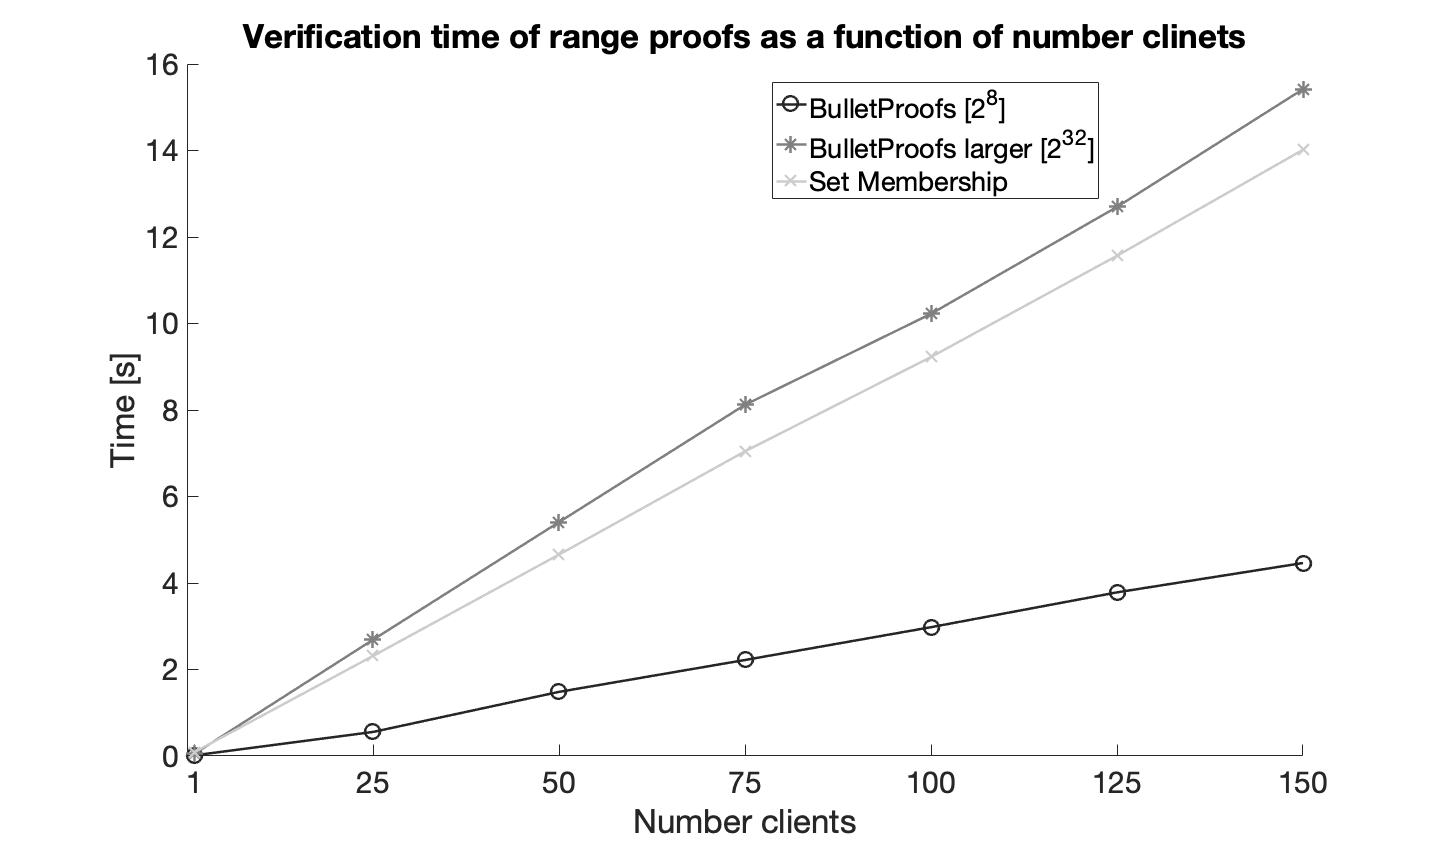
\includegraphics[width=\linewidth]{./figure/verification_nrClients.png}
\end{figure}


\begin{table}
\label{tab:BenchBP}
\caption{Timing in seconds for server and client verifiable-AHSS. Verfication of clients is done by usingBulletProofs}
\centering
\begin{tabular}{*{5}{c}}
\hline
    										&  \textbf{Executer}   & \multicolumn{3}{c}{\textbf{Time}}   		\\ 
    										& 								& Bullet proof  & signature based & Set membership \\	\hline
  GenerateShares 				&  client  					&   95 [$\mu$s]			 &96[$\mu$s]  &98 [$\mu$s]												\\ \hline 
  GenerateRangeProof  		&  clients  					&   53 [ms]				& 	241 [ms]	&66 [ms]			\\ \hline 
  PartialEval  						&  server  					&   78	[$\mu$s]				&72[$\mu$s]	 		&	71	 [$\mu$s]							\\ \hline 
  PartialProof 					&  server 					&   273[$\mu$s]						& 5249 [$\mu$s]			& 5255 [$\mu$s]				\\ \hline 
  FinalEval  						&  x  							&   689 [ns]						&655  [ns]				&			699  [ns]												\\ \hline 
  FinalProof  						&  x 							&   50	[$\mu$s]			&  114 [$\mu$s]	&				115 [$\mu$s]									\\ \hline 
  VerifyRP							&  x 							&   2979[ms]					&  &					9288 [ms]							\\ \hline 
  VerifyServers					&  x 							&   1672 [$\mu$s]					&		7990 [ms] 	&		7947 [$\mu$s]					\\ \hline 
\end{tabular}
 \end{table}

% VAHSS 
\chapter{Application in VAHSS}
\label{ch:VAHSS}
In this chapter, an application of the aggregated set membership proof is presented and evaluated. As discussed in chapter \ref{ch:intro}, VAHSS is an example where multiple data providers, henceforth denoted clients, participate. In this chapter first a construction of VAHSS  that verifies the servers computation is presented, then it is derived how to extend the verification to also include the clients. 
%The verification of clients requires each client to prove that the shared secret is in a predetermined allowed set or range.
Then different methods for verifying clients are compared. The comparison   mainly focuses on comparing aggregated signature-based set membership proof presented in Construction \ref{alg:ZKSM-Agg} with the state-of-the-art Bulletproofs for verification of clients to see how the runtime of the construction is affected.


\section{VAHSS}
\label{sec:VAHSS-HSS}
%Consider $n$ clients and $m$ servers, to simplify notation define the two sets $\mathcal{N}=\{1,...,n\}$ and $\mathcal{M} = \{1,...,m\}$. Let $c_i$ and $x_i$ for $i\in\mathcal{N}$ denote the clients (data providers) and their respective data. Denote the servers by $s_j$, where $\:j\in\mathcal{M}$.
The considered construction of VAHSS presented in \cite{SumItUp}, implemented and benchmarked in \cite{VAHSS}, makes use of homomorphic hash functions to verify the computations performed by servers.

%In this section the construction of the Verifiable Additive Homomorphic Secret Sharing (VAHSS), that this paper aim to extend is presented. The goal is to extend the VAHSS such that it in addition to  the verification of servers computations client are also verified to be honest. This will be done  by verifying that they do not provide false data. Different methods for verifying the data provided by the clients is explained in the next section.

%Before extending the VAHSS construction to additionally verify clients and combining it with the aggregated set membership proof introduced in the previous chapters. The VAHSS construction considered will be explained briefly. 

Assume that $n$ clients and $m$ servers participate in the VAHSS construction. The sets $\mathcal{N}=\{1,...,n\}$ and $\mathcal{M} = \{1,...,m\}$ are introduced to simplify notation. The clients are denoted $c_i$ for $i\in\mathcal{N}$, and their respective data $x_i$.  The servers in the construction are refereed to $s_j$ for $\:j\in\mathcal{M}$. 

Each client $c_i$ splits the secret $x_i$ into $m$ shares, denoted $\{x_{ij}\}_{j\in\mathcal{M}}$, such that $x_i=\sum_{j\in\mathcal{M}}x_{ij}$ and sends one share to each server. Each server $s_j$,  $j\in\mathcal{M}$, receives shares from all $n$ clients and computes and publishes the partial sum $y_j = \sum_{i\in\mathcal{N}} x_{ij} $. Then the final sum can be computed by any party by summing the public partial sums, which gives $y = \sum_{j\in\mathcal{M}} y_j = \sum_{j\in\mathcal{M}} \sum_{i\in\mathcal{N}} x_{ij} = \sum_{i\in\mathcal{N}} \sum_{j\in\mathcal{M}} x_{ij} =   \sum_{i\in\mathcal{N}}x_i$.

%For AHSS constructions, the idea is that each client splits their secret, $x_i$, into $m$ shares, denoted $x_{ij}$. The clients then sends one share to each server. The servers receives shares from all $n$ clients and computes the partial sum $y_j = \sum_{i\in\mathcal{N}} x_{ij} $ and publishes the result. The final sum can then be computed by any party by summing the public partial sums, this gives $y = \sum_{j\in\mathcal{M}} y_j = \sum_{j\in\mathcal{M}} \sum_{i\in\mathcal{N}} x_{ij} =  \sum_{i\in\mathcal{N}}x_i$. For VHASS construction in addition to AHSS a proof $\sigma$ that verifies that the partial sums $y_j=  \sum_{i=1}^n  x_{ij} $,  for all $j\in\mathcal{M}$, is generated and published. This allows any party to verify the correctness of the servers computations.

A proof $\sigma$ of the servers computations is obtained accordingly.  Each client $c_i$ publishes a checksum $\tau_i= g^{x_i+R_i}$, where $x_i$ is the secret hidden by the distributed shares and $R_i\in_R\mathds{F}$ is such that $R_n=\phi(p) \lceil \frac{\sum_{i=1}^{n-1}R_i}{\phi(p)}\rceil - \sum_{i=1}^{n-1}R_i $. Each server $s_j$ computes a partial proof $\sigma_j = g^{y_j}$.  Finally the verification is done by checking if $\prod_{j\in\mathcal{M}} \sigma_j = \prod_{i\in\mathcal{N}}\tau_i\wedge \prod_{i\in\mathcal{N}}\tau_i = g^y$.  If it holds the servers computations are proved to be correct. For a precise implementation and proof of correctness, security and verification the reader is refereed to the original paper about VAHSS \cite{SumItUp}.


\section{Client and Server VAHSS}
The VAHSS construction discussed in section \ref{sec:VAHSS-HSS} assumes honest clients and verifies the servers. This section extends the VAHSS construction to verify both the clients' input and the computations performed by the servers. First it is stated how to extend the VAHSS construction to additionally verify clients. Then a construction, using range proofs or set membership proofs, to verify clients is derived. It is then discussed how such a construction can be modified to use aggregated set membership proofs for verification of client' inputs. 

%If a range proof or set membership proof is included in the VAHSS construction then a potentially malicious clients can have a limited influence on the computed sum. Range proofs and set membership proofs force malicious input to still be part of a certain range or set. This leads to that the impact on the sum that a malicious client can have is bounded by the size of the range or by the elements in the set. 

% \subsection*{Verification of clients in VAHSS}
%In this section investigates how to combine the VHASS construction with a range proofs or set membership proofs.  Only range proofs and set membership proofs emanate from a Pedersen commitment hiding a secret is considered. 

\subsection*{Extending VAHSS to verify clients}
To ensure honest clients it is not sufficient to construct and perform a set membership proof and a VAHSS scheme separately. In such a protocol the verifier cannot be sure that the secret proven to be in the allowed set is the same as the secret hidden by the shares. The same principle holds considering range proofs. Therefore, a connection between the shares generated in the algorithm \textbf{ShareSecret} in the VAHSS construction and the secret hidden in a Pedersen commitment is desired. Proving that the sum of the shares is equal to the secret in a Pedersen commitment and then proving that the secret in the Pedersen commitment is in an allowed range or set convinces the verifier that the shares represent a secret that is in the allowed range or set. %The proof of the secret in the commitment is assumed to be a zero-knowledge range proof or zero-knowledge set membership proof of a secret in a Pedersen commitment.
%TODO fix: want to say general onlly
%Using the Pedersen commitment to link the VAHSS construction with a range proof or set membership proof, results in a general construction of a client and server VAHSS, compatible with any range proof or set membership proof of a secret in a Pedersen commitment.
% It is investigated if a Pedersen commitment can be included in the VAHSS construction, to obtain such a general construction of a client and server VAHSS 

%Publishing a Pedersen commitment of the secret itself does not provide any guarantee that it is the same secret that is hidden by the shares. It can also be seen that committing to the shares in Pedersen commitments does not ensure the verifier that the secret hidden in the shares are in the allowed set or range. This is since the individual shares themselves does not reveal information about the secret they are hiding. This leads to that there is not guarantee that proving a share belongs to the allowed range (or set) implies that the secret does and the other way assuming that the secret to a range (or set) does not imply that the shares does.

%Thus some trick to connect the secret in the shares to the secret in the Pedersen commitment must be derived. Therefore  that the aggregation of the partial proofs used in the VAHSS construction to prove the honesty of the servers will be used to connect the range proofs to the VAHSS construction.

In the VAHSS construction the clients publishes, in addition to the shares,  the checksums $\tau_i$ for the secrets $x_i$. Recall that the definition of the checksum is  $\tau_i=g^{x_i+R_i}$. The checksum $\tau_i$ can be interpreted as a Pedersen commitment, where $g=h$.

Hereafter, the clients compute and outputs the Pedersen commitments $\pi_i=g^{x_i}h^{R_i}$, instead of the previously computed checksums $\tau_i$.  Given a commitment $\pi_i$, the clients can construct a range proof or set membership proof of the committed secret. It remains to argue that this would ensure the verifier that the secret hidden by the shares is the same secret proved to be in the allowed range or set as for all $i\in\mathcal{N}$.


%Therefore the  checksum may be used as a Pedersen commitment in the construction of a range proof  or set membership proof. Formally the checksum is a Pedersen commitment where $g=h$. However if $g=h$ the computationally binding property of a Pedersen commitment would not hold since $log_g(h)=log_g(g)=1$ which leads to that the left hand side in equation \eqref{eq:pedersen_binidng} is equal to $1$. Therefore to construct two commits $\mathds{E}(x,R)$ and $\mathds{E}(x',R')$ such that $\mathds{E}(x,R) = \mathds{E}(x',R')$ but $x\neq x'$ it is sufficient to solve solve for $x'$ in, 
%\begin{align*}
%R'-R = x-x'\:mod \:p .
%\end{align*}
%In other words it is straightforward to create a false commitment hence also a false range proof and set membership proof.

%TODO use set instead of range och fixa
Assume that client $c_k$ commits to the value $\hat{x}_k$ in the Pedersen commitment $\pi_k$, constructs the shares $\{x_{kj}\}_{j\in\mathcal{M}}$ such that $x_k = \sum_{j\in\mathcal{M}}x_{kj} \neq \hat{x}_k$ and  generates a ZKP that $\hat{x}_k$ belongs to the set $\Phi$ or range $[a,b]$. Since $x_k\neq\hat{x}_k$ this does not necessarily imply that  the secret hidden by the shares belongs to the range or set. Then  $\prod_{i=1}^m \pi_i \neq g^y$  and thereby the verification of servers does not succeed. Thus it has to hold that $x_k= \hat{x}_k$ for the protocol to succeed and any cheating client is detected. It is not possible to determine which party cheated and more precisely not even if the cheating party was a client or a server. 

\begin{Remark}
\label{thm:VAHSS_RP_CSV}
\vspace{10pt}
The correctness, security and verifiability requirements of a VAHSS construction holds after replacing the checksums $\tau_i= g^{x_i+R_i}$ with a Pedersen commitment $\pi_i= g^{x_i}h^{R_i}$ in the VAHSS construction, \cite{SumItUp}. 

Additionally if a range proof or set membership proof, denoted $\Sigma_i$, that satisfies the soundness, completeness and zero-knowledge requirements of zero-knowledge proofs is constructed of the secret $x_i$ in the Pedersen commitment $\pi_i$, for all clients $c_i$ in the VAHSS construction. Then any PPT adversary $\mathcal{A}$ who can modify the Pedersen commitments $\pi_i$  to any $\pi_i^{'} \:\forall  i\in T$, where $T$ is the set of corrupted clients, has a negligible probability of choosing a commitment $\pi_i^{'}$ such that verification of all the proofs $\Sigma_i$ and the VAHSS validates true.
%\begin{itemize}
 %\item \textbf{Verifiability Servers}  Let $\mathcal{A}$ denote any PPT  adversary and $T$ denote the set of corrupted servers with $T\leq m$. Note that if $|T|=m$, the verifiability property holds but not the security property. The verifiability property requires that any $\mathcal{A}$ who can modify the input shares to all servers $s_j\in T$ can cause a wrong value to be excepted as $y=f(x_1,...,x_n)$ with negligible probability.  
 %\item  \textbf{Verifiability Clients} 
%\end{itemize} 
\end{Remark}
%TODO fix proof before hand in to Seminar 2
\textbf{Proof of remark:}
The remark follows from that  replacing  $\tau_i$ with $\pi_i$ for $i=1,...,n$, it still holds that:
\begin{align*}
&\prod_{i\in\mathcal{N}} \pi_i = \prod_{i\in\mathcal{N}} g^{x_i}h^{R_i} = g^{\sum_{i\in\mathcal{N}} x_i}h^{\sum_{i\in\mathcal{N}} R_i} = g^{y} h^{ \phi(N)\big\lceil \frac{\sum_{i=1}^{n-1}R_i}{\phi(N) }\big\rceil} = g^y \\
&\text{Thereby it follows that: } \prod_{i\in\mathcal{N}}^n \tau_i = \prod_{i\in\mathcal{N}} \pi_i.
\end{align*}
Further the Pedersen commitment is perfectly hiding as well as computationally binding and thus it follows that the requirements are still fulfilled. 

From the soundness of range proofs and set membership proofs, and the above argument that the secret hidden in the commitment $\pi_i$ must be the same as the secret obtained by combining the the shares $\{x_{ij}\}_{j\in\mathcal{M}}$ for all $i=\mathcal{N}$, it follows that any adversary who can modify the commitments $\pi_i$ has a negligible probability of doing so such that the proofs $\Sigma_i$ and the VAHSS construction validates true. $\quad \square$

\begin{comment}
The correctness follows from the correctness of range proofs and by proving that $\sigma= \prod_{i=1}^n \pi_i \:\bigwedge\: \prod_{i=1}^n \pi_i = \mathcal{H}(y)$. Both $y$ and $\sigma$ are the same as in Construction \ref{alg:VAHSS-HSS}, hence by construction:
\begin{align}
    \label{eq:y=sum(x_ij)}
    y = \sum_{j=1}^m y_j= \sum_{j=1}^m \sum_{i=1}^n \lambda_{ij}p_i(\theta_{ij}) = \sum_{i=1}^n \overbrace{ \Big (\sum_{j=1}^m \lambda_{ij}p_i(\theta_{ij}) \Big)}^{ p_i(0)} = \sum_{i=1}^n p_i(0) = \sum_{i=1}^n x_i,
\end{align}
and for $\sigma$ it holds that:
\begin{align*}
    \sigma = \prod_{j=1}^m \sigma_j = \prod_{j=1}^m g^{y_j} = g^{\sum_{j=1}^my_j} =g^y = \mathcal{H}(y)
\end{align*}
For the $\pi_i$, whose construction has been modified compared to $\tau_i$ in  Construction\ref{alg:VAHSS-HSS}, thus it follows that:
\begin{align*}
    &\prod_{i=1}^n \pi_i = \prod_{i=1}^n \mathds{E}(x_i,R_i)= \prod_{i=1}^n g^{x_i}h^{R_i} = g^{\sum_{i=1}^n x_i } h^{\sum_{i=1}^n R_i} \overset{\eqref{eq:y=sum(x_ij)}}{=} g^y h^{\sum_{i=1}^{n-1} R_i+R_n} = \\ 
    &= g^y h^{ \phi(N)\big\lceil \frac{\sum_{i=1}^{n-1}R_i}{\phi(N) }\big\rceil} = g^y = \mathcal{H}(y) 
\end{align*}

The proof of security argument for malicious servers given in \cite{SumItUp} is still sufficient since the Pedersen commitment is perfectly hiding and computationally binding and that the range proofs are zero-knowledge. The security argument for malicious clients follows from the soundness of the range proof and that the secret hidden in the commitment has to be the same as the secret in the shares, as argued above. . 

The proof of \textit{\textbf{Verifiability Severs}} is the same as the proof given in  in \cite{SumItUp}, except that the commitments $\pi_i$ replaces the checksums $\tau_i$.  \textit{\textbf{Verifiability Clients}} follows from the properties of the range proof.
\end{comment}
%\end{proof}

\subsection*{Verifying clients using set membership proofs or range proofs}
A VAHSS where clients are verified by publishing range proofs or set membership proofs is presented in Construction \ref{alg:VAHSS-HSS-RP}.  In order to clarify the changes made to extend the construction to  verify clients, the differences to the VAHSS construction presented in \cite{SumItUp} are pointed out.

The algorithms \textbf{ShareSecret} and \textbf{Verify} has been modified,  and the algorithms \textbf{ProveSecret} and \textbf{GenerateCommitment} have been added. More precisely, the algorithm \textbf{ShareSecret} does not output the checksum $\tau_i$, instead the Pedersen commitment $\pi_i$ is computed in the algorithm \textbf{GenerateCommitment}. The algorithm \textbf{ProveSecret} constructs a set membership proof or range proof denoted $\Sigma_i$ given the commitment $\pi_i$. 
%The precise construction of the range proof or set membership proof that is used does not affect the rest of Construction \ref{alg:VAHSS-HSS-RP}, as long as it originates from a Pedersen commitment.
 In addition to the steps of the algorithm \textbf{Verify} in the VAHSS construction presented in \cite{SumItUp}, the algorithm \textbf{Verify} also validates the proofs $\Sigma_i$ for all $i\in\mathcal{N}$.
 
%The algorithm  \textbf{GenerateCommitment} can be included in either \textbf{ShareSecret}  or \textbf{RangeProof} instead of being viewed as a separate algorithm. In the implementation discussed later the commitment is generated while constructing the range proof and not explicitly. 

The algorithms \textbf{GenerateCommitment} and \textbf{ProveSecret} are executed by the clients and the other algorithms are executed by the same party as in the  VAHSS construction in \cite{SumItUp}. 

Remark \ref{thm:VAHSS_RP_CSV}  implies that Construction \ref{alg:VAHSS-HSS-RP} satisfies the correctness, security and verification requirements for a VAHSS construction and that the verification of clients' input satisfies the completeness, soundness and zero-knowledge requirements of the considered range proofs or set membership proofs.

%In the VAHSS Construction \ref{alg:VAHSS-HSS} the verifiability property includes verification of the servers. In this section this will be extended to also include the clients. The value $\pi_i$ published by the clients will be modified into a Pedersen commitment on the form $\pi_i = g^{x_i}h^{R_i}$, remember $\pi_i=g^{x_i+R_i}$ in the original construction presented in \cite{SumItUp}. The clients will apart from the previous commitments  also construct and publish a range proof for $\pi_i$. This allows any verifier to apart from verifying the servers also verify that the secret shared by the clients is in an certain range.  

%Given this construction the correctness, security and verification requirements for the server verifiable AHSS presented in \cite{SumItUp} is still fulfilled  that should be fulfilled is redefined below.  The difference to the requirements for the server verifiable AHSS is that additional demands for the clients behaviour is included. 

\begin{comment}
\begin{itemize}
    \item \textbf{Correctness} It must hold that Pr$\Big[\textbf{Verify}(\{\pi_i\}_{i\in\mathcal{N}},\sigma,y,\{\Sigma_i\}_{i\in\mathcal{N}})=1\Big]=1$. This means that with probability $1$ the output $y$ from \textbf{FinalEval} is accepted given all parties (clients and servers) where honest and the protocol were executed correctly.
    \item \textbf{Security} 
    			\begin{itemize}
    						\item \textbf{Malicious Servers } The construction should satisfy the same security argument as the VAHSS-HSS construction in \cite{SumItUp}.
    						%Let $T$ define the set of corrupted servers such that $|T|<m$, i.e at 					least one server is honest.  										Denote a PPT adversary by $\mathcal{A}_1$ and let the Adv$(1^			\lambda,\mathcal{A},T):= \text{Pr}[b' = b]-1/2$ be the advantage 										of $\mathcal{A}=\{\mathcal{A}_1,\mathcal{D}\}$ in guessing $b$ in the following experiment:
    							%		\begin{enumerate}
       						%				 \item The adversary $\mathcal{A}_1$ gives $(i,x_i,x_i')$ to the challenger, where $i\in[n], x_i\neq x_i'$ and $|x_i|=|x_i'|$.
        						%				\item The challenger picks a bit $b\in\{0,1\}$ uniformly at random chooses and computes $\textbf{ShareSecret}(1^\lambda,i,																\hat{x}_i) = (\hat{\text{share}}_{i1},...,\hat{\text{share}}_{im},\tau_i)$, where $\hat{\textbf{x}}_i$ is  such that $\hat{x}_i = 																\begin{cases}x_i, \text{ if } b=0 \\ x_i' \text{ else} \end{cases}$. 
        					%					\item Given the shares from the corrupted servers T and $\hat{\tau}_i$ the adversary distinguisger outputs a guess 																			$b'\xleftarrow[]{}\mathcal{D}((\hat{\text{share}_{ij}})_{j|s_j\in T},\hat{\tau}_i)$.
   									% \end{enumerate}
    							%		A VAHSS-construction is $t$-secure if for all $T\subset \{s_1,...,s_m\}$ with $|T|<t$ it holds that Adv$(1^\lambda,\mathcal{A},T)<												\varepsilon(\lambda)$ for some negligible $\varepsilon(\lambda)$.
  					  \item \textbf{Malicious Clients}  Since the construction does not clarify the exact range proof used, the security argument is refereed to the original papers for the used range proof and by proving that the secret hidden by the Pedersen commitments is the same as the secrets in the shares. 
   		 \end{itemize} 
 	\item \textbf{Verifiability} 
 			\begin{itemize}
 						\item \textbf{Verify Servers }Let $\mathcal{A}$ denote any PPT  adversary and $T$ denote the set of corrupted servers with $T\leq m$. The verifiability 							property requires that any $\mathcal{A}$ who can modify the input shares to all servers $s_j\in T$ can cause a wrong value to be excepted as 							$y=f(x_1,...,x_n)$ with negligible probability.   
 						\item \textbf{Verify Clients} Let $\mathcal{A}$ denote any PPT adversary and $T$ denote the set of corrupted clients. The verifiability property requires that any $\mathcal{A}$ who can modify the Pedersen commitments $\pi_i$  to any $\pi_i^{'} \:\forall  i\in T$ has a negligible probability at choosing a commitment $\pi_i^{'}$ such that Verify$( \{\pi^{'}_i\}_{i\in\mathcal{N}},x,y)=1$.
 			\end{itemize} 
\end{itemize}
\end{comment}

\begin{algorithm}
\caption{\textbf{: Client and Server Verifiable additive homomorphic secret sharing}}

\textbf{Goal:} Compute the sum $y = \sum_{i=1}^n x_i$. The values $x_i$ are kept secret. The servers computations and the clients shared values are verified. 
\vspace{2pt}\hrule\vspace{2pt}
\begin{itemize}
 \item\textbf{ShareSecret $(1^\lambda,i,x_i) \mapsto \{x_{ij}\}_{j\in\mathcal{M}}$} \\
Pick uniformly at random the coefficients, $\{a_i\}_{i\in\{1,..,t\}}\in_R\mathds{F}$ and define a $t$-degree polynomial $p_i$ to be on the form $p_i(X) = x_i + a_1X+...+a_tX^t$. Put the shares $x_{ij}=\lambda_{ij}p_i(\theta_{ij})$ for $j\in\mathcal{M}$.  The parameters $\theta_{ij}$ and Lagrange coefficients $\lambda_{ij}$ are chosen such that $ p_i(0) = \sum_{j=1}^m \lambda_{ij}p_i(\theta_{ij})$.
Output $\{x_{ij}\}_{j\in\mathcal{M}}$.

\item\textbf{GenereteCommitment$(1^\lambda,i,x_i) \mapsto \pi_i$ }\\
Let $R_i\in\mathds{F}$ be the output of a PRF such that $R_n\in \mathds{F}$  satisfies $R_n = \phi(N)\lceil \frac{\sum_{i=1}^{n-1}R_i}{\phi(N)}\rceil- \sum_{i=1}^{n-1}R_i $. Compute and output $\pi_i = \mathds{E}(x_i,R_i)= g^{x_i}h^{R_i}$.

\item\textbf{ProveSecret $(pp,x_i,\pi_i) \mapsto \Sigma_i$}\\
Construct a range proof or set membership proof, denoted $\Sigma_i$, for the Pedersen commitment $\pi_i$ of the secret $x_i$, on the  range $[a,b]$ or a set $\Phi$. All required public parameters, $pp$, needed to  construct the proof $\Sigma_i$ is assumed to be pre-shared and known by all parties.
\item\textbf{PartialEval $(j,\{x_{ij}\}_{i\in\mathcal{N}})\xrightarrow[]{}y_j$}\\
Compute and output $y_j = \sum_{i=1}^n x_{ij}$.

\item\textbf{PartialProof $(j,\{x_{ij}\}_{i\in\mathcal{N}})\xrightarrow[]{}\sigma_j$}\\
Compute and output $\sigma_j = \prod_{i=1}^n g^{x_{ij}} =  g^{\sum_{i=1}^n x_{ij}}= g^{y_j}=\mathcal{H}_1(y_j)$.

\item\textbf{FinalEval $(\{y_j\}_{j\in\mathcal{M}})\xrightarrow[]{}y$}\\
Compute and output $y = \sum_{j=1}^m y_{j}$.

\item\textbf{FinalProof $(\{\sigma_j\}_{j\in\mathcal{M}})\xrightarrow[]{}\sigma$}\\
Compute and output $\sigma = \prod_{j=1}^m \sigma_j = \prod_{j=1}^m g^{y_{j}} =  g^{\sum_{j=1}^m y_{j}}= g^{y}=\mathcal{H}_1(y)$.

\item\textbf{Verify $(\{\pi_i\}_{i\in\mathcal{N}},x,y,\{\Sigma_i\}_{i\in\mathcal{N}})\xrightarrow[]{}\{0,1\}$}\\
Compute and output $\sigma= \prod_{i=1}^n \pi_i \wedge \prod_{i=1}^n \pi_i = \mathcal{H}_1(y)\wedge \{\textbf{VerifyProof}( \Sigma_i) \}_{i\in\mathcal{N}}$. $\textbf{VerifyProof}$ is the verification algorithm of  the  proofs $\{\Sigma_i\}_{i\in\mathcal{N}}$.
\end{itemize}
\label{alg:VAHSS-HSS-RP}
\end{algorithm}

\subsection*{Verifying clients using aggregated set membership proofs}
Construction \ref{alg:VAHSS-HSS-RP-Agg} describes a client and server VAHSS compatible with aggregated set membership proofs for verification of clients. The algorithms in Construction \ref{alg:VAHSS-HSS-RP-Agg} are the same as in Construction \ref{alg:VAHSS-HSS-RP} except that the algorithm \textbf{PartialAggregate} is introduced and the algorithm \textbf{Verify} is modified. 

The algorithm \textbf{PartialAggregate} is run by all aggregating parties in the set $\mathcal{K}$ and the algorithm \textbf{Verify} is modified such that it verifies the aggregated proofs instead of the individual clients' proofs.

If the server computing the partial sums $y_j$ are responsible for aggregation of the clients set membership proofs, then no new parties are introduced to the VAHSS construction to aggregate the proofs.  Then the set $\mathcal{K}$ is equal to $\mathcal{M}$ in construction \ref{alg:VAHSS-HSS-RP-Agg}. 
 
For aggregation in Construction \ref{alg:VAHSS-HSS-RP-Agg} to be sound, the aggregation must either be performed by a trusted party or split between at least two aggregating parties. 

If the aggregation is performed by an untrusted party, this party can cheat in the aggregation of the proofs, by exploiting that the sum $y$ can be computed once the servers have performed the algorithm \textbf{PartialEval} and that  $h^{\sum_{i\in\mathcal{N}} R_i } =1 \: \text{mod}\:  \phi(p)$. Note that this induces that  the assumptions of Theorem \ref{thm:aggrgeation} are not fulfilled, since the aggregation party has additional knowledge beyond the input to the algorithm \textbf{Aggregate} and the commitments $\{C_i\}_{i\in\mathcal{S}}$. %Although the individual secrets are unknown, it is possible to cheat when constructing the aggregated proof $\Sigma_a$, by using the fact that $y=\sum_{i\in\mathcal{N}}x_i, h^{\sum_{i\in\mathcal{N}}R_i}$ are known. 
Since $y$ is known to the aggregating party, the aggregated proof $\Sigma_a$ can be constructed as, $D_a=C^{k+c}, z_{R_a} = k\phi (N)$ and $z_{x_a} = k y$, where $y= \sum_{i\in\mathcal{N}} x_i$ and $k\in_R \mathds{F}$. Then it follows that:
\begin{align*}
D_a &= C^{k+c}= \big( g^ { k \sum_{i=1}^n x_i } h^{ k  \sum_{i=1}^n R_i ) } \big)   \big( g^{ (  \prod_{i=1}^n c_i ) \sum_{i=1}^n x_i ) } h^{ ( \prod_{i=1}^n c_i ) \sum_{i=1}^n R_i ) } \big)   \\
 C^c h^{z_{R_a}}g^{z_{x_a}} &= C^c h^{k \phi (N) } g^{k y} =  \big( g^{ (  \prod_{i=1}^n c_i ) \sum_{i=1}^n x_i ) } h^{ ( \prod_{i=1}^n c_i ) \sum_{i=1}^n R_i ) } \big) h^{k\phi (N)} g^{ky}\\
= &  \big( g^{ (  \prod_{i=1}^n c_i ) \sum_{i=1}^n x_i ) } h^{ ( \prod_{i=1}^n c_i ) \sum_{i=1}^n R_i ) } \big)g^ { k y} h^{ k  \phi(N)\lceil \frac{\sum_{i=1}^{n-1}R_i}{\phi(N)}\rceil ) }\\
& \implies D_a = C^ch^{z_{R_a}}g^{z_{x_a}}.
\end{align*}

It has been shown that if one party aggregating all clients' set membership proofs the aggregation is not sound, since the aggregated proof can be constructed such that it validates true without proving the statement in equation \ref{eq:SMagg_statement}. 
%Further it is seen that  it is possible for such an aggregating party to  cheat and provide an aggregated proof that  verifies true without the statement in equation \eqref{eq:SM_statement} being true.

If multiple parties aggregates subsets of the proofs, the assumptions in Theorem \ref{thm:aggrgeation} holds,  this follows from that the sum of the secrets and random values are unknown considering any true subset of the clients. 

Under the assumption that the aggregation is sound, Remark \ref{thm:VAHSS_RP_CSV} applies to Construction \ref{alg:VAHSS-HSS-RP-Agg}. Thereby, if the aggregation is performed by a trusted party or is split between at least two independent aggregating parties, Construction \ref{alg:VAHSS-HSS-RP-Agg} satisfies the correctness, security and verification requirements for a VAHSS construction and the verification of clients' input satisfies the completeness, soundness and zero-knowledge requirements of the considered range proofs or set membership proofs. 

\begin{algorithm}
\caption{\textbf{: Client and Server Verifiable additive homomorphic secret sharing}}

\textbf{Goal:} Compute the sum $y = \sum_{i=1}^n x_i$. The values $x_i$ are kept secret. Servers computations and clients shared values are verified. 
\vspace{2pt}\hrule\vspace{2pt}
\begin{itemize}
 \item\textbf{ShareSecret $(1^\lambda,i,x_i) \mapsto \{x_{ij}\}_{j\in\mathcal{M}}$} \\
Pick uniformly at random the coefficients, $\{a_i\}_{i\in\{1,..,t\}}\in_R\mathds{F}$ and define a $t$-degree polynomial $p_i$ to be on the form $p_i(X) = x_i + a_1X+...+a_tX^t$. Put the shares $x_{ij}=\lambda_{ij}p_i(\theta_{ij})$ for $j\in\mathcal{M}$.  The parameters $\theta_{ij}$ and Lagrange coefficients $\lambda_{ij}$ are chosen such that $ p_i(0) = \sum_{j=1}^m \lambda_{ij}p_i(\theta_{ij})$.
Output $\{x_{ij}\}_{j\in\mathcal{M}}$.

\item\textbf{GenereteCommitment$(1^\lambda,i,x_i) \mapsto \pi_i$ }\\
Let $R_i\in\mathds{F}$ be the output of a PRF such that $R_n\in \mathds{F}$  satisfies $R_n = \phi(N)\lceil \frac{\sum_{i=1}^{n-1}R_i}{\phi(N)}\rceil- \sum_{i=1}^{n-1}R_i $. Compute and output $\pi_i = \mathds{E}(x_i,R_i)= g^{x_i}h^{R_i}$.

\item\textbf{ProveSecret $(pp,x_i,\pi_i) \mapsto \Sigma_i$}\\
Construct a range proof or set membership proof, denoted $\Sigma_i$, for the Pedersen commitment $\pi_i$ of the secret $x_i$, on the  range $[a,b]$ or a set $\Phi$. All required public parameters, $pp$, needed to  construct the proof $\Sigma_i$ is assumed to be pre-shared and known by all parties.
\item\textbf{PartialEval $(j,\{x_{ij}\}_{i\in\mathcal{N}})\xrightarrow[]{}y_j$}\\
Compute and output $y_j = \sum_{i=1}^n x_{ij}$.

\item\textbf{PartialProof $(j,\{x_{ij}\}_{i\in\mathcal{N}})\xrightarrow[]{}\sigma_j$}\\
Compute and output $\sigma_j = \prod_{i=1}^n g^{x_{ij}} =  g^{\sum_{i=1}^n x_{ij}}= g^{y_j}=\mathcal{H}_1(y_j)$.

\item \text{\textbf{PartialAggregate} $(pp,k,\mathcal{S}_k, \{\Sigma_i\}_{i\in\mathcal{S}_k} ) \xrightarrow[]{} \Sigma_{a_k}$} \\
On the input $\{ \Sigma_i \}_{i\in\mathcal{S}_k}$ where $\mathcal{S}_k\subseteq\{1,...,n\}$, the set of proofs is aggregated according to the algorithm \textbf{Aggregate} in Construction \ref{alg:ZKSM-Agg} and  aggregated proof $\Sigma_{a_k}$ is published. 

\item\textbf{FinalEval $(\{y_j\}_{j\in\mathcal{M}})\xrightarrow[]{}y$}\\
Compute and output $y = \sum_{j=1}^m y_{j}$.

\item\textbf{FinalProof $(\{\sigma_j\}_{j\in\mathcal{M}})\xrightarrow[]{}\sigma$}\\
Compute and output $\sigma = \prod_{j=1}^m \sigma_j = \prod_{j=1}^m g^{y_{j}} =  g^{\sum_{j=1}^m y_{j}}= g^{y}=H(y)$.

\item\text{ \textbf{Verify} $(\{\pi_i\}_{i\in\mathcal{N}},x,y,\{\Sigma_{a_k} \}_{k\in\mathcal{K}})\xrightarrow[]{}\{0,1\}$}\\
Compute and output $\sigma= \prod_{i=1}^n \pi_i \wedge \prod_{i=1}^n \pi_i = H(y)\wedge \{\textbf{VerifyProof}(\Sigma_{a_k})\}_{k\in\mathcal{K}}$. $\textbf{VerifyProof}$ is the verification algorithm in Construction \ref{alg:ZKSM-Agg}.
\end{itemize}
\label{alg:VAHSS-HSS-RP-Agg}
\end{algorithm}


%For the VAHSS construction this can be implemented by letting the server, which computes the partial sums, aggregate different subset of the clients set membership proofs. 

 %And if the set set of aggregating parties $\mathcal{K}$ consist of one element and $\mathcal{S}_k  = \mathcal{N}$ the partial aggregation would correspond to a full aggregation, and Construction \ref{alg:VAHSS-HSS-RP-Agg} would describe the aggregated client and severs VAHSS construction for a single trusted aggregating party. 

%To conclude, if the aggregation is not assumed to be performed by a trusted party then the characteristics of the VAHSS construction all set membership proof cannot be aggregated by a single party. Thus then the aggregation must the split between atleast two parties.  


%The main result obtained is that it is possible to extend the VAHSS construction presented in Construction \ref{alg:VAHSS-HSS} such that honesty of the clients is verified. The proposed verification of clients ensure the verifier that all clients shared secrets belonging to a pre-specified allowed range or set. Given the existence of such a range or set, each client provides a zero-knowledge proof that their secret is in the range or set. The verification algorithm for the client and sever verifiable AHSS, compared to the algorithm in Construction \ref{alg:VAHSS-HSS}, is extended to verify all range proof or set membership proofs published by the clients. This leads to that the verifier after having performed the verification is convinced that all secrets in the summation belongs to the allowed range or set, and that all servers computations was done correctly. 

%All constructions examined to provide a proof that a secret is in an allowed range or set, assumes that there exists pre-published Pedersen commitment of the secret and proves the statement for the secret in the commitment.  Exploiting this similarity between various range proofs and set membership proofs when combining them with a VAHSS lead to that a general methodology for including verification of clients in the VAHSS construction. The proposed client and server VAHSS in Construction \ref{alg:VAHSS-HSS-RP} is independent of the construction used to prove that a statement in in an allowed range or set, given that it is proved for a secret in a Pedersen commitment. Note that it is implicitly assumed that 
%construction can provide a proof for the desired range or set and that
%the algorithm for construction of the proof and verifying of the proof are compatible.

%Theorem \ref{thm:VAHSS_RP_CSV} states the correctness, security and verification of Construction \ref{alg:VAHSS-HSS-RP}. It is seen that the extending the VHASS with a verification of the clients preserves the correctness, security and verification requires for the VAHSS. Moreover the verifier is convinced that the secrets shared by the clients belongs to an allowed range or set. 


\section{Implementation}
\label{sec:implementation}
%TODO what to include here? 
% Discuss translation to Golang. 
An implementation of Constructions \ref{alg:VAHSS-HSS-RP} and \ref{alg:VAHSS-HSS-RP-Agg} is obtained to investigate the proposed clients and server VAHSS in a practical setting and comparing the runtime for different methods for verifying clients.
%To provide an implementation of Construction \ref{alg:VAHSS-HSS-RP} and \ref{alg:VAHSS-HSS-RP-Agg} the algorithms constructing a VAHSS  are combined with the algorithms to prove and verify clients.  Bulletproofs, aggregated and not aggregated signature-based set membership proofs are the considered methods for verifying clients.  %is provided written in Golang. 

%Remark that this construction is written without specifying which range proof that is used, and works for all different range proofs that provides a proof for a Pedersen commitment, which is true for all range proof discussed above.
 %From the prototype analysis given above it is clear that Bulletproofs is faster than signature-based range proof. Considering the aggregation possibility for signature based range proofs, Construction \ref{alg:VAHSS-HSS-RP} will be implemented using all three considered proofs to ensure honest clients. 
 
%  all three constructions will hence be used to implement the client and server verifiable additive homomorphic secret sharing construction \ref{alg:VAHSS-HSS-RP}. 

Bulletproofs, aggregated and non-aggregated signature-based set membership proofs implemented in Golang are publically available on Github, \cite{Git:RP} \cite{Git:mycode}. The VAHSS construction implemented in both python and C++,  is available at \cite{Git:python_vahss} and \cite{Git:C_vahss} respectively. 

To implement Construction \ref{alg:VAHSS-HSS-RP} and \ref{alg:VAHSS-HSS-RP-Agg},  the VAHSS algorithms need to be callable from the same programs as the algorithms for Bulletproofs, signature-based set membership proofs and aggregated signature-based set membership proofs. The VAHSS algorithms have been translated to Golang, to solve the problem of having the implementations written in different programming languages. The implementation is available at \cite{Git:mycode}.

To provide an implementation of Construction \ref{alg:VAHSS-HSS-RP} and \ref{alg:VAHSS-HSS-RP-Agg} besides translating the VAHSS code to Golang the implementations have also been slightly modified. The VAHSS construction has as discussed above been adjusted such that it considers a Pedersen commitment $\pi_i$ instead of the checksum $\tau_i$. The implementations of Bulletproofs, signature-based set membership proofs and aggregated signature-based set membership proofs have also been adjusted to be compatible with the VAHSS algorithms. These adjustments are merely to merge the constructions and does not change the semantics of the constructions. The modified implementations are available at \cite{Git:mycode}.


% To achieve this one of the two following modifications needs to be done. The first alternative is to \texit{wrap} the code from one programming language such that it can be compiled and used by another programming language. This would then mean to either write a wrapper for Go code such that it can be interpreted by a C++ (or Python) compiler, or alternatively wrap the  CC++ (or Python) code such that it can be interpreted by a Go compiler. The second alternative is to translate the VAHSS implementation into the same language as the Bulletproofs, signature-based range proof and set membership proof or the other way around. 

%The first alternative appears to be a simpler approach hence this is first tested. In 2016 \textit{cgo} was released which enables calling C functions from Go code. 
%The Go command \textit{cgo} enables Go packages to call C code. TODO...

%Instead consider the second alternative, that translating the code of one of the implementations such that all code is available in the same programming language. Since the VAHSS construction is  shorter than the two range proofs and the set membership proof all together, the VAHSS code was converted to Go.


%Besides translating the VAHSS implementations to Go a small adjustments of the already existing Go implementations of the range proofs and set membership proof  had to be done to merge with the VAHSS construction. This adjustment are merely to merge the codes and does not change the semantics of the range proofs. What has been  modified is that the randomness used in the Pedersen commitments in the range proof must be chosen such that $R_n = \phi(N)\lceil \frac{\sum_{i=1}^{n-1}R_i}{\phi(N)}\rceil- \sum_{i=1}^{n-1}R_i$, hence is is regarded as input to the proof constructions.The full code for combination of range proofs (or set membership proofs) and VAHSS is available at Git \ref{Git:MyCode}. 

%Just as in construction \ref{alg:VAHSS-HSS-RP} the implementation of the code aims to be  general, such that all three concerned range proofs can be used to verify clients honesty and the merge of the range proof to the VAHSS construction is the same for all range proofs. However note that although the construction does not specify which range proof that is used the implementation does due o the choice of underlying group in the set up, the signature-based range proofs and set membership proof uses pairing friendly elliptic curve groups in the implementation which is not the case for Bulletproofs. This leads to minor modifications of the implementation to adapt to range proofs and set membership proofs.
\subsection*{Implementation parameters}
The finite field $\mathds{F}$ is generated by a prime of size $256$-bit.

The number of servers is set to $5$, $|\mathcal{M}|=5$,  and the number of clients to $100$, $|\mathcal{N}|=100$.  The set of aggregation parties $\mathcal{K}$ is assumed to consist of a single party, meaning that $|\mathcal{K}|=1$.

Remark that the trade-off between runtime for aggregation and verification depending on the number of aggregation parties is presented in section \ref{sec:tradeoff}.  The result presented there translates directly to the runtime of the aggregation and the verification of clients in a server and client VAHSS.  Thereby, although $|\mathcal{K}|=1$ in this section the runtime considering multiple aggregating parties can be obtained by studying the results presented in chapter \ref{ch:results}.

The range is set to $[18,200]$ for the implementation of Bulletproofs, and thus the upper bound of the Bulletproof is set to $2^n$, where $n=8$. The size of the set $\Phi$ is put to the length of the range, $|\Phi|=200-18 = 182$, for both the aggregated and not aggregated signature-based set membership proofs. 

A final remark about the implementation is that its purpose is to test the above-proposed constructions and provide runtime evaluations, the code has not been tested enough to be considered as a secure implementation.



% runtime is important
% not aggregation here 
%This paper has studied three different constructions possible to combine with a VAHSS to verify clients. In the runtime comparison of these three constrictions, seen in Table \ref{tab:runtime}, it was noted that the set membership and Bulletproofs where notable faster than the signature-based range proof. Further it has been discussed that the set membership proof can be used a larger area of applications. This is due to that it proves membership of a sets which are more flexile than ranges. 

%Although the discussion above is favourable towards Bulletproofs and set membership proofs,  Construction \ref{alg:VAHSS-HSS-RP} has be implemented considering Bulletproofs, set membership proofs and signature-based range proofs. The runtime is consequently presented for all three combinations. This is also motivated by completeness of the comparison. 

\section{Prototype analysis}
%The implementation of Constructions \ref{alg:VAHSS-HSS-RP} and \ref{alg:VAHSS-HSS-RP-Agg}, using different construction to verify clients, are benchmarked to provide runtime results. The runtime results are used to compare the different constructions for verifying clients.

%Combining the VAHSS with a verification of clients, as done in Construction \ref{alg:VAHSS-HSS-RP} and \ref{alg:VAHSS-HSS-RP-Agg}, resulted in a constructions where the VAHSS algorithms are run almost in parallel to the algorithms for a range proofs or set membership proofs. The interaction between the two constructions is minimal and appears only in the verification.  Consequently it can be expected that the runtime for the different algorithms in Construction \ref{alg:VAHSS-HSS-RP} and \ref{alg:VAHSS-HSS-RP-Agg} are almost the same as the runtime for the algorithms for them in individual constructions, i.e VAHSS and range proofs or set membership proofs.

%For example the algorithms  \textbf{ShareSecret}, \textbf{PartialEval} run completely independent of the algorithm \textbf{RangeProof} in Construction \ref{alg:VAHSS-HSS-RP} and \ref{alg:VAHSS-HSS-RP-Agg}, resulting in that they are almost identical to the algorithms in the original VAHSS construction, \cite{SumItUp}. Thus the runtime for the algorithms are likely to comparable with the results given in \cite{VAHSS}. The same hold the other way around, that the algorithm \textbf{RangeProof} is likely to be comparable to previous runtime results, \cite{RANGE-SET}. 

%Smaller adjustment has been made to the algorithms due to combining and hence the runtime for all algorithms in the  the client and server VAHSS in evaluated.  

The runtime for the algorithms in Construction \ref{alg:VAHSS-HSS-RP} and \ref{alg:VAHSS-HSS-RP-Agg} is presented in Table \ref{tab:BenchBP}. Construction \ref{alg:VAHSS-HSS-RP} is benchmarked considering two different constructions for verifying clients:  Bulletproofs and signature-based set membership proofs. Construction \ref{alg:VAHSS-HSS-RP-Agg} is benchmarked considering aggregated signature-based set membership proofs, with a single trusted aggregating party.
 


 %TODO use in discussion
%The results in the table confirms the previous perception that  signature-based range proofs are not competitive with Bulletproofs in runtime performance. In addition since Bulletproofs can also be used for arbitrary ranges, it is concluded that Bulletproofs are to prefer above signature-based range proofs. 


%Note that although the construction does not specify which range proof that is used the implementation does due o the choice of group in the set up, the signature-based range proofs and set membership proof uses pairing friendly elliptic curve groups in the implementation which is not the case for Bulletproofs.

In Construction \ref{alg:VAHSS-HSS-RP} and \ref{alg:VAHSS-HSS-RP-Agg} there is one algorithm called \textbf{Verify}, verifying both clients and servers.
To separately measure the runtime for verifying the servers and clients the  algorithm \textbf{Verify} is split into two procedures, \textbf{VerifyServers} and \textbf{VerifyClients}. The first procedure, \textbf{VerifyServers}, performs the verification of the servers computations. The second procedure  \textbf{VerifyClients}, verifies the clients by evaluating their range proofs or set membership proofs. To clearly state what the algorithms \textbf{VerifyServers} and \textbf{VerifyClients} correspond to, consider the following reformulation of the algorithm \textbf{Verify}: 
\begin{itemize}
 \item\textbf{Verify $(pp, \{\pi_i\}_{i\in\mathcal{N}},y,\{\Sigma_i\}_{i\in\mathcal{N}})\xrightarrow[]{}\{0,1\}$}\\
 Verify the clients and servers according to, 
 	\begin{itemize}
 	\item \textbf{VerifyServers $(\{\pi_i\}_{i\in\mathcal{N}},y)\xrightarrow[]{}\{0,1\})$}\\
 Compute and output $\sigma= \prod_{i=1}^n \pi_i \wedge \prod_{i=1}^n \pi_i = H(y)$.
 \item \textbf{VerifyClients $(\{\pi_i\}_{i\in\mathcal{N}}\{\Sigma_i\}_{i\in\mathcal{N}})\xrightarrow[]{}\{0,1\}$ }\\
 For each proof $\Sigma_i$, verify that it is correct. This implies running  $\textbf{VerifyProof}(\pi_i, \Sigma_i)$ for all $i\in\mathcal{N}$, where $\textbf{VerifyProof}$ is the verification algorithm associated with the algorithm used to construct the proof, $\Sigma_i$. If the proofs have been aggregated then the verification is performed for each aggregated proof instead of for each clients proofs. If all proofs are correct return $1$, else $0$.  
 \end{itemize}
Return  $\textbf{VerifyServers}\wedge \textbf{VerifyClients}$
\end{itemize}

 \begin{table}[h]
\centering
\caption{Runtime for the algorithms in Construction \ref{alg:VAHSS-HSS-RP} and \ref{alg:VAHSS-HSS-RP-Agg}. The runtime of Construction \ref{alg:VAHSS-HSS-RP} is presented using Bulletproofs and signature-based set membership proofs to verify clients.  Aggregated signature-based set membership proofs are used to verify clients in Construction \ref{alg:VAHSS-HSS-RP-Agg}}
\begin{tabular}{l  c c c}
\toprule
&   \multicolumn{2}{c}{\textbf{ Construction \ref{alg:VAHSS-HSS-RP}}}    &	\textbf{Construction \ref{alg:VAHSS-HSS-RP-Agg}}	\\ 
    																	& Bulletproofs  & Set membership & Aggregated Set membership\\	\midrule
  \textbf{GenerateShares}				  					&95 [$\mu$s]			 &98 [$\mu$s]  &98 [$\mu$s]												\\ 
  \textbf{ProveSecret} 						&53 [ms]				& 	66 [ms]	&66 [ms]			\\ 
  \textbf{PartialEval}  										&   78 [$\mu$s]				&71 [$\mu$s]	 		&	71	 [$\mu$s]							\\ 
  \textbf{PartialProof} 									&   273 [$\mu$s]						& 5255 [$\mu$s]			& 5255 [$\mu$s]				\\ 
   \textbf{Aggregate}										&   				&			&		59 [s]					\\ 
  \textbf{FinalEval}  											&   689 [ns]						&699  [ns]				&			699  [ns]												\\ 
  \textbf{FinalProof}  												&   50 [$\mu$s]			&  115 [$\mu$s]	&				115 [$\mu$s]									\\ 
  \textbf{VerifyClients}							  							&   2979 [ms]					& 9288 [ms]&					8120 [ms]							\\ 
  \textbf{VerifyServers}											&   1672 [$\mu$s]					&		7947 [$\mu$s] 	&		7947 [$\mu$s]					\\ 
  \bottomrule
\end{tabular}
\label{tab:BenchBP}
\end{table}
%Considering this paraphrase, it is clear what the runtime \textbf{VerifyServers} and \textbf{VerifyClients} in Table \ref{tab:BenchBP} measures. Note that \textbf{VerifyServers} is the runtime to verify all servers and \textbf{VerifyClients} is the runtime for verifying all client.

In Table \ref{tab:BenchBP} the runtime for all algorithms are  consistently faster when using Bulletproofs to verify the clients. Note that the considered range is $[18,200]$, hence it is sufficient to use $n=8$ for the upper bound for the Bulletproofs. In section \ref{sec:ComparetOBullet} it is noted that the runtime for verification of multiple clients increased significantly if the upper bound of the range is increased. This implies that if a larger range is considered the aggregated signature-based set membership would be faster than Bulletproofs for verification of all clients. This is seen in Chapter \ref{ch:results} in Figure \ref{fig:NrClients}. 

Uniformly, independent of which construction used to verify clients, the runtime for \textbf{VerifyServers} is approximately $10^3$ times faster than for \textbf{VerifyClients}.  This highlights how expensive the verification of clients is and motivates the attempt to reduce the computations required to verify multiple clients by aggregating set membership proofs. 

Considering the runtime of \textbf{VerifyClients}, it is noted that aggregation of signature-based set membership proofs reduce the runtime by $13\%$. The set membership proofs are only partly aggregated and thereby the runtime depends on the number of provers. Consequently, when a large number of clients participate the verification of clients still becomes a bottleneck of the construction.


It is noted that the algorithms \textbf{PartialProof}, \textbf{FinalProof} and \textbf{VerifyServers} differs noteworthy in runtime for different constructions for verifying clients. These algorithms, as described in Construction \ref{alg:VAHSS-HSS-RP} and \ref{alg:VAHSS-HSS-RP-Agg}, are seemingly independent of the construction used to verify clients. The  difference in runtime comes from that different libraries for the elliptic curve groups are used for Bulletproofs and the signature-based set membership proofs. %Optimisation of the libraries has not been made and whether the difference can be reduced due to optimisations is not investigated.
The libraries have not been benchmarked against each other, and whether the difference in runtime can be reduced via optimisations has not been investigated.

%The runtime  for the algorithms \textbf{PartialProof}, \textbf{FinalProof} and \textbf{VerifyServers} using Bulletproof for verification of client is not affected by increasing the maximum upper bound. I.e Bulletproofs are consequently, independent of implementation parameters, faster then aggregated signature-based set membership proofs, for these algorithms.

%Which construction of proving clients honesty to prefer depends on the applications. It has been discussed that the size of the range, which party that has lowest computational capacity and how many clients are in the construction are three important factors determining the suitability of different constructions. 

%TODO here or not? 
%The preference of which method to use for verification of clients is application specific. Determined by which party has the highest computational power and which party the lowest. 




%In Figure \ref{fig:NrClients} the runtime of \textbf{VerifyClients} is given as a function of the number of clients, for Bulletproofs and set membership proofs. This means that \textbf{VerifyRP} as defined above is ran $1,25,50,75,100,125$ respective $150$ times.  From the figure it is seen that the is a almost a linear relationship between the number of clients and the runtime. This is not surprising since the verifier has to perform the step \textbf{VerifyRP} once for each client. 

%The computational complexity of Bulletproofs depends on the maximal upper bound of the range. The maximal upper bound of Bulletproofs is $2^n$, for some $n$. 
%The computational complexity depends on $n$ and is $\mathcal{O}(log_2 n)$. 
%Up to this point it has been assumed that the range is $[18,200]$, thus it has been sufficient use the maximal upper bound $2^8=256$, i.e $n=8$.  If a different range were considered, then the upper bound might need to be altered. This motivates to see how the runtime is affected by considering an other upper bound. 

%By construction of Bulletproofs $n$ must a power of $2$, thus the runtime is tested for $n=32$.   More precisely the runtime for \textbf{VerifyClients} depending on the number of clients, as described above, is benchmarked for Bulletproofs with the maximal upper bound equal to $2^{32}$. This result is seen in Figure \ref{fig:NrClients}. Further it is noted that the runtime for Bulletproofs with a upper limit equal to $2^{32}$, the verification is slower than for set membership proofs. 


%TODO deside if use this, plus rerun all values!
% The Bulletproofs has computational complexity $\mathcal{O}(log_2 n)$, thus an expected increase of a factor $5/3\:(=log_2\: 32/ log_2\: 8)$ would be expected, however in Figure \ref{fig:NrClients} an increase of a factor approximately $4$ is seen for the algorithm \texttt{Verify} in Construction \ref{alg:VAHSS-HSS-RP} when increasing $n$ form $8$ to $32$, why this result is obtained is not clear.

% \begin{figure}[]
%\caption{Runtime for the verification of clients honesty depending on the number of clients. The runtime is compared between set membership proofs and two different instances of Bulletproofs,  maximal upper bound of the range is $2^8$ respective $2^{32}$ for the Bulletproofs instances.}
%\label{fig:NrClients}
%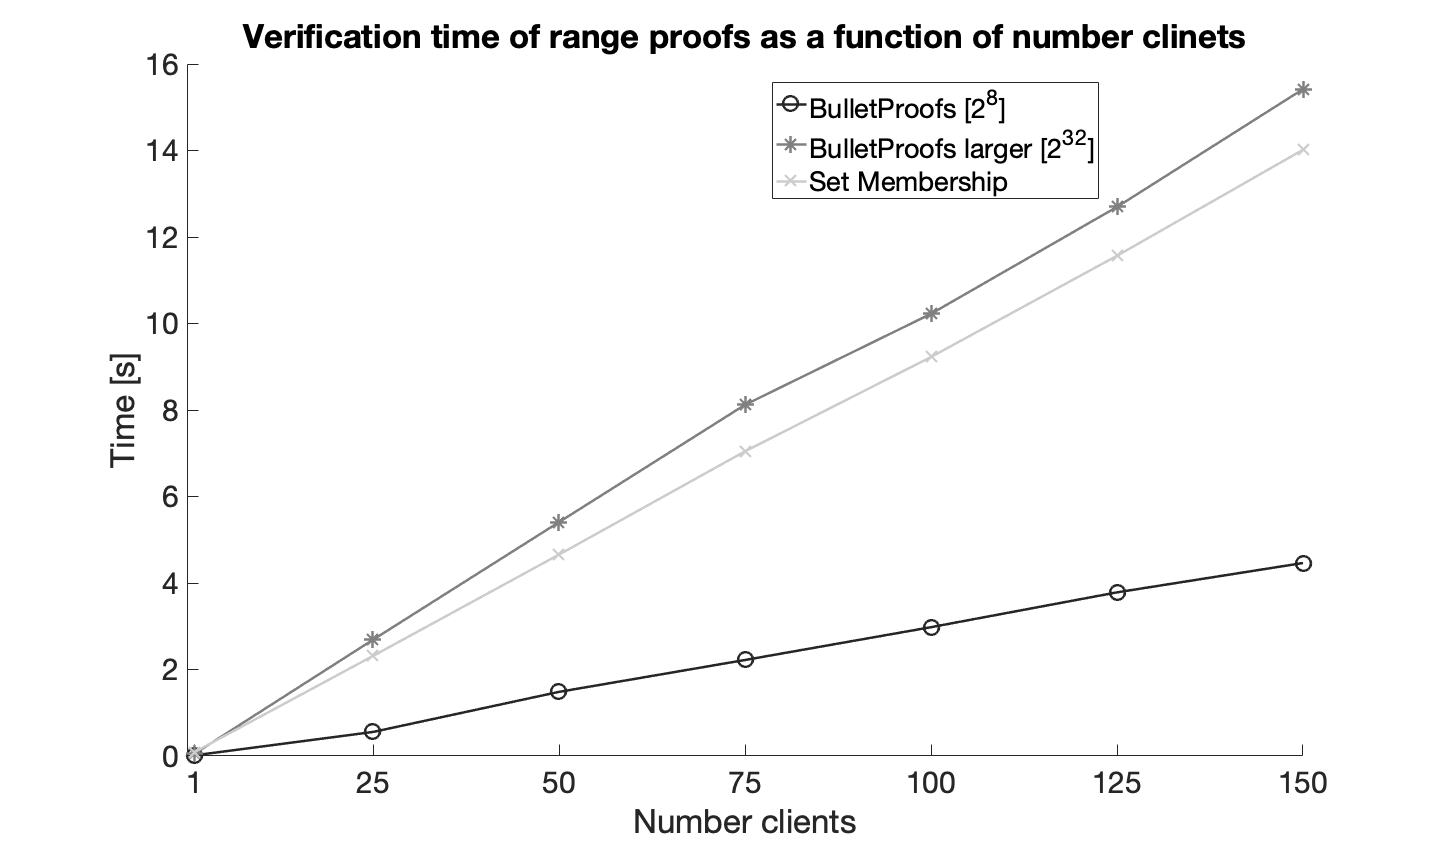
\includegraphics[width=\linewidth]{./figure/verification_nrClients.png}
%\end{figure}


% CONCLUSION
%You may consider to instead divide this chapter into discussion of the results and a summary. 
\chapter{Discussion and Conclusion}
\label{ch:Conslusion}
%In this chapter the a summary of the paper is given, where the most relevant results are pointed out and discussed. Followed by a section where possible extensions of the work and suggestions on related areas that would be interesting to investigate. Finally a short conclusion will be given. 
\section*{Discussion}
%naive aggregation
The simplest aggregation of set membership proofs is to construct the aggregated proof as the element-wise product of all individual proofs. Appendix \ref{appendix:naiveAgg} states how such an aggregation can be implemented. It also shows that it results in a construction that does not satisfy the completeness requirement of aggregated set membership proofs, implying that cleverer aggregation is required.

 Moreover, it is noted that if the challenges are equal for all proofs, then the completeness requirement is satisfied for the  first part of the validation. The challenges depend on randomness in the proofs, thereby it cannot be guaranteed that they are equal. In the aggregated signature-based set membership proof presented in chapter \ref{ch:AggSM} the challenges appear as a product, which resolves the problem of unequal challenges.

%partly aggregation
The complexity of the presented aggregated signature-based set membership proof depends on the number of provers, since  $a_i= e(V_i,y)^{c_i} e(V_i,g)^{-z_{x_i}}e(g,g)^{z_{\tau_i}}$ is checked separately for each proof $\Sigma_i$, $i\in\mathcal{S}$, in the verification. Therefore it can be interpreted as a partial aggregation  of the proofs. A complete aggregation of the signature-based set membership proofs fulfilling the completeness requirement has not been found nor proved impossible to construct. The reasoning of why a  complete aggregation of the signature-based set membership proofs does not fulfil the completeness requirement is given in appendix \ref{appendix:aggregate_a}. In the verification of the signature-based range proofs derived from the signature-based set membership proofs \cite{RANGE-SET}, the equality $a_i= e(V_i,y)^{c} e(V_i,g)^{-z_{x_i}}e(g,g)^{z_{\tau_i}}$ is checked separately for each $j\in\mathds{Z}_l$. This can be seen as an indicator that it is not possible to efficiently aggregate the entire signature-based set membership proofs. 

%Also aggregate RP follows
The presented construction of aggregated signature-based set membership proof can be translated to a construction of aggregated signature-based range proofs. The signature-based range proofs are very similar in construction to the signature-based set membership proofs and thereby the aggregation can easily be adjusted to aggregate the range proofs. Details on how to generalise the aggregation are not given, but it follows directly from inspection.
 
 %VAHSS clients can lie but not cheat
Using set membership proofs or range proofs to verify clients in a VAHSS construction prevents clients from cheating, but no requirement ensures that clients do not lie. Cheating means that a client shares a value not in the allowed set or range and lying means that the client shares a value in the allowed set or range, but not the truthful value.

%TODO Include : VAHSS not secure?
\section*{Conclusion}

% General def of agg and requirements
This paper has presented a definition of aggregated set membership proofs, including the completeness, soundness, and zero-knowledge requirements that it should fulfil.

% Aggregated signature based, partly wanted compleat
According to the definition of aggregated set membership proofs, signature-based set membership proofs have been partly aggregated. Since a part of the proofs is verified separately for each prover, the complexity for verification depends on the number of provers. However, the computational complexity required per prover is decreased, due to that, a part of the proofs is aggregated, such that it is checked once to validate all provers. 

% not trusted aggregation
It has been proved that an untrusted party must perform the aggregation according to the protocol, for the verification to validate true. The assumptions made to prove this are that: the provers do not collaborate  with each other or the aggregating party and that the aggregated proof $\Sigma_a$ is such that $D_a\neq C^c$. $C$ is the product of all provers Pedersen commitments and $c$ is the product of all challenges. 

% Proved C S ZK
The completeness, soundness and zero-knowledge requirements for aggregated set membership proofs are proved to hold for the presented construction of aggregated signature-based set membership proofs. This was proved under the assumptions that the aggregation was performed according to the algorithm \textbf{Aggregate}, proves does not collaborate and that the signature-based set membership, \cite{RANGE-SET}, satisfies the requirements in Definition \ref{def:ZKP}. 



%TODO implementation , Since a part of the proof is verified for each prover, 
The aggregated signature-based set membership proof has been implemented in Golang. Considering $100$ provers, each having constructed a signature-based set membership proof, the verification was found to be approximately $13\%$ faster for verifying an aggregated proof, computed according to algorithm \textbf{Agrgegate}, compared to verifying the proofs individually.  The prototype analysis also showed that splitting the aggregation between several parties decreased the runtime per aggregating party almost exponentially. The verification time, in tandem, does not increase exponentially.  

% Extended VAHSS
The second part of this paper focused on the verification of clients in VAHSS constructions and comparing different methods for verifying clients.  The VAHSS construction, presented in \cite{SumItUp} has been modified to additionally verify the clients. Clients are verified by publishing set membership proofs or range proofs. Then the verifier, in addition to validating the servers computations, validates all clients set membership proofs or range proofs. To reduce the computations required by the verifier aggregated set membership proofs are considered for verification of clients.

% Implemnetd extention
Implementations in Golang have been provided for the client and server VAHSS, considering Bulletproofs, aggregated and non-aggregated signature-based set membership proofs for verification of clients.



\section*{Future work}
In this section some question that has raised during the work is mentioned and discussed as possible future work.
\begin{itemize}
\item A complete aggregation of a set membership proofs. The presented aggregated signature-based set membership proof is partly aggregated and therefore the computational complexity of verification dependent on the number of provers.  Providing a full aggregation of the signature-based set membership proof or alternatively construct a complete aggregation of some other set membership proofs would be two interesting results.

\item Constructing a non-interactive aggregation of Bulletproofs. Bulletproofs are state of the art range proofs aggregating them using a non-interactive construction would be useful in many applications. To the knowledge of the author no such construction exists. 

\item Prio+, \cite{prioPlus}, constitutes the same purpose as client and server VAHSS. The computations required by the clients in Prio+ is smaller compare to client and server VAHSS, due to that they are not required to construct a ZKP. However, the servers must communicate to verify the clients.  An interesting topic would be to investigate if Prio+ can be modified such that the verification of clients can be obtained without communication between the servers and with a computational complexity independent of the number of clients. This would result in a construction highly efficient for both clients and servers. 
\end{itemize}



%Limit, only considerd range proof using pedersen commitment scheme.


%\textbf{FFS for intervals: }Need comunication between servers. We do not want 

%TODO very short

% REFERENCES / BIBLIOGRAPHY
\cleardoublepage
\addcontentsline{toc}{chapter}{Bibliography}
\bibliographystyle{abbrv}
\bibliography{ref.bib}

%\begin{thebibliography}{69}
\bibliography{bibliography.bib}
\bibitem{Reference} Frisk, D. (2016) A Chalmers University of Technology Master's thesis template for \LaTeX . Unpublished.

\bibitem{SumItUp} Tsaloli, G., and Mitrokotsa, A. (2020). Sum it up:  Verifiable additive homomorphic secret  sharing. In  J.  H.  Seo  (Ed.), Information  security  and  cryptology  –I CISC 2019 (pp. 115–132). Cham:  Springer International Publishing.

\bibitem{VHASS} Tsaloli, G., Banegas, G., and Mitrokotsa, A. (2020). Practical   and provably   secure   distributed aggregation: Verifiable   additive   homomorphic secret sharing. Cryptography, 4 (3). Retrieved from https://www.mdpi.com/2410-387X/4/3/25 doi:10.3390/cryptography4030025 

@article{How_share_A_secret,
author = {Shamir, Adi},
title = {How to Share a Secret},
year = {1979},
issue_date = {Nov. 1979},
publisher = {Association for Computing Machinery},
address = {New York, NY, USA},
volume = {22},
number = {11},
issn = {0001-0782},
url = {https://doi.org/10.1145/359168.359176},
doi = {10.1145/359168.359176},
journal = {Commun. ACM},
month = nov,
pages = {612–613},
numpages = {2}, 
keywords = {interpolation, key management, cryptography} }

\end{thebibliography}


% APPENDICES
\cleardoublepage
\appendix
\setcounter{page}{1}
\pagenumbering{Roman}			% Capitalized roman numbering starting from I (one)

%Bulletproof apendix instead refered to article
%\chapter{LHSS}
\label{appendix:VHASS-LSS}

\begin{algorithm}
\caption{\textbf{: Verifiable additive homomorphic secret sharing}}
\textbf{Goal:} Construct and share the sum $\sum_{i=1}^n x_i$, where $x_i$ is a secret value known by client $c_i$, where $i\in\mathcal{N}$ without any client needing to revealing their individual secret. The servers, used to sharing the secrets, computations are verified so they must be honest. 
\vspace{2pt}
\hline
\vspace{2pt}
\begin{itemize}
    \item\textbf{SetUp $1^\lambda, N$}
    Let $N$ be the product of two safe primes ($p,q$)  each of length $k'/2$. Choose at random two random safe primes $\hat{p},\hat{q}$ of length $k/2$, such that $\text{gcd}(N,\Phi(\hat{N}))=1$, where $\hat{N}=\hat{p}\hat{q}$. Then choose $g,g_1,g_2,h_1,...,h_n$ in $\mathds{Z}_{\hat{N}}$ at random. Choose an (efficiently computational) injective function $H:\{0,1\}^* \mapsto \{0,1\}^l$, with $l<k'/2$. Define the public verification key $vk= (N,H,\hat{N},g,g_1,g_2,h_1,...,h_n)$ and the private signing key to $sk=(\hat{p},\hat{q})$. 
  \item\textbf{ShareSecret $(1^\lambda,i,x_i)\xrightarrow[]{}(\{x_{ij}\}_{j\in\mathcal{M}})$}\\
Pick uniformly at random $\{a_i\}_{i\in\{1,..,t\}}\in\mathds{F}$ and a $t$-degree, put $x_{ij}=\lambda_{i,j}p_i(\theta_{ij})$.  Output $x_{i,j}$ for $j\in\mathcal{M}$. 

%, be a collision-resistant homomorphic hash function. Let $R_i\in\mathds{F}$ be the output of a PRF.$R_n = \phi(N)\lceil \frac{\sum_{i=1}^{n-1}R_i}{\phi(N)}\rceil- \sum_{i=1}^{n-1}R_i $. Compute $\tau_i = \mathcal{H}(x_i+R_i)$, 

\item\textbf{PartialEval $(j,\{x_{ij}\}_{i\in\mathcal{N}})\xrightarrow[]{}y_j$}\\
Compute and output $y_j = \sum_{i=1}^n x_{ij}$.

\item\textbf{PartialProof $(sk,vk,fid,x_i,i)\xrightarrow[]{}\sigma_j$}\\
Parse the verification key $vk$. Use the injective function $H$ to compute the prime $e=H(fid)$. Let $R_i\in\mathds{F}$ be the output of a PRF. $R_n, = \phi(N)\lceil \frac{\sum_{i=1}^{n-1}R_i}{\phi(N)}\rceil- \sum_{i=1}^{n-1}R_i $.  Choose at random $s_i\in_R\mathds{Z}_\hat{N}$ and use the secret key $sk$ to solve for $x$ in the equation $x^{eN}= g^{sj}\prod_{j=1}^n h_j^{f_j^{(i)}}g_1^{x_i+R_i} \: \text{mod}(\hat{N})$. Let the vector $f^{(i)}$ be the canonical bases $e_i$ of $\mathds{Z}^n$, this reduced the equation to $x^{eN}= g^{s_j} h_i g_1^{x_i+R_i} \: \text{mod}(\hat{N})$, set $\tilde{x}_i=x$ 
and output the partial proof $\sigma_i= (e,s_i,fid,\tilde{x}_i)$.

\item\textbf{ConstructRangeProof $x_i,i \mapsto proof_{RP}$}\\
Let $r_i\in\mathds{F}$ be the output of a PRF. $r_n, = \phi(N)\lceil \frac{\sum_{i=1}^{n-1}r_i}{\phi(N)}\rceil- \sum_{i=1}^{n-1}r_i $ and compute the Fujisaki-Okamoto commitment $\pi_i=g_1^{x_i}g_2^{r_i}$.
Use the commitment $\pi_i$ to construct a square-based range proof for the secret $x_i$ denoted $proof_{RP}$. Output $(\pi_i,proof_{RP_i})$.
 
\item\textbf{FinalEval $(\{y_j\}_{j\in\mathcal{M}})\xrightarrow[]{}y$}\\
Compute and output $y = \sum_{j=1}^m y_{j}$.

\item\textbf{FinalProof $(vk,\sigma_1,...,\sigma_n)\xrightarrow[]{}\sigma$}\\
Parse the partial proofs $\sigma_i$ to get $(e,s_i,fid,\tilde{x}_i,\pi_i)$.  
Let $\hat{f}= (\alpha_1,...,\alpha_n)\in\mathds{Z}^n$ and define $f' = ( \sum_{i=1}^n \alpha_if^(i)-f)/(eN)$, where $f=\sum_{i=1}^n\alpha f^{(i)} \: \text{mod}\:eN$. Set $s= \sum_{i=1}^n\alpha_is_i \: \text{mod}\:eN$, $s' = (\sum_{i=1}^n \alpha_i s_i -s)/eN \: \text{mod}\: eN$ and $\tilde{x} = \frac{\prod_{i=1}^n \tilde{x}_i^{\alpha_i}}{g^{s'}\prod_{j=1}^n h_j ^{f'}} \: \text{mod}\: \hat{N}$. Let $\alpha_i =1 \: \forall i\in\{1,...,n\}$, then compute  $\tilde{x} = \frac{\prod_{i=1}^n \tilde{x}_i}{g^{s'}\prod_{j=1}^n h_j ^{f'}} \: \text{mod}\: \hat{N}$.

Output the final proof $\sigma = (e,s,fid,\tilde{x})$.

\item\textbf{Verify $(vk,f,\sigma,y,\pi_i,...,\pi_n,proof_{RP_1},...,proof_{RP_n})\xrightarrow[]{}\{0,1\}$}\\
Compute $e=H(fid)$. Check that $y,s\in\mathds{Z}_\hat{N}$ and $\tilde{x}^{eN} = g^s\prod_{j=1}^n h_j^{f}g_1^y$. Further check that $g_1^y =\prod_{i=1}^n \pi_i$ and \textbf{VerifyRP}$(\pi_i,proof_{RP_i})\: \forall i\in\mathcal{N}$ 
\end{itemize}
\label{alg:VAHSS-LSS}
\end{algorithm}

\section*{Questions}
\begin{itemize}
\item Would it be possible to let $x$ be the solution to $x^{eN} = g^{s_j}h_ig_1^{x_i}g_2^{R_i} =  g^{s_j}h_i\pi_i $
\end{itemize}
\section*{Correctness, Securist and Verifiability}
\begin{itemize}
    \item \textbf{Correctness} Need to show $\text{Pr}[\textbf{Verify}(vk,f,\sigma,y\pi_1,...,\pi_n,proof_{RP_1},...,proof_{RP_n}) = 1] = 1$. For this it requires to show that all three following holds at the same time
    \begin{enumerate}
        \item $\tilde{x}^{eN} \overset{?}{=} g^s (\prod_{i=1}^n h_i^f )g_1^y$ \quad \quad (\textit{Holds given that} $y=\sum_{i=1}^n x_i$ ) 
        \item $g_1^y \overset{?}{=} \prod_{i=1}^n \pi_i$ \quad \quad (\textit{Holds given that $x_i=\sum_{j=1}^m x_{ij}$ and $\pi_i = g_1^{\hat{x}_i}g_2^{r_i}$ such that $x_i = \hat{x}_i$} ) 
        \item $\textbf{VerifyRP}(\pi_i,proof_{RP_i})\overset{?}{=}1 \: \forall i\in\mathcal{N}$ (\textit{Holds given that $x_i\in [a,b]\: \forall i\in\mathcal{N}$} ) 
    \end{enumerate}  
    The first statement is proved to hold by original VAHSS-LHS. For the seconds statment it holds that;
    \begin{align*}
        LHS = g_1^y = g_1^{\sum_{j=1}^m y_{j}} \overset{*}{=} g_1^{\sum_{j=1}^m \sum_{i=1}^n x_{ij}}
 = g_1^{\sum_{i=1}^n x_{i}} \text{ *Due to first statement.} \\
 RHS = \prod_{i=1}^n \pi_i = \prod_{i=1}^n g_1^{x_i}g_2^{r_i} = g_1^{\sum_{i=1}^n x_i} g_2 ^{\sum_{i=1}^n r_i} =  g_1^{\sum_{i=1}^n x_i}.  \implies LHS = RHS
 \end{align*} 
 
 The last follows from the verification of a correctly constructed range proof.
 
 \item\textbf{Security} 
 
 \item \textbf{Verifiability}
    \begin{itemize}
        \item If $x_i=\sum_{j=1}^m x_{ij}$,  $\pi_i = g_1^{\hat{x}_i}g_2^{r_i}$  and  $x_i \neq \hat{x}_i$, then,
        \begin{align*}
            g_1^y = \prod_{i=1}^n \pi_i \implies
            g^{\sum_{i=1}^n x_{i}} =  g^{\sum_{i=1}^n \hat{x}_{i}} \implies \\
            \sum_{i=1}^n x_{i} = \sum_{i=1}^n \hat{x}_{i} \text{ (Contraction)}
        \end{align*}
    \end{itemize}
\end{itemize}

% multiple aggregators
\chapter{Multiple Aggregating Parties}
\label{app:manyAggregatingParties}


\begin{comment}
Let $x=\sum_{j=0}^{l-1} x_j u^j$, where $x_j$ is an integer and $x_j\in[0,u)$, $u,l$ are integers and $j\in[0,l-1] (=\mathds{Z}_l)$. Then it holds that $x\in[0,u^l)$.
\begin{align*}
x =& \sum_{j=0}^{l-1} x_j u^j \leq \sum_{j=0}^{l-1}  (u-1)u^j = \sum_{j=0}^{l-1} u^{j+1} - \sum_{j=0}^{l-1} u^j = (u-1) \sum_{j=0}^{l-1} u^j =\\
 &(u-1) \frac{u^l-1}{u-1} = u^l-1< u^l 
\end{align*}
Hence the  statement is proved and it is trivial to see that if $j\in[0,l]$ the value of $x$ could exceed $u^l$.
\end{comment}
\begin{comment}
\begin{algorithm}
\caption{\textbf{: Client and Server Verifiable additive homomorphic secret sharing}}

\textbf{Goal:} Given  Pedersen commitments $C_i=g^{x_i} h^{R_i}$, for $i\in\mathcal{S}$. The construction  proves that all secrets $x_i$ belongs to the set $\Phi$, without revealing anything else about the secrets.
\vspace{2pt}
\hline
\vspace{2pt}
\begin{itemize}
 \item\textbf{ShareSecret $(1^\lambda,i,x_i) \mapsto \{x_{ij}\}_{j\in\mathcal{M}}$} \\
Pick uniformly at random $\{a_i\}_{i\in\{1,..,t\}}\in_R\mathds{F}$ to be the coefficients to a $t$-degree polynomial $p_i$ on the form $p_i(X) = x_i + a_1X+...+a_tX^t$. Define  the shares as $x_{ij}=\lambda_{i,j}p_i(\theta_{ij})$ for $j\in\mathcal{M}$, the parameters $\theta_{ij}$ and Lagrange coefficients $\lambda_{ij}$ is chosen such that equation \ref{eq:pi(0)} is satisfied.
Output $\{x_{ij}\}_{j\in\mathcal{M}}$.

\item\textbf{GenereteCommitment$(1^\lambda,i,x_i) \mapsto \pi_i$ }\\
Let $\mathds{E} : x,y \to g^xh^y$ be a Pedersen commitment . Let $R_i\in\mathds{F}$ be the output of a PRF such that $R_n\in \mathds{F}$  satisfies $R_n = \phi(N)\lceil \frac{\sum_{i=1}^{n-1}R_i}{\phi(N)}\rceil- \sum_{i=1}^{n-1}R_i $. Compute and output $\pi_i = \mathds{E}(x_i,R_i)$.

\item\textbf{RangeProof $(x_i,\pi_i) \mapsto RP_i$}\\
Construct a range proof, denoted $RP_i$, for the commitment $\pi_i$ to the secret $x_i$, on the set $\Phi$ using the agorithm \textbf{Prove} in Construction \ref{alg:ZKSM-Agg}. All required  parameters and setup is assumed to be pre-shared and known by all parties.

\item\textbf{PartialEval $(j,\{x_{ij}\}_{i\in\mathcal{N}})\xrightarrow[]{}y_j$}\\
Compute and output $y_j = \sum_{i=1}^n x_{ij}$.

\item\textbf{PartialProof $(j,\{x_{ij}\}_{i\in\mathcal{N}})\xrightarrow[]{}\sigma_j$}\\
Compute and output $\sigma_j = \prod_{i=1}^n g^{x_{ij}} =  g^{\sum_{i=1}^n x_{ij}}= g^{y_j}=H(y_j)$.

\item \text{\textbf{PartialAggregate} $(g,h, \mathcal{S}\{ \textit{proof}_{SM,i}\}_{i\in\mathcal{S}} \xrightarrow[]{} \texit{proof}_{SM,a}$} \\
Given a subset of range proofs  $\{ \textit{proof}_{SM,i}\}_{i\in\mathcal{S}}$ where $\mathcal{S}\subseteq \{1,...,n\}$. Aggregate the values $\{D_i \}_{i\in\mathcal{S} } \{ z_{x_i}\}_{i\in\mathcal{S} } \{ z_{r_i}\}_{i\in\mathcal{S} } \mapsto D_a,z_{x_a},z_{R_a}$ according to equation \eqref{eq:aggDn}. Then construct and publish the aggregated range proof $\texit{proof}_{SM,a} = (\{V_i\}_{i\in\mathcal{S} },\{a_i\}_{i\in\mathcal{S} },D_a,\{z_{x_i}\}_{i\in\mathcal{S} }, z_{x_a}, \{z_{\tau_i}\}_{i\in\mathcal{S} },z_{R_a})$.


\item\textbf{FinalEval $(\{y_j\}_{j\in\mathcal{M}})\xrightarrow[]{}y$}\\
Compute and output $y = \sum_{j=1}^m y_{j}$.

\item\textbf{FinalProof $(\{\sigma_j\}_{j\in\mathcal{M}})\xrightarrow[]{}\sigma$}\\
Compute and output $\sigma = \prod_{j=1}^m \sigma_j = \prod_{j=1}^m g^{y_{j}} =  g^{\sum_{j=1}^m y_{j}}= g^{y}=H(y)$.

\item\textbf{Verify $(\{\pi_i\}_{i\in\mathcal{N}},x,y,\{RP_{a_i}\}_{i\in\mathcal{M}})\xrightarrow[]{}\{0,1\}$}\\
Compute and output $\sigma= \prod_{i=1}^n \pi_i \wedge \prod_{i=1}^n \pi_i = H(y)\wedge \{\textbf{VerifyAggregatedProof}(RP_{a_i})\}_{i\in\mathcal{M}}$. Where $\textbf{VerifyAggregatedProof}$ is the verification algorithm in Construction \ref{alg:VAHSS-HSS-RP-Agg}.
\end{itemize}
\label{alg:VAHSS-HSS-RP-Agg}
\end{algorithm}

\end{comment}

\begin{algorithm}[]
\caption{\textbf{: Aggregation of non interactive set membership proof}}
%This protocol is a modification of Construction \ref{alg:ZKSM}, such that when multiple parties wish to prove that their secret is in an allowed set, $\Phi$, to the same verifier, their proofs can be partly aggregated into one common proof to reduce the verification time. 
\textbf{Goal:}  Given  the Pedersen commitments $C_i=g^{x_i} h^{R_i}$, for $i\in\mathcal{S}$. The construction  proves that all secrets $x_i$ belongs to the set $\Phi$, without revealing anything else about the secrets.
\vspace{2pt}\hrule\vspace{2pt}
\begin{itemize}
 \item\textbf{SetUp $(1^\lambda,\Phi)\xrightarrow[]{}(sk,pp)$}\\
 Let g be a generator of the group $\mathds{G}$ and $h$ an element in the group such that $log_g(h)$ is unknown.  
Pick uniformly at random $\chi\in_R\mathds{F}$ and put $sk=\chi$. Define $y=g^\chi$ and $A_i=g^{\frac{1}{\chi+i}} \:\forall i\in\Phi$, output $pp=(g,h,y,\{A_i\}_{i\in\Phi})$.

\item\text{\textbf{Prove} $(pp,i,C_i,x_i,\Phi)\xrightarrow[]{} \Sigma_i$}\\
Pick uniformly at random $\tau_i\in_R\mathds{F}$, choose from the set $\{A_i\}$ the element $A_{x_i}$ and calculate $V_i=A_{x_i}^{\tau_i}$. Pick uniformly at random three values $s_i,t_i,m_i\in_R\mathds{F}$. Put $a_i=e(V_i,g)^{-s_i}e(g,g)^{t_i}$,  $D=g^{s_i}h^{m_i}$,$c=\text{Hash}(C_i,V_i,a_i,D_i)$ and compute $z_{x_i} = s_i-x_i c_i$, $z_{R_i} = m_i-R_ic_i$ and $z_{\tau_i}= t_i-\tau_i c_i$ . Finally construct and publish the proof $\Sigma_i = (V_i,a_i,D_i,z_{x_i},z_{\tau_i},z_{R_i})$.

\item \text{\textbf{Aggregate} $( pp,k,\{ \Sigma_i\}_{i\in\mathcal{S}_k} ) \xrightarrow[]{} \Sigma_{a_k}$} \\
Given a set of  proofs  $\{\Sigma_i\}_{i\in\mathcal{S}_k}$. Aggregate the values $( \{D_i \}_{i\in\mathcal{S}_k }, \{ z_{x_i}\}_{i\in\mathcal{S}_k }, \{ z_{r_i}\}_{i\in\mathcal{S}_k  }) \mapsto D_{a_k},z_{x_{a_k}},z_{R_{a_k}}$ according to equation \eqref{eq:aggDn}. Construct and publish the aggregated proof $\Sigma_{a_k} = (\{V_i\}_{i\in\mathcal{S}_k },\{a_i\}_{i\in\mathcal{S}_k },D_{a_k},\{z_{x_i}\}_{i\in\mathcal{S}_k }, z_{x_{a_k}}, \{z_{\tau_i}\}_{i\in\mathcal{S}_k },z_{R_{a_k}})$.

\item \text{ \textbf{CalculateChallenges} $(\{C_i\}_{i\in\mathcal{S}}, \{\Sigma_i\}_{i\in\mathcal{S}} ) \xrightarrow[]{} \{c_i\}_{i\in\mathcal{S}}$ }\\
For all $i\in\mathcal{S}$ parse the proof $\Sigma_i$, then compute the challenge $c_i = Hash(C_i,V_i,a_i,D_i)$. Finally output the set of all challenges $\{c_i\}_{i\in\mathcal{S}}$. 

\item\text{\textbf{Verify} $(pp,\{\Sigma_{a_k}\}_{k\in\mathcal{K}},\{C_i\}_{i\in\mathcal{S}},\{c_i\}_{i\in\mathcal{S}}) \xrightarrow[]{} \{0,1\}$} \\
For all $k\in\mathcal{K}$ compute the product of the challenges $c_k=\prod_{i\in\mathcal{S}_k} c_i$. Check if $D_{a_k}\overset{?}{=} \big( \prod_{i\in\mathcal{S}_k} C_i\big)^{c_k}h^{z_{R{a_k}}}g^{z_{x{a_k}}}$ 
Then for check if $ a_i \overset{?}{=} e(V_i,y)^c_i e(V_i,g)^{-z_{x_i}}e(g,g)^{z_{\tau_i}}$ for all $i\in\mathcal{S}$. If the equalities holds return $1$ otherwise return $0$.
\end{itemize}
\label{alg:ZKSM-Agg-Many}
\end{algorithm} 

% naive aggrgeation element-wise
\chapter{Naive Aggregation }
\label{appendix:naiveAgg}
Consider two set membership proofs $\Sigma_1$ and $\Sigma_2$, computed according to the algorithm \textbf{Prove} in Construction \ref{alg:ZKSM-Agg}. The proofs are on the form $\Sigma_i = (V_i,a_i,D_i,z_{x_i},z_{\tau_i},z_{R_i})$ for $i=1,2$.  Denote the challenges used to construct the proofs $c_i$ for $i=1,2$ and the related Pedersen commitments are denoted $C_i$  for $i=1,2$.

The naive construction of the algorithm \textbf{Aggregate} is to
define the aggregated proof, $\Sigma_a$, as the  element-wise product or addition of the two proof $\Sigma_1$ and $\Sigma_2$. This yields that $\Sigma_a = (V_a,a_a,D_a,z_{x_a},z_{\tau_a },z_{R_a})$, where $V_a, a_a, D_a,z_{x_a},z_{\tau_a },z_{R_a}$ are computed as,
\begin{equation}
\begin{aligned}
\label{eq:naiveAgg}
V_a =& V_1V_2 = g^{\frac{\tau_1}{\chi + x_1}}g^{\frac{\tau_2}{\chi + x_2}}\\
a_a =& a_1a_2 = \big( e(g,g)^{\frac{-s_1\tau_i}{\chi+x_1}}e(g,g)^{t_1}\big) \big( e(g,g)^{\frac{-s_2\tau_2}{\chi+x_2}}e(g,g)^{t_2}\big) \\
D_a =& D_1D_2 = ( g^{s_1}h^{m_1} ) (g^{s_2} h^{m_2}) = g^{s_1+s_2}h^{m_1+m_2}\\
z_{x_a} =& z_{x_1} + z_{x_2} = (s_1-c_1x_1)+(s_2-c_2x_2)\\
z_{R_a} =& z_{R_1} + z_{R_2} = (m_1-c_1R_1)+(m_2-c_2R_2)\\
z_{\tau_a} =& z_{x_1} + z_{x_2} = (t_1-c_1\tau_1)+(t_2-c_2\tau_2)\\ 
\end{aligned} 
\end{equation}

$C=C_1C_2 = g^{x_1+x_2}h^{R_1+R_2}$ is the product of the two Pedersen commitments and $c=c_1c_2$ denotes the product of the challenges .

Investigated if the aggregated proof $\Sigma_a$ satisfies the equations: $D_a = C^ch^{z_{R_a}}g^{z_{x_a}}$ and  $a_a \overset{?}{=} e(V_a,y)^ce(V_a,g)^{-z_{x_a}}e(g,g)^{z_{\tau_a}}$.

Considering the first equality it follows that.
\begin{align*}
&D_a = g^{s_1+s_2}h^{m_1+m_2} \\
&C^ch^{z_{R_a}}g^{z_{x_a}} =\: ... \:= g^{s_1+s_2} h^{m_1+m_2} g^{c(x_1+x_2) - c_1x_1 -c_2x_2}h^{c(R_1+R_2)-R_1c_1-R_2c_2} \\
\implies & D_a \neq C^ch^{z_{R_a}}g^{z_{x_a}} 
\end{align*}

Thereby the completeness property is not satisfied for the aggregated proof $\Sigma_a$. The equality does not hold due to the $ c(x_1+x_2)  \neq x_1c_1 + x_2c_2$. Note that if $c_1=c_2=c$ then the above is an equality.

%aggregation of a
\chapter{Complete Aggregation }
\label{appendix:aggregate_a}
To fully aggregate the signature-based set membership proofs the verification would need to be independent of the number of provers. 

Consider two set membership proofs $\Sigma_1$ and $\Sigma_2$ computed according to the algorithm \textbf{Prove} in Construction \ref{alg:ZKSM-Agg}. The proof $\Sigma_i = (V_i,a_i,D_i,z_{x_i},z_{\tau_i},z_{R_i})$ for $i=1,2$. Denote the Pedersen commitments by $C_i$ and the challenges $c_i$, for $i=1,2$.
It will be assumed, although unrealistic for non interactive constructions of set membership proof, that $c=c_1=c_2$.
%and $V_i =  g^{\frac{\tau_i}{q+x_i}}, 
%a_i = e(V_i,g)^{s_i}e(g,g)^{t_i}, \:
%D_i =  g^{s_i}h^{m_i}, \:
%z_{x_i} =  s_i- c x_i, \:
%z_{\tau_i} = t_i- c \tau_i$ and 
%$z_{R_i} =  m_i+ c R_i$, 
%where $s_i,t_i,m_i \in_R \mathds{F}$ ,  $g,h$ are group elements of the group $\mathds{G}$, $q$ is a secret key not known by any party, $y=g^q$ is the public key known to any party. The, here assumed same for both parties, challenge is denoted$c$ and is publicly known, and finally $x_i, R_i$ denoted the secret and randomness of prover $i=1,2$ 

The aim is to investigate if the two proofs can be aggregated into the aggregated proof, $\Sigma_a=(V_a,a_a,D_a,z_{x_a}, z_{\tau_a}, z_{R_a})$ , such that $a_a \overset{?}{=} e(V_a,y)^c e(V_a,g)^{-z_{x_a}}e(g,g)^{z_{\tau_a}}$ holds and that equality implies that $x_i\in\Phi$ for $i=1,2$. 

The aggregation is performed according equation \eqref{eq:naiveAgg}, using $c$ as the challenge. This given that,
\begin{align*}
& a_a = e(g,g) ^{\frac{\tau_1 s_1}{q+x_1} \frac{\tau_2 s_2}{q+x_2} +t_1+t_2} 
\\
& e(V_a,y)^ce(V_a,g)^{-z_{x_a}}e(g,g)^{z_{\tau_a}}  = \: ... \:= 
  e(g,g)^{ \frac{s_1 \tau_1}{q+x_1}+t_1} e(g,g)^{ \frac{s_2 \tau_2}{q+x_2}+t_2}   e(V_1,g)^{- z_{x_2} }   e(V_2,g)^{ - z_{x_1} }
   \\
 & \implies a_a \neq e(V_a,y)^ce(V_a,g)^{-z_{x_a}}e(g,g)^{z_{\tau_a}} 
\end{align*}
%e(V_1V_2,y)^ce(V_1V_2,g)^{-z_{x_1}- z_{x_2}}e(g,g)^{z_\tau_1+z_\tau_2} \\
%=& e(g,g)^{cq \big (  \frac{\tau_1}{q+x_1} + \frac{\tau_2}{q+x_2}\big) } e(g,g)^{ \big(-(s_1- c x_1) - (s_2 - c x_2)  \big) \big (  \frac{\tau_1}{q+x_1} + \frac{\tau_2}{q+x_2}\big) } e(g,g)^{ (t_1- c \tau_1) +(t_2- c \tau_2)} \\
 %= & e(g,g)^{ \frac{\tau_1}{q+x_1} \Big(  cq- (s_1-cx_1) -(s_2-cx_2) -c(q+x_1) \Big)+ t_1 }  e(g,g)^{ \frac{\tau_2}{q+x_2} \Big(  cq - (s_1-cx_1)- (s_2-cx_2) + c)(q+x_2) \Big)+ t_2 } \\
 %= &  e(g,g)^{ \frac{s_1 \tau_1}{q+x_1}+t_1}  e(g,g)^{ \frac{\tau_1}{q+x_1} \Big(  cq + cx_1 - c(q+x_1) - (s_2-cx_2) \Big) }  \\
% &e(g,g)^{ \frac{s_2 \tau_2}{q+x_2} + t_2  }  e(g,g)^{ \frac{\tau_2}{q+x_2} %\Big(  cq + cx_2 - c(q+x_2) - (s_1-cx_1) \Big) } \\
% = &  e(g,g)^{ \frac{s_1 \tau_1}{q+x_1}+t_1} e(g,g)^{ \frac{s_2 \tau_2}{q+x_2}+t_2}   e(g,g)^{ \frac{\tau_1}{q+x_1} \Big(  - (s_2-cx_2) \Big) }   e(g,g)^{ \frac{\tau_2}{q+x_2} \Big( - (s_2-cx_2) \Big) } \\
% = & %

Even under the assumption that $c= c_1=c_2$, the terms $e(V_1,g)^{- z_{x_2} }   e(V_2,g)^{ - z_{x_1} }$ are not cancelled. Thereby, although the aggregation is performed such that the challenges only appears as a product the completeness property does not hold.  






\end{document}
